\documentclass[openany,oneside,10pt]{memoir}

\usepackage{../forallxyyc}

\IfFileExists{../forallxyyc-local.sty}{\usepackage{../forallxyyc-local}}{}

\hypersetup{pdfinfo={Title={forall x: Calgary Remix. Solutions to Selected Exercises}, Author={P.D. Magnus, Tim Button, J. Rob Loftis, Robert Trueman, Aaron Thomas-Bolduc, Richard Zach}, Subject={An open access introductory textbook in formal logic}, Keywords={truth-functional logic, propositional logic, predicate logic, first-order logic, natural deduction, fitch, modal logic}}, 
  bookmarks={true}, 
  bookmarksopen = {true},
        colorlinks={true}, 
        allcolors={dkleadbeater},
        pdfdisplaydoctitle={true}}

\usepackage[absolute,overlay]{textpos}

% set stock & paper size with narrow margins

\setstocksize{8in}{5in}

\settrimmedsize{\stockheight}{\stockwidth}{*}
\settrims{0pt}{0pt}

% let's calculate the line length for 65 characters in \normalfont

\setlxvchars

% set the size of the type block to golden ratio calculated width

\settypeblocksize{*}{1.05\lxvchars}{1.62}

% set spine and and edge margin

\setlrmargins{*}{*}{1}
\setulmargins{.6in}{*}{*}
\setheaderspaces{*}{*}{1}

\checkandfixthelayout

\definecolor{lyallpink}{RGB}{222,31,149}
\colorlet{leadbeater}{lyallpink}
\colorlet{dkleadbeater}{lyallpink!80!black}
\colorlet{ltleadbeater}{lyallpink!50}
\colorlet{vltleadbeater}{lyallpink!3}

\begin{document}
\midsloppy

\pagestyle{leadbeater}

\frontmatter
%!TEX root = forallxyyc.tex
\thispagestyle{empty}  \pagecolor{darkred}\color{white}

\noindent {\fontsize{46pt}{0pt}\selectfont forall $x$}

\

\noindent{\Huge{Calgary Remix}}

\bigskip\bigskip
\noindent{\Huge \emph{Solutions to Selected Exercises}}

\vspace*{50pt}
\noindent\fontsize{16pt}{18pt}\selectfont \textit{By } \textbf{P.~D. Magnus}\\
\textbf{Tim Button}\\
\textit{with additions by}\\
\textbf{J.~Robert Loftis}\\
\textit{remixed and revised by}\\
\textbf{Aaron Thomas-Bolduc}\\ \textbf{Richard Zach}

\vfill

\noindent\normalsize

\includegraphics[width=1cm]{../assets/cc.pdf}

\includegraphics[width=1cm]{../assets/by}

\includegraphics[width=1cm]{../assets/remix}
\hfill \vbox to 1cm{\vfill\hbox{\LARGE \forallxversion}\vfill}

\newpage\nopagecolor\color{black}
\noindent This booklet is based on the solutions booklet \href{http://people.ds.cam.ac.uk/tecb2/forallx.shtml}{\forallx:\emph{ Cambridge}}, by\\[2ex]
\href{http://people.ds.cam.ac.uk/tecb2/index.shtml}{Tim Button}\\
\emph{University of Cambridge}\\[2ex]
used under a \href{https://creativecommons.org/licenses/by/4.0/}{CC BY 4.0} license, which is based in turn on \href{https://www.fecundity.com/logic/}{\forallx}, by\\[2ex]
\href{https://www.fecundity.com/job/}{P.D.\ Magnus}\\
\emph{University at Albany, State University of New York}\\[2ex]
used under a \href{https://creativecommons.org/licenses/by/4.0/}{CC BY 4.0} license,
\\
which was remixed \& expanded by\\[2ex] {Aaron Thomas-Bolduc \& Richard Zach}\\
\emph{University of Calgary}
\\
\\
It includes additional material from \forallx{} by P.D. Magnus, used under
a \href{https://creativecommons.org/licenses/by/4.0/}{CC BY 4.0}
license, and from \href{https://github.com/rob-helpy-chalk/openintroduction}{\forallx: \emph{Lorain County Remix}}, by \href{https://sites.google.com/site/cathalwoods/}{Cathal
Woods} and J. Robert Loftis, used with permission.

\bigskip

\noindent This work is licensed under a \href{https://creativecommons.org/licenses/by/4.0/}{Creative Commons Attribution 4.0} license. 
You are free to copy and redistribute the material in any medium or format, and  remix, transform, and build upon the material for any purpose, even commercially, under the following terms:
\begin{itemize}
\item You must give appropriate credit, provide a link to the license, and indicate if changes were made. You may do so in any reasonable manner, but not in any way that suggests the licensor endorses you or your use.
\item You may not apply legal terms or technological measures that legally restrict others from doing anything the license permits.
\end{itemize}
The \LaTeX{} source for this book is available on \href{https://github.com/rzach/forallx-yyc/}{GitHub}. This version
is revision \gitAbbrevHash{} (\gitAuthorDate).


\vfill
\noindent The preparation of this textbook was made possible by a grant from the \href{http://www.ucalgary.ca/taylorinstitute/}{Taylor Institute for Teaching and Learning}.

\bigskip
\noindent
\href{http://www.ucalgary.ca/taylorinstitute/}{
\includegraphics[width=8cm]{../assets/ti-color}}


\currentpdfbookmark{Table of Contents}{name}
\tableofcontents*

\mainmatter
%!TEX root = forallxsol.tex
%\part{Key notions}
%\label{ch.intro}
%\addtocontents{toc}{\protect\mbox{}\protect\hrulefill\par}

\chapter{Arguments}
Highlight the phrase which expresses the conclusion of each of these arguments:
\begin{earg}
	\item It is sunny. So \myanswer{I should take my sunglasses}.
	\item \myanswer{It must have been sunny}. I did wear my sunglasses, after all.
	\item No one but you has had their hands in the cookie-jar. And the scene of the crime is littered with cookie-crumbs. \myanswer{You're the culprit}!
	\item Miss Scarlett and Professor Plum were in the study at the time of the murder. And Reverend Green had the candlestick in the ballroom, and we know that there is no blood on his hands. Hence \myanswer{Colonel Mustard did it in the kitchen with the lead-piping}. Recall, after all, that the gun had not been fired.
\end{earg}

\chapter{Valid arguments}
\problempart
Which of the following arguments is valid? Which is invalid?

\begin{earg}
\item Socrates is a man.
\item All men are carrots.
\item[$\therefore$]  Socrates is a carrot. \hfill \myanswer{Valid}
\end{earg}

\begin{earg}
\item Abe Lincoln was either born in Illinois or he was once president.
\item Abe Lincoln was never president.
\item[$\therefore$] Abe Lincoln was born in Illinois. \hfill \myanswer{Valid}
\end{earg}

\begin{earg}
\item If I pull the trigger, Abe Lincoln will die.
\item I do not pull the trigger.
\item[$\therefore$] Abe Lincoln will not die. \hfill \myanswer{Invalid \\ Abe Lincoln might die for some other reason: someone else might pull the trigger; he might die of old age.}
\end{earg}

\begin{earg}
\item Abe Lincoln was either from France or from Luxemborg.
\item Abe Lincoln was not from Luxemborg.
\item[$\therefore$] Abe Lincoln was from France. \hfill \myanswer{Valid}
\end{earg}

\begin{earg}
\item If the world were to end today, then I would not need to get up tomorrow morning.
\item I will need to get up tomorrow morning.
\item[$\therefore$] The world will not end today. \hfill \myanswer{Valid}
\end{earg}

\begin{earg}
\item Joe is now 19 years old.
\item Joe is now 87 years old.
\item[$\therefore$] Bob is now 20 years old. \hfill \myanswer{Valid}
\\\myanswer{An argument is valid if and only if it is impossible for all the premises to be true and the conclusion false. It is impossible for all the premises to be true; so it is certainly impossible that the premises are all true and the conclusion is false.}
\end{earg}

\problempart
\label{pr.EnglishCombinations}
Could there be:
	\begin{earg}
		\item A valid argument that has one false premise and one true premise? \hfill \myanswer{Yes. \\Example: the first argument, above.}
		\item A valid argument that has only false premises? \hfill \myanswer{Yes.\\Example: Socrates is a frog, all frogs are excellent pianists, therefore Socrates is an excellent pianist.}
		\item A valid argument with only false premises and a false conclusion? \hfill \myanswer{Yes. \\The same example will suffice.}
		\item A sound argument with a false conclusion? \hfill\myanswer{No.\\ By definition, a sound argument has true premises. And a valid argument is one where it is impossible for the premises to be true and the conclusion false. So the conclusion of a sound argument is certainly true.}
		\item An invalid argument that can be made valid by the addition of a new premise? \hfill\myanswer{Yes.\\ Plenty of examples, but let me offer a more general observation. We can \emph{always} make an invalid argument valid, by adding a contradiction into the premises. For an argument is valid if and only if it is impossible for all the premises to be true and the conclusion false. If the premises are contradictory, then it is impossible for them all to be true (and the conclusion false).}
		\item A valid argument that can be made invalid by the addition of a new premise? \hfill \myanswer{No.\\ An argument is valid if and only if it is impossible for all the premises to be true and the conclusion false. Adding another premise will only make it harder for the premises all to be true together.}
	\end{earg}
In each case: if so, give an example; if not, explain why not.

\chapter{Other logical notions}
\setcounter{ProbPart}{0}
\problempart
\label{pr.EnglishTautology}
For each of the following: Is it necessarily true, necessarily false, or contingent?
\begin{earg}
\item Caesar crossed the Rubicon.
\hfill \myanswer{Contingent}
\item Someone once crossed the Rubicon.
\hfill \myanswer{Contingent}
\item No one has ever crossed the Rubicon.
\hfill \myanswer{Contingent}
\item If Caesar crossed the Rubicon, then someone has.
\hfill \myanswer{Necessarily true}
\item Even though Caesar crossed the Rubicon, no one has ever crossed the Rubicon.
\hfill \myanswer{Necessarily false}
\item If anyone has ever crossed the Rubicon, it was Caesar.
\hfill \myanswer{Contingent}
\end{earg}

\problempart
For each of the following: Is it a necessary truth, a necessary falsehood, or contingent?
\begin{earg}
\item Elephants dissolve in water.
\item Wood is a light, durable substance useful for building things.
\item If wood were a good building material, it would be useful for building things.
\item I live in a three story building that is two stories tall.
\item If gerbils were mammals they would nurse their young.
\end{earg}

\problempart Which of the following pairs of sentences are necessarily  equivalent? 

\begin{earg}
\item Elephants dissolve in water.	\\
	If you put an elephant in water, it will disintegrate.
\item All mammals dissolve in water.\\		
	If you put an elephant in water, it will disintegrate. 
\item George Bush was the 43rd president. \\
	 Barack Obama is the 44th president. 
\item Barack Obama is the 44th president. \\
	  Barack Obama was president immediately after the 43rd president. 
\item Elephants dissolve in water. 	\\	
	All mammals dissolve in water. 
\end{earg}

\problempart Which of the following pairs of sentences are necessarily equivalent? 

\begin{earg}
\item  Thelonious Monk played piano.	\\
	John Coltrane played tenor sax. 
\item  Thelonious Monk played gigs with John Coltrane.	\\
	John Coltrane played gigs with Thelonious Monk.
\item  All professional piano players have big hands.	\\
	Piano player Bud Powell had big hands.
\item  Bud Powell suffered from severe mental illness.	 \\
	All piano players suffer from severe mental illness.
\item John Coltrane was deeply religious.	 \\
John Coltrane viewed music as an expression of spirituality. 
\end{earg}

\noindent \problempart Consider the following sentences: 
\begin{enumerate}%[label=(\alph*)]
\item[G1] \label{itm:at_least_four}There are at least four giraffes at the wild animal park.
\item[G2] \label{itm:exactly_seven} There are exactly seven gorillas at the wild animal park.
\item[G3] \label{itm:not_more_than_two} There are not more than two Martians at the wild animal park.
\item[G4] \label{itm:martians} Every giraffe at the wild animal park is a Martian.
\end{enumerate}

Now consider each of the following collections of sentences. Which are jointly possible? Which are jointly impossible?
\begin{earg}
\item G2, G3, and G4
\hfill \myanswer{Jointly possible}
\item G1, G3, and G4
\hfill \myanswer{Jointly impossible}
\item G1, G2, and G4
\hfill \myanswer{Jointly possible}
\item G1, G2, and G3
\hfill \myanswer{Jointly possible}
\end{earg}

\problempart Consider the following sentences.
\begin{enumerate}%[label=(\alph*)]
\item[M1] \label{itm:allmortal} All people are mortal.
\item[M2] \label{itm:socperson} Socrates is a person.
\item[M3] \label{itm:socnotdie} Socrates will never die.
\item[M4] \label{itm:socmortal} Socrates is mortal.
\end{enumerate}
Which combinations of sentences are jointly possible? Mark each ``possible'' or ``impossible.''
\begin{earg}
\item Sentences M1, M2, and M3
\item Sentences M2, M3, and M4
\item Sentences M2 and M3
\item Sentences M1 and M4
\item Sentences M1, M2, M3, and M4
\end{earg}

\problempart
\label{pr.EnglishCombinations2}
Which of the following is possible? If it is possible, give an example. If it is not possible, explain why.
\begin{earg}
\item A valid argument that has one false premise and one true premise

\item A valid argument that has a false conclusion

\item A valid argument, the conclusion of which is a necessary falsehood

\item An invalid argument, the conclusion of which is a necessary truth

\item A necessary truth that is contingent

\item Two necessarily equivalent sentences, both of which are necessary truths

\item Two necessarily equivalent sentences, one of which is a necessary truth and one of which is contingent

\item Two necessarily equivalent sentences that together are jointly impossible

\item A jointly possible collection of sentences that contains a necessary falsehood

\item A jointly impossible set of sentences that contains a necessary truth
\end{earg}

\problempart
Which of the following is possible? If it is possible, give an example. If it is not possible, explain why.

\begin{earg}
\item A valid argument, whose premises are all necessary truths, and whose conclusion is contingent
\item A valid argument with true premises and a false conclusion
\item A jointly possible collection of sentences that contains two sentences that are not necessarily equivalent
\item A jointly possible collection of sentences, all of which are contingent
\item A false necessary truth
\item A valid argument with false premises
\item A necessarily equivalent pair of sentences that are not jointly possible
\item A necessary truth that is also a necessary falsehood
\item A jointly possible collection of sentences that are all necessary falsehoods
\end{earg}

%\problempart
%\label{pr.EnglishCombinations}
%Could there be:
%\begin{earg}
%\item A valid argument, the conclusion of which is necessarily false?
%\item[] \myanswer{Yes: `$1+1=3$. So $1+2=4$.'}
%\item An invalid argument, the conclusion of which is necessarily true?
%\item[] \myanswer{No. If the conclusion is necessarily true, then there is no way to make it false, and hence no way to make it false whilst making all the premises true.} 
%\item Jointly consistent sentences, one of which is necessarily false?
%\item[] \myanswer{No. If a sentence is necessarily false, there is no way to make it true, let alone it along with all the other sentences.}
%\item Jointly inconsistent sentences, one of which is necessarily true?
%\item[] \myanswer{Yes. `$1+1=4$' and `$1+1=2$'.}
%\end{earg}
%In each case: if so, give an example; if not, explain why not.

\setcounter{chapter}{4}
\chapter{Connectives}\setcounter{ProbPart}{0}
\problempart Using the symbolisation key given, symbolise each English sentence in TFL.\label{pr.monkeysuits}
	\begin{ekey}
		\item[M] Those creatures are men in suits. 
		\item[C] Those creatures are chimpanzees. 
		\item[G] Those creatures are gorillas.
	\end{ekey}
\begin{earg}
\item Those creatures are not men in suits.
\item[] \myanswer{$\enot M$}
\item Those creatures are men in suits, or they are not.
\item[] \myanswer{$(M \eor \enot M$)} 
\item Those creatures are either gorillas or chimpanzees.
\item[] \myanswer{$(G \eor C)$}
\item Those creatures are neither gorillas nor chimpanzees.
\item[] \myanswer{$\enot (C \eor G)$}
\item If those creatures are chimpanzees, then they are neither gorillas nor men in suits.
\item[] \myanswer{$(C \eif \enot(G \eor M))$}
\item Unless those creatures are men in suits, they are either chimpanzees or they are gorillas.
\item[] \myanswer{$(M \eor (C \eor G))$}
\end{earg}

\problempart Using the symbolisation key given, symbolise each English sentence in TFL.
\begin{ekey}
\item[A] Mister Ace was murdered.
\item[B] The butler did it.
\item[C] The cook did it.
\item[D] The Duchess is lying.
\item[E] Mister Edge was murdered.
\item[F] The murder weapon was a frying pan.
\end{ekey}
\begin{earg}
\item Either Mister Ace or Mister Edge was murdered.
\item[] \myanswer{$(A \eor E)$}
\item If Mister Ace was murdered, then the cook did it.
\item[] \myanswer{$(A \eif C)$}
\item If Mister Edge was murdered, then the cook did not do it.
\item[] \myanswer{$(E \eif \enot C)$}
\item Either the butler did it, or the Duchess is lying.
\item[] \myanswer{$(B \eor D)$}
\item The cook did it only if the Duchess is lying.
\item[] \myanswer{$(C \eif D)$}
\item If the murder weapon was a frying pan, then the culprit must have been the cook.
\item[] \myanswer{$(F \eif C)$}
\item If the murder weapon was not a frying pan, then the culprit was either the cook or the butler.
\item[] \myanswer{$(\enot F \eif (C \eor B))$}
\item Mister Ace was murdered if and only if Mister Edge was not murdered.
\item[] \myanswer{$(A \eiff \enot E)$}
\item The Duchess is lying, unless it was Mister Edge who was murdered.
\item[] \myanswer{$(D \eor E)$}
\item If Mister Ace was murdered, he was done in with a frying pan.
\item[] \myanswer{$(A \eif F)$}
\item Since the cook did it, the butler did not.
\item[] \myanswer{$(C \eand \enot B)$}
\item Of course the Duchess is lying!
\item[] \myanswer{$D$}
\end{earg}

\solutions

\problempart Using the symbolisation key given, symbolise each English sentence in TFL.\label{pr.avacareer}
	\begin{ekey}
		\item[E_1] Ava is an electrician.
		\item[E_2] Harrison is an electrician.
		\item[F_1] Ava is a firefighter.
		\item[F_2] Harrison is a firefighter.
		\item[S_1] Ava is satisfied with her career.
		\item[S_2] Harrison is satisfied with his career.
	\end{ekey}
\begin{earg}
\item Ava and Harrison are both electricians.
\item[] \myanswer{$(E_1 \eand E_2)$}
\item If Ava is a firefighter, then she is satisfied with her career.
\item[] \myanswer{$(F_1 \eif S_1)$}
\item Ava is a firefighter, unless she is an electrician.
\item[] \myanswer{$(F_1 \eor E_1)$}
\item Harrison is an unsatisfied electrician.
\item[] \myanswer{$(E_2 \eand \enot S_2)$}
\item Neither Ava nor Harrison is an electrician.
\item[] \myanswer{$\enot (E_1 \eor E_2)$}
\item Both Ava and Harrison are electricians, but neither of them find it satisfying.
\item[] \myanswer{$((E_1 \eand E_2) \eand \enot (S_1 \eor S_2))$}
\item Harrison is satisfied only if he is a firefighter.
\item[] \myanswer{$(S_2 \eif F_2)$}
\item If Ava is not an electrician, then neither is Harrison, but if she is, then he is too.
\item[] \myanswer{$((\enot E_1 \eif \enot E_2) \eand (E_1 \eif  E_2))$}
\item Ava is satisfied with her career if and only if Harrison is not satisfied with his.
\item[] \myanswer{$(S_1 \eiff \enot S_2)$}
\item If Harrison is both an electrician and a firefighter, then he must be satisfied with his work.
\item[] \myanswer{$((E_2 \eand F_2) \eif S_2)$}
\item It cannot be that Harrison is both an electrician and a firefighter.
\item[] \myanswer{$\enot (E_2 \eand F_2)$}
\item Harrison and Ava are both firefighters if and only if neither of them is an electrician.
\item[] \myanswer{$((F_2 \eand F_1) \eiff \enot(E_2 \eor E_1))$}
\end{earg}

\problempart
Using the symbolization key given, translate each English-language sentence into TFL.
\label{pr.jazzinstruments}
\begin{ekey}
\item[J_1] John Coltrane played tenor sax.
\item[J_2] John Coltrane played soprano sax.
\item[J_3] John Coltrane played tuba
\item[M_1] Miles Davis played trumpet
\item[M_2] Miles Davis played tuba
\end{ekey}

\begin{earg}
\item John Coltrane played tenor and soprano sax. 
\item[~] \myanswer{$J_1 \eand J_2$} 
\item Neither Miles Davis nor John Coltrane played tuba.
\item[~] \myanswer{$\enot(M_2 \eor J_3)$ or $\enot M_2 \eand \enot J_3$}
\item John Coltrane did not play both tenor sax and tuba. 
\item[~] \myanswer{$\enot(J_1 \eand J_3)$ or $\enot J_1 \eor \enot J_3$} 
\item John Coltrane did not play tenor sax unless he also played soprano sax. 
\item[~] \myanswer{$\enot J_1 \eor J_2$}
\item John Coltrane did not play tuba, but Miles Davis did. 
\item[~] \myanswer{$\enot J_3 \eand M_2$}
\item Miles Davis played trumpet only if he also played tuba. 
\item[~] \myanswer{$M_1 \eiff M_2$} 
\item If Miles Davis played trumpet, then John Coltrane played at least one of these three instruments: tenor sax, soprano sax, or tuba. 
\item[~] \myanswer{$M_1 \eif (J_1 \eor (J_2 \eor J_3))$} 
\item If John Coltrane played tuba then Miles Davis played neither trumpet nor tuba. 
\item[~] \myanswer{$J_3 \eif \enot(M_1 \eor M_2)$ or $J_3 \eif (\enot M_1 \eand \enot M_2)$} 
\item Miles Davis and John Coltrane both played tuba if and only if Coltrane did not play tenor sax and Miles Davis did not play trumpet. 
\item[~] \myanswer{$(J_3 \eand M_2) \eiff (\enot J_1 \wedge \enot M_1)$ or $(J_3 \eand M_2) \eiff \enot (J_1 \eor M_1)$} 
\end{earg}

\solutions
\problempart
\label{pr.spies}
Give a symbolisation key and symbolise the following English sentences in TFL.
\myanswer{\begin{ekey}
\item[A] Alice is a spy.
\item[B] Bob is a spy.
\item[C] The code has been broken.
\item[G] The German embassy will be in an uproar.
\end{ekey}}
\begin{earg}
\item Alice and Bob are both spies.
\item[] \myanswer{$(A \eand B)$}
\item If either Alice or Bob is a spy, then the code has been broken.
\item[] \myanswer{$((A \eor B) \eif C)$}
\item If neither Alice nor Bob is a spy, then the code remains unbroken.
\item[] \myanswer{$(\enot (A \eor B) \eif \enot C)$}
\item The German embassy will be in an uproar, unless someone has broken the code.
\item[] \myanswer{$(G \eor C)$}
\item Either the code has been broken or it has not, but the German embassy will be in an uproar regardless.
\item[] \myanswer{$((C \eor \enot C) \eand G)$}
\item Either Alice or Bob is a spy, but not both.
\item[] \myanswer{$((A \eor B) \eand \enot (A \eand B))$}
\end{earg}


\problempart Give a symbolisation key and symbolise the following English sentences in TFL.
\myanswer{\begin{ekey}
\item[F] There is food to be found in the pridelands.
\item[R] Rafiki will talk about squashed bananas.
\item[A] Simba is alive.
\item[K] Scar will remain as king.
\end{ekey}}
\begin{earg}
\item If there is food to be found in the pridelands, then Rafiki will talk about squashed bananas.
\item[] \myanswer{$(F \eif R)$}
\item Rafiki will talk about squashed bananas unless Simba is alive.
\item[] \myanswer{$(R \eor A)$}
\item Rafiki will either talk about squashed bananas or he won't, but there is food to be found in the pridelands regardless.
\item[] \myanswer{$((R \eor \enot R) \eand F)$}
\item Scar will remain as king if and only if there is food to be found in the pridelands.
\item[] \myanswer{$(K \eiff F)$}
\item If Simba is alive, then Scar will not remain as king.
\item[] \myanswer{$(A \eif \enot K)$}
\end{earg}


\problempart
For each argument, write a symbolisation key and symbolise all of the sentences of the argument in TFL.
\begin{earg}
\item If Dorothy plays the piano in the morning, then Roger wakes up cranky. Dorothy plays piano in the morning unless she is distracted. So if Roger does not wake up cranky, then Dorothy must be distracted.
\myanswer{\begin{ekey}
\item[P] Dorothy plays the Piano in the morning.
\item[C] Roger wakes up cranky.
\item[D] Dorothy is distracted.
\end{ekey}}
\item[] \myanswer{$(P \eif C)$, $(P \eor D)$, $(\enot C \eif D)$}
\item It will either rain or snow on Tuesday. If it rains, Neville will be sad. If it snows, Neville will be cold. Therefore, Neville will either be sad or cold on Tuesday.
\myanswer{\begin{ekey}
\item[T_1] It rains on Tuesday
\item[T_2] It snows on Tuesday
\item[S] Neville is sad on Tuesday
\item[C] Neville is cold on Tuesday
\end{ekey}}
\item[] \myanswer{$(T_1 \eor T_2)$, $(T_1 \eif S)$, $(T_2 \eif C)$, $(S \eor C)$}
\item If Zoog remembered to do his chores, then things are clean but not neat. If he forgot, then things are neat but not clean. Therefore, things are either neat or clean; but not both.
\myanswer{\begin{ekey}
\item[Z] Zoog remembered to do his chores
\item[C] Things are clean
\item[N] Things are neat
\end{ekey}}
\item[] \myanswer{$(Z \eif (C \eand \enot N))$, $(\enot Z \eif (N \eand \enot C))$, $((N \eor C) \eand \enot (N \eand C))$.}
\end{earg}

\problempart
For each argument, write a symbolization key and translate the argument as well as possible into TFL. The part of the passage in italics is there to provide context for the argument, and doesn't need to be symbolized.
\begin{earg}
\item It is going to rain soon. I know because my leg is hurting, and my leg hurts if it's going to rain. 

%{\color{red}
%\begin{ekey}
%\item[A:]  
%\item[B:]  
%\item[C:]  %\end{ekey}

%begin{\earg}
%\item[1.]  
%\item[2.]  
%\item[$\therefore$]  
%}

\item  \emph{Spider-man tries to figure out the bad guy's plan.} If Doctor Octopus gets the uranium, he will blackmail the city. I am certain of this because if Doctor Octopus gets the uranium, he can make a dirty bomb, and if he can make a dirty bomb, he will blackmail the city.

%{\color{red}
%\begin{ekey}
%\item[A:]  
%\item[B:]  
%\item[C:]  %\end{ekey}

%begin{\earg}
%\item[1.]  
%\item[2.]  
%\item[$\therefore$]  
%}

\item \emph{A westerner tries to predict the policies of the Chinese government.} If the Chinese government cannot solve the water shortages in Beijing, they will have to move the capital. They don't want to move the capital. Therefore they must solve the water shortage. But the only way to solve the water shortage is to divert almost all the water from the Yangzi river northward. Therefore the Chinese government will go with the project to divert water from the south to the north.       



%{\color{red}
%\begin{ekey}
%\item[A:]  
%\item[B:]  
%\item[C:]  %\end{ekey}

%begin{\earg}
%\item[1.]  
%\item[2.]  
%\item[$\therefore$]  
%}

\end{earg}

\problempart
We symbolised an \emph{exclusive or} using `$\eor$', `$\eand$', and `$\enot$'. How could you symbolise an \emph{exclusive or} using only two connectives? Is there any way to symbolise an \emph{exclusive or} using only one connective?
\\\myanswer{For two connectives, we could offer any of the following: 
\begin{center}
$\enot(\meta{A} \eiff \meta{B})$\\
$(\enot\meta{A} \eiff \meta{B})$\\
$(\enot (\enot \meta{A} \eand \enot \meta{B}) \eand \enot (\meta{A} \eand \meta{B}))$
\end{center}
But if we wanted to symbolise it using only one connective, we would have to introduce a new primitive connective.
}
%!TEX root = forallxyyc-solutions.tex
%\part{Truth-functional logic}
%\label{ch.TFL}
%\addtocontents{toc}{\protect\mbox{}\protect\hrulefill\par}


\stepcounter{chapter} % first steps

\chapter{Connectives}\setcounter{ProbPart}{0}
\problempart Using the symbolization key given, symbolize each English sentence in TFL.\label{pr.monkeysuits}
	\begin{ekey}
		\item[M] Those creatures are men in suits. 
		\item[C] Those creatures are chimpanzees. 
		\item[G] Those creatures are gorillas.
	\end{ekey}
\begin{earg}
\item Those creatures are not men in suits.
\item[] \myanswer{$\enot M$}
\item Those creatures are men in suits, or they are not.
\item[] \myanswer{$(M \eor \enot M$)} 
\item Those creatures are either gorillas or chimpanzees.
\item[] \myanswer{$(G \eor C)$}
\item Those creatures are neither gorillas nor chimpanzees.
\item[] \myanswer{$\enot (C \eor G)$}
\item If those creatures are chimpanzees, then they are neither gorillas nor men in suits.
\item[] \myanswer{$(C \eif \enot(G \eor M))$}
\item Unless those creatures are men in suits, they are either chimpanzees or they are gorillas.
\item[] \myanswer{$(M \eor (C \eor G))$}
\end{earg}

\problempart Using the symbolization key given, symbolize each English sentence in TFL.
\begin{ekey}
\item[A] Mister Ace was murdered.
\item[B] The butler did it.
\item[C] The cook did it.
\item[D] The Duchess is lying.
\item[E] Mister Edge was murdered.
\item[F] The murder weapon was a frying pan.
\end{ekey}
\begin{earg}
\item Either Mister Ace or Mister Edge was murdered.
\item[] \myanswer{$(A \eor E)$}
\item If Mister Ace was murdered, then the cook did it.
\item[] \myanswer{$(A \eif C)$}
\item If Mister Edge was murdered, then the cook did not do it.
\item[] \myanswer{$(E \eif \enot C)$}
\item Either the butler did it, or the Duchess is lying.
\item[] \myanswer{$(B \eor D)$}
\item The cook did it only if the Duchess is lying.
\item[] \myanswer{$(C \eif D)$}
\item If the murder weapon was a frying pan, then the culprit must have been the cook.
\item[] \myanswer{$(F \eif C)$}
\item If the murder weapon was not a frying pan, then the culprit was either the cook or the butler.
\item[] \myanswer{$(\enot F \eif (C \eor B))$}
\item Mister Ace was murdered if and only if Mister Edge was not murdered.
\item[] \myanswer{$(A \eiff \enot E)$}
\item The Duchess is lying, unless it was Mister Edge who was murdered.
\item[] \myanswer{$(D \eor E)$}
\item If Mister Ace was murdered, he was done in with a frying pan.
\item[] \myanswer{$(A \eif F)$}
\item Since the cook did it, the butler did not.
\item[] \myanswer{$(C \eand \enot B)$}
\item Of course the Duchess is lying!
\item[] \myanswer{$D$}
\end{earg}

\solutions

\problempart Using the symbolization key given, symbolize each English sentence in TFL.\label{pr.avacareer}
	\begin{ekey}
		\item[E_1] Ava is an electrician.
		\item[E_2] Harrison is an electrician.
		\item[F_1] Ava is a firefighter.
		\item[F_2] Harrison is a firefighter.
		\item[S_1] Ava is satisfied with her career.
		\item[S_2] Harrison is satisfied with his career.
	\end{ekey}
\begin{earg}
\item Ava and Harrison are both electricians.
\item[] \myanswer{$(E_1 \eand E_2)$}
\item If Ava is a firefighter, then she is satisfied with her career.
\item[] \myanswer{$(F_1 \eif S_1)$}
\item Ava is a firefighter, unless she is an electrician.
\item[] \myanswer{$(F_1 \eor E_1)$}
\item Harrison is an unsatisfied electrician.
\item[] \myanswer{$(E_2 \eand \enot S_2)$}
\item Neither Ava nor Harrison is an electrician.
\item[] \myanswer{$\enot (E_1 \eor E_2)$}
\item Both Ava and Harrison are electricians, but neither of them find it satisfying.
\item[] \myanswer{$((E_1 \eand E_2) \eand \enot (S_1 \eor S_2))$}
\item Harrison is satisfied only if he is a firefighter.
\item[] \myanswer{$(S_2 \eif F_2)$}
\item If Ava is not an electrician, then neither is Harrison, but if she is, then he is too.
\item[] \myanswer{$((\enot E_1 \eif \enot E_2) \eand (E_1 \eif  E_2))$}
\item Ava is satisfied with her career if and only if Harrison is not satisfied with his.
\item[] \myanswer{$(S_1 \eiff \enot S_2)$}
\item If Harrison is both an electrician and a firefighter, then he must be satisfied with his work.
\item[] \myanswer{$((E_2 \eand F_2) \eif S_2)$}
\item It cannot be that Harrison is both an electrician and a firefighter.
\item[] \myanswer{$\enot (E_2 \eand F_2)$}
\item Harrison and Ava are both firefighters if and only if neither of them is an electrician.
\item[] \myanswer{$((F_2 \eand F_1) \eiff \enot(E_2 \eor E_1))$}
\end{earg}

\problempart
Using the symbolization key given, translate each English-language sentence into TFL.
\label{pr.jazzinstruments}
\begin{ekey}
\item[J_1] John Coltrane played tenor sax.
\item[J_2] John Coltrane played soprano sax.
\item[J_3] John Coltrane played tuba
\item[M_1] Miles Davis played trumpet
\item[M_2] Miles Davis played tuba
\end{ekey}

\begin{earg}
\item John Coltrane played tenor and soprano sax. 
\item[~] \myanswer{$J_1 \eand J_2$} 
\item Neither Miles Davis nor John Coltrane played tuba.
\item[~] \myanswer{$\enot(M_2 \eor J_3)$ or $\enot M_2 \eand \enot J_3$}
\item John Coltrane did not play both tenor sax and tuba. 
\item[~] \myanswer{$\enot(J_1 \eand J_3)$ or $\enot J_1 \eor \enot J_3$} 
\item John Coltrane did not play tenor sax unless he also played soprano sax. 
\item[~] \myanswer{$\enot J_1 \eor J_2$}
\item John Coltrane did not play tuba, but Miles Davis did. 
\item[~] \myanswer{$\enot J_3 \eand M_2$}
\item Miles Davis played trumpet only if he also played tuba. 
\item[~] \myanswer{$M_1 \eif M_2$} 
\item If Miles Davis played trumpet, then John Coltrane played at least one of these three instruments: tenor sax, soprano sax, or tuba. 
\item[~] \myanswer{$M_1 \eif (J_1 \eor (J_2 \eor J_3))$} 
\item If John Coltrane played tuba then Miles Davis played neither trumpet nor tuba. 
\item[~] \myanswer{$J_3 \eif \enot(M_1 \eor M_2)$ or $J_3 \eif (\enot M_1 \eand \enot M_2)$} 
\item Miles Davis and John Coltrane both played tuba if and only if Coltrane did not play tenor sax and Miles Davis did not play trumpet. 
\item[~] \myanswer{$(J_3 \eand M_2) \eiff (\enot J_1 \wedge \enot M_1)$ or $(J_3 \eand M_2) \eiff \enot (J_1 \eor M_1)$} 
\end{earg}

\problempart
\label{pr.spies}
Give a symbolization key and symbolize the following English sentences in TFL.
\myanswer{\begin{ekey}
\item[A] Alice is a spy.
\item[B] Bob is a spy.
\item[C] The code has been broken.
\item[G] The German embassy will be in an uproar.
\end{ekey}}
\begin{earg}
\item Alice and Bob are both spies.
\item[] \myanswer{$(A \eand B)$}
\item If either Alice or Bob is a spy, then the code has been broken.
\item[] \myanswer{$((A \eor B) \eif C)$}
\item If neither Alice nor Bob is a spy, then the code remains unbroken.
\item[] \myanswer{$(\enot (A \eor B) \eif \enot C)$}
\item The German embassy will be in an uproar, unless someone has broken the code.
\item[] \myanswer{$(G \eor C)$}
\item Either the code has been broken or it has not, but the German embassy will be in an uproar regardless.
\item[] \myanswer{$((C \eor \enot C) \eand G)$}
\item Either Alice or Bob is a spy, but not both.
\item[] \myanswer{$((A \eor B) \eand \enot (A \eand B))$}
\end{earg}


\problempart Give a symbolization key and symbolize the following English sentences in TFL.
\myanswer{\begin{ekey}
\item[F] There is food to be found in the pridelands.
\item[R] Rafiki will talk about squashed bananas.
\item[A] Simba is alive.
\item[K] Scar will remain as king.
\end{ekey}}
\begin{earg}
\item If there is food to be found in the pridelands, then Rafiki will talk about squashed bananas.
\item[] \myanswer{$(F \eif R)$}
\item Rafiki will talk about squashed bananas unless Simba is alive.
\item[] \myanswer{$(R \eor A)$}
\item Rafiki will either talk about squashed bananas or he won't, but there is food to be found in the pridelands regardless.
\item[] \myanswer{$((R \eor \enot R) \eand F)$}
\item Scar will remain as king if and only if there is food to be found in the pridelands.
\item[] \myanswer{$(K \eiff F)$}
\item If Simba is alive, then Scar will not remain as king.
\item[] \myanswer{$(A \eif \enot K)$}
\end{earg}


\problempart
For each argument, write a symbolization key and symbolize all of the sentences of the argument in TFL.
\begin{earg}
\item If Dorothy plays the piano in the morning, then Roger wakes up cranky. Dorothy plays piano in the morning unless she is distracted. So if Roger does not wake up cranky, then Dorothy must be distracted.
\myanswer{\begin{ekey}
\item[P] Dorothy plays the Piano in the morning.
\item[C] Roger wakes up cranky.
\item[D] Dorothy is distracted.
\end{ekey}}
\item[] \myanswer{$(P \eif C)$, $(P \eor D)$, $(\enot C \eif D)$}
\item It will either rain or snow on Tuesday. If it rains, Neville will be sad. If it snows, Neville will be cold. Therefore, Neville will either be sad or cold on Tuesday.
\myanswer{\begin{ekey}
\item[T_1] It rains on Tuesday
\item[T_2] It snows on Tuesday
\item[S] Neville is sad on Tuesday
\item[C] Neville is cold on Tuesday
\end{ekey}}
\item[] \myanswer{$(T_1 \eor T_2)$, $(T_1 \eif S)$, $(T_2 \eif C)$, $(S \eor C)$}
\item If Zoog remembered to do his chores, then things are clean but not neat. If he forgot, then things are neat but not clean. Therefore, things are either neat or clean; but not both.
\myanswer{\begin{ekey}
\item[Z] Zoog remembered to do his chores
\item[C] Things are clean
\item[N] Things are neat
\end{ekey}}
\item[] \myanswer{$(Z \eif (C \eand \enot N))$, $(\enot Z \eif (N \eand \enot C))$, $((N \eor C) \eand \enot (N \eand C))$.}
\end{earg}

\problempart
For each argument, write a symbolization key and translate the argument as well as possible into TFL. The part of the passage in italics is there to provide context for the argument, and doesn't need to be symbolized.
\begin{earg}
\item It is going to rain soon. I know because my leg is hurting, and my leg hurts if it's going to rain. 

%{\color{red}
%\begin{ekey}
%\item[A:]  
%\item[B:]  
%\item[C:]  %\end{ekey}

%begin{\earg}
%\item[1.]  
%\item[2.]  
%\item[$\therefore$]  
%}

\item  \emph{Spider-man tries to figure out the bad guy's plan.} If Doctor Octopus gets the uranium, he will blackmail the city. I am certain of this because if Doctor Octopus gets the uranium, he can make a dirty bomb, and if he can make a dirty bomb, he will blackmail the city.

%{\color{red}
%\begin{ekey}
%\item[A:]  
%\item[B:]  
%\item[C:]  %\end{ekey}

%begin{\earg}
%\item[1.]  
%\item[2.]  
%\item[$\therefore$]  
%}

\item \emph{A westerner tries to predict the policies of the Chinese government.} If the Chinese government cannot solve the water shortages in Beijing, they will have to move the capital. They don't want to move the capital. Therefore they must solve the water shortage. But the only way to solve the water shortage is to divert almost all the water from the Yangzi river northward. Therefore the Chinese government will go with the project to divert water from the south to the north.       



%{\color{red}
%\begin{ekey}
%\item[A:]  
%\item[B:]  
%\item[C:]  %\end{ekey}

%begin{\earg}
%\item[1.]  
%\item[2.]  
%\item[$\therefore$]  
%}

\end{earg}

\problempart
We symbolized an \emph{exclusive or} using `$\eor$', `$\eand$', and `$\enot$'. How could you symbolize an \emph{exclusive or} using only two connectives? Is there any way to symbolize an \emph{exclusive or} using only one connective?
\\\myanswer{For two connectives, we could offer any of the following: 
\begin{center}
$\enot(\metav{A} \eiff \metav{B})$\\
$(\enot\metav{A} \eiff \metav{B})$\\
$(\enot (\enot \metav{A} \eand \enot \metav{B}) \eand \enot (\metav{A} \eand \metav{B}))$
\end{center}
But if we wanted to symbolize it using only one connective, we would have to introduce a new primitive connective.
}

\chapter{Sentences of TFL}\setcounter{ProbPart}{0}
\problempart
\label{pr.wiffTFL}
For each of the following: (a) Is it a sentence of TFL, strictly speaking? (b) Is it a sentence of TFL, allowing for our relaxed bracketing conventions?
\begin{earg}
\item $(A)$\hfill \myanswer{(a) no (b) no}
\item $J_{374} \eor \enot J_{374}$\hfill \myanswer{(a) no (b) yes}
\item $\enot \enot \enot \enot F$\hfill \myanswer{(a) yes (b) yes}
\item $\enot \eand S$\hfill \myanswer{(a) no (b) no}
\item $(G \eand \enot G)$\hfill \myanswer{(a) yes (b) yes}
\item $(A \eif (A \eand \enot F)) \eor (D \eiff E)$\hfill \myanswer{(a) no (b) yes}
\item $[(Z \eiff S) \eif W] \eand [J \eor X]$\hfill \myanswer{(a) no (b) yes}
\item $(F \eiff \enot D \eif J) \eor (C \eand D)$\hfill \myanswer{(a) no (b) no}
\end{earg}

\problempart
Are there any sentences of TFL that contain no atomic sentences? Explain your answer.
\\\myanswer{No. Atomic sentences contain atomic sentences (trivially). And every more complicated sentence is built up out of less complicated sentences, that were in turn built out of less complicated sentences, \ldots, that were ultimately built out of atomic sentences.}\\


\problempart
What is the scope of each connective in the sentence
$$\bigl[(H \eif I) \eor (I \eif H)\bigr] \eand (J \eor K)$$
\myanswer{The scope of the left-most instance of `$\eif$' is `$(H \eif I)$'.\\
The scope of the right-most instance of `$\eif$' is `$(I \eif H)$'.\\
The scope of the left-most instance of `$\eor$ is `$\bigl[(H \eif I) \eor (I \eif H)\bigr]$'\\
The scope of the right-most instance of `$\eor$' is `$(J \eor K)$'\\
The scope of the conjunction is the entire sentence; so conjunction is the main logical connective of the sentence.}

\stepcounter{chapter} % Ambiguity
\stepcounter{chapter} % Use and mention

%!TEX root = forallxsol.tex
%\part{Truth-functional logic}
%\label{ch.TFL}
%\addtocontents{toc}{\protect\mbox{}\protect\hrulefill\par}

\setcounter{chapter}{9}
\chapter{Complete truth tables}\setcounter{ProbPart}{0}
\problempart
\label{pr.TT.TTorC}
Complete truth tables for each of the following:
\begin{earg}
\item $A \eif A$ %taut
\myanswer{\begin{center}
\begin{tabular}{c | def}
$A$ & $A$&$\eif$&$A$\\
\hline
 T & T&\TTbf{T}&T\\
F & F&\TTbf{T}&F
\end{tabular}
\end{center}
}

\item $C \eif\enot C$ %contingent
\myanswer{\begin{center}
\begin{tabular}{c | d e e f}
$C$ & $C$&$\eif$&$\enot$&$C$\\
\hline
 T & T & \TTbf{F}& F& T\\
F & F & \TTbf{T}& T& F\\
\end{tabular}
\end{center}}
\item $(A \eiff B) \eiff \enot(A\eiff \enot B)$ %tautology

\myanswer{\begin{center}
\begin{tabular}{c c | d e e e e e e e f}
$A$ & $B$&$(A$&$\eiff$&$B)$&$\eiff$&$\enot$&$(A$&$\eiff$&$\enot$&$B)$ \\
\hline
T & T & T & T & T & \TTbf{T} & T & T & F & F & T\\
T & F & T & F & F & \TTbf{T} & F & T & T & T & F\\
F & T & F & F & T & \TTbf{T} & F & F & T & F & T\\
F & F & F & T & F & \TTbf{T} & T & F & F & T & F
 \end{tabular}
\end{center}}
\item $(A \eif B) \eor (B \eif A)$ % taut

\myanswer{
\begin{center}
\begin{tabular}{c c | d e e e e e f}
$A$ & $B$&$(A$&$\eif$&$B)$&$\eor$&$(B$&$\eif$&$A)$ \\
\hline
T & T & T & T & T & \TTbf{T} & T & T & T\\
T & F & T & F & F & \TTbf{T} & F & T & T\\
F & T & F & T & T & \TTbf{T} & T & F & F \\
F & F & F & T & F & \TTbf{T} & F & T & F
 \end{tabular}
\end{center}}
\item $(A \eand B) \eif (B \eor A)$  %taut

\myanswer{
\begin{center}
\begin{tabular}{c c | d e e e e e f}
$A$ & $B$&$(A$&$\eand$&$B)$&$\eif$&$(B$&$\eor$&$A)$ \\
\hline
T & T & T & T & T & \TTbf{T} & T & T & T\\
T & F & T & F & F & \TTbf{T} & F & T & T\\
F & T & F & F & T & \TTbf{T} & T & T & F \\
F & F & F & F & F & \TTbf{T} & F & F & F
 \end{tabular}
\end{center}}
\item $\enot(A \eor B) \eiff (\enot A \eand \enot B)$ %taut

\myanswer{\begin{center}
\begin{tabular}{c c | d e e e e e e e e f}
$A$ & $B$&$\enot$&$(A$&$\eor$&$B)$&$\eiff$&$(\enot$&$A$&$\eand$&$\enot$&$B)$\\
\hline
T & T & F & T & T & T & \TTbf{T} & F & T & F & F & T\\
T & F & F & T& T & F & \TTbf{T} & F & T & F & T & F\\
F & T & F & F & T & T & \TTbf{T} & T & F & F & F & T\\
F & F & T & F & F & F & \TTbf{T} & T & F & T & T & F
 \end{tabular}
\end{center}}
\item $\bigl[(A\eand B) \eand\enot(A\eand B)\bigr] \eand C$ %contradiction

\myanswer{\begin{center}
\begin{tabular}{c c c | d e e e e e e e e f}
$A$ & $B$&$C$&$\bigl[(A$&$\eand$&$B)$&$ \eand$&$\enot$&$(A$&$\eand$&$B)\bigr]$&$\eand$&$C$\\
\hline
T & T & T & T & T & T & F & F & T & T & T & \TTbf{F} & T\\
T & T & F & T& T & T & F & F & T & T & T & \TTbf{F}& F\\
T & F & T & T & F & F & F & T & T & F & F & \TTbf{F} & T\\
T & F & F & T & F & F & F & T & T & F & F & \TTbf{F} & F\\
F & T & T & F & F & T & F & T & F & F & F & \TTbf{F} & T\\
F & T & F & F & F & T & F & T & F & F & T & \TTbf{F} & F\\
F & F & T & F & F & F & F & T & F & F & T & \TTbf{F} & T\\
F & F & F & F & F & F & F & T & F & F & F & \TTbf{F} & F
\end{tabular}
\end{center}}
\item $[(A \eand B) \eand C] \eif B$ %taut

\myanswer{\begin{center}
\begin{tabular}{c c c | d e e e e e f}
$A$ & $B$&$C$&$[(A$&$\eand$&$B)$&$\eand$&$C]$&$\eif$&$B$\\
\hline
T & T & T & T & T & T & T & T & \TTbf{T} & T\\
T & T & F & T & T & T & F & F & \TTbf{T} & T\\
T & F & T & T & F & F & F & T & \TTbf{T} & F\\
T & F & F & T & F & F & F & F & \TTbf{T} & F\\
F & T & T & F & F & T & F & T & \TTbf{T} & T\\
F & T & F & F & F & T & F & F & \TTbf{T} & T\\
F & F & T & F & F & F & F & T & \TTbf{T} & F\\
F & F & F & F & F & F & F & F & \TTbf{T} & F\\
\end{tabular}
\end{center}}
\item $\enot\bigl[(C\eor A) \eor B\bigr]$ %contingent

\myanswer{\begin{center}
\begin{tabular}{c c c | d e e e e f}
$A$ & $B$&$C$&$\enot\bigl[($&$C$&$\eor$&$A)$&$\eor$&$B\bigr]$\\
\hline
T & T & T & \TTbf{F} & T & T & T & T & T\\
T & T & F & \TTbf{F} & F & T & T & T & T\\
T & F & T & \TTbf{F} & T & T & T & T & F\\
T & F & F & \TTbf{F} & F & T & T & T & F\\
F & T & T & \TTbf{F} & T & T & F & T & T\\
F & T & F & \TTbf{F} & F & F & F & T & T\\
F & F & T & \TTbf{F} & T & T & F & T & F\\
F & F & F & \TTbf{T} & F & F & F & F & F
\end{tabular}
\end{center}}
\end{earg}


\problempart
Check all the claims made in introducing the new notational conventions in \S10.3, i.e.\ show that:
\begin{earg}

	\item `$((A \eand B) \eand C)$' and `$(A \eand (B \eand C))$' have the same truth table
\myanswer{\begin{center}
\begin{tabular}{c c c | d e e e f | d e e e f }
$A$ & $B$ & $C$ & $(A$&$\eand$& $B)$ &$ \eand$ & $C$ & $A$ & $\eand$ & $(B$&$\eand$&$C)$\\
\hline
T & T & T & T & T & T &  \TTbf{T} & T &T & \TTbf{T} & T & T& T \\
T & T & F & T& T & T &  \TTbf{F} & F & T& \TTbf{F} & T & F& F\\
T & F & T & T & F & F &  \TTbf{F} & T & T & \TTbf{F} & F & F & T \\
T & F & F &  T & F & F &  \TTbf{F} & F & T& \TTbf{F} & F & F & F\\
F & T & T & F & F & T & \TTbf{F} & T & F& \TTbf{F} & T & T & T\\
F & T & F & F & F & T & \TTbf{F} & F & F& \TTbf{F} &  T & F & F\\
F & F & T & F & F & F & \TTbf{F} & T & F& \TTbf{F} & F& F & T\\
F & F & F & F & F & F & \TTbf{F} & F & F& \TTbf{F} &  F& F & F\\
\end{tabular}
\end{center}}

	\item `$((A \eor B) \eor C)$' and `$(A \eor (B \eor C))$' have the same truth table
\myanswer{\begin{center}
\begin{tabular}{c c c | d e e e f | d e e e f }
$A$ & $B$ & $C$ & $(A$&$\eor$& $B)$ &$ \eor$ & $C$ & $A$ & $\eor$ & $(B$&$\eor$&$C)$\\
\hline
T & T & T & T & T & T &  \TTbf{T} & T &T & \TTbf{T} & T & T& T \\
T & T & F & T& T & T &  \TTbf{T} & F & T& \TTbf{T} & T & T& F\\
T & F & T & T & T & F &  \TTbf{T} & T & T & \TTbf{T} & F & T & T \\
T & F & F &  T & T& F &  \TTbf{T} & F & T& \TTbf{T} & F & F & F\\
F & T & T & F & T & T & \TTbf{T} & T & F& \TTbf{T} & T & T & T\\
F & T & F & F & T & T & \TTbf{T} & F & F& \TTbf{T} &  T & T & F\\
F & F & T & F & F & F & \TTbf{T} & T & F& \TTbf{T} & F& T & T\\
F & F & F & F & F & F & \TTbf{F} & F & F& \TTbf{F} &  F& F & F\\
\end{tabular}
\end{center}}

	\item `$((A \eor B) \eand C)$' and `$(A \eor (B \eand C))$' do not have the same truth table
\myanswer{\begin{center}
\begin{tabular}{c c c | d e e e f | d e e e f }
$A$ & $B$ & $C$ & $(A$&$\eor$& $B)$ &$ \eand$ & $C$ & $A$ & $\eor$ & $(B$&$\eand$&$C)$\\
\hline
T & T & T & T & T & T &  \TTbf{T} & T &T & \TTbf{T} & T & T& T \\
T & T & F & T& T & T &  \TTbf{F} & F & T& \TTbf{T} & T & F& F\\
T & F & T & T & T & F &  \TTbf{T} & T & T & \TTbf{T} & F & F & T \\
T & F & F &  T & T& F &  \TTbf{F} & F & T& \TTbf{T} & F & F & F\\
F & T & T & F & T & T & \TTbf{T} & T & F& \TTbf{T} & T & T & T\\
F & T & F & F & T & T & \TTbf{F} & F & F& \TTbf{F} &  T & F & F\\
F & F & T & F & F & F & \TTbf{F} & T & F& \TTbf{F} & F& F & T\\
F & F & F & F & F & F & \TTbf{F} & F & F& \TTbf{F} &  F& F & F\\
\end{tabular}
\end{center}}

	\item `$((A \eif B) \eif C)$' and `$(A \eif (B \eif C))$' do not have the same truth table
\myanswer{\begin{center}
\begin{tabular}{c c c | d e e e f | d e e e f }
$A$ & $B$ & $C$ & $(A$&$\eif$& $B)$ &$ \eif$ & $C$ & $A$ & $\eif$ & $(B$&$\eif$&$C)$\\
\hline
T & T & T & T & T & T &  \TTbf{T} & T &T & \TTbf{T} & T & T& T \\
T & T & F & T& T & T &  \TTbf{F} & F & T& \TTbf{F} & T & F& F\\
T & F & T & T & F & F &  \TTbf{T} & T & T & \TTbf{T} & F & T & T \\
T & F & F &  T & F& F &  \TTbf{T} & F & T& \TTbf{T} & F & T & F\\
F & T & T & F & T & T & \TTbf{T} & T & F& \TTbf{T} & T & T & T\\
F & T & F & F & T & T & \TTbf{F} & F & F& \TTbf{T} &  T & F & F\\
F & F & T & F & T & F & \TTbf{T} & T & F& \TTbf{T} & F& T & T\\
F & F & F & F & T & F & \TTbf{F} & F & F& \TTbf{T} &  F& T & F\\
\end{tabular}
\end{center}}
\end{earg}
Also, check whether:
\begin{earg}

	\item[5.] `$((A \eiff B) \eiff C)$' and `$(A \eiff (B \eiff C))$' have the same truth table
		\\\myanswer{Indeed they do:
\begin{center}
\begin{tabular}{c c c | d e e e f | d e e e f }
$A$ & $B$ & $C$ & $(A$&$\eiff$& $B)$ &$ \eiff$ & $C$ & $A$ & $\eiff$ & $(B$&$\eiff$&$C)$\\
\hline
T & T & T & T & T & T &  \TTbf{T} & T &T & \TTbf{T} & T & T& T \\
T & T & F & T& T & T &  \TTbf{F} & F & T& \TTbf{F} & T & F& F\\
T & F & T & T & F & F &  \TTbf{F} & T & T & \TTbf{F} & F & F & T \\
T & F & F &  T & F& F &  \TTbf{T} & F & T& \TTbf{T} & F & T & F\\
F & T & T & F & F & T & \TTbf{F} & T & F& \TTbf{F} & T & T & T\\
F & T & F & F & F & T & \TTbf{T} & F & F& \TTbf{T} &  T & F & F\\
F & F & T & F & T & F & \TTbf{T} & T & F& \TTbf{T} & F& F & T\\
F & F & F & F & T & F & \TTbf{F} & F & F& \TTbf{F} &  F& T & F\\
\end{tabular}
\end{center}}
\end{earg}

\problempart
Write complete truth tables for the following sentences and mark the column that represents the possible truth values for the whole sentence.

\begin{earg}

\item $\enot (S \eiff (P \eif S))$
\myanswer{
\begin{center}
\begin{tabular}{c|c|ccccc}
\cline{2-2}
~	&	\enot 	&	(S 	&	\eiff	&	(P 	&	\eif	&	S))	\\ 
\cline{2-7}
	& 	F 		&	T	&	T	&	T	&	T	&	T	\\
	& 	F 		&	T	&	T	&	F	&	T	&	T	\\
	& 	F 		&	F	&	T	&	T	&	F	&	F	\\
	& 	T 		&	F	&	F	&	F	&	T	&	F	\\
\cline{2-2}
\end{tabular}
\end{center}
}


 \item $\enot [(X \eand Y) \eor (X \eor Y)]$

\myanswer{
\begin{center}
\begin{tabular}{c|c|ccccccc}
\cline{2-2}
~	&	\enot	&	 [(X 	&	\eand& 	Y) 	&	\eor 	&	(X 	&	\eor 	&	Y)] \\
\cline{2-9}
	&	F	&	T	&	T	&	T	&	T	&	T	&	T	&	T	\\
	&	F	&	T	&	F	&	F	&	T	&	T	&	T	&	F	\\
	&	F	&	F	&	F	&	T	&	T	&	F	&	T	&	T	\\
	&	T	&	F	&	F	&	F	&	F	&	F	&	F	&	F	\\
\cline{2-2}
\end{tabular}
\end{center}
}


\item $(A \eif B) \eiff (\enot B\eiff \enot A)$

\myanswer{
\begin{center}
\begin{tabular}{cccc|c|ccccc}
\cline{5-5}
~	&	(A 	&	\eif	&	B)	&	 \eiff 	&	(\enot&	B 	&	\eiff 	&	 \enot 	& 	 A) \\
\cline{2-10}
	&	T	&	T	&	T	&	T		&	F	 &	T	&	T	&	F		&	T	\\	
	&	T	&	F	&	F	&	T		&	T	 &	F	&	F	&	F		&	T	\\
	&	F	&	T	&	T	&	F		&	F	 &	T	&	F	&	T		&	F	\\
	&	F	&	T	&	F	&	T		&	T	 &	F	&	T	&	T		&	F	\\
\cline{5-5}
\end{tabular}
\end{center}
}

\item $[C \eiff (D \eor E)] \eand \enot C$

\myanswer{
\begin{center}
\begin{tabular}{cccccc|c|cc}
\cline{7-7}
~	&	[C 	&	\eiff 	&	(D 	&	\eor 	&	E)] 	&	\eand 	&	 \enot 	&	 C \\
\cline{2-9}
	&	T	&	T	&	T	&	T	&	T	&	F		&	F		&	T	\\
	&	T	&	T	&	T	&	T	&	F	&	F		&	F		&	T	\\
	&	T	&	T	&	F	&	T	&	T	&	F		&	F		&	T	\\
	&	T	&	F	&	F	&	F	&	F	&	F		&	F		&	T	\\
	&	F	&	F	&	T	&	T	&	T	&	F		&	T		&	F	\\
	&	F	&	F	&	T	&	T	&	F	&	F		&	T		&	F	\\
	&	F	&	F	&	F	&	T	&	T	&	F		&	T		&	F	\\
	&	F	&	T	&	F	&	F	&	F	&	T		&	T		&	F	\\
\cline{7-7}
\end{tabular}
\end{center}
}

\item $\enot(G \eand (B \eand H)) \eiff (G \eor (B \eor H))$

\myanswer{
\begin{center}
\begin{tabular}{ccccccc|c|ccccc}
\cline{8-8}
~	&\enot&	(G 	&\eand &	(B 	&	 \eand 	&	 H))	&	\eiff 	&	(G 	& \eor 	& (B 	& \eor	& H))	\\
\cline{2-13}
	&F	   &	T	&	  T &	T	&	T		&	T	&	F	&	T	&	T	&	T	&	T	&	T	\\
	&T	   &	T	&	  F &	T	&	F		&	F	&	T	&	T	&	T	&	T	&	T	&	F	\\	
	&T	   &	T	&	 F  &	F	&	F		&	T	&	T	&	T	&	T	&	F	&	T	&	T	\\
	&T	   &	T	&	 F  &	F	&	F		&	F	&	T	&	T	&	T	&	F	&	F	&	F	\\
	&T	   &	F	&	F   &	T	&	T		&	T	&	T	&	F	&	T	&	T	&	T	&	T	\\
	&T	   &	F	&	F   &	T	&	F		&	F	&	T	&	F	&	T	&	T	&	T	&	F	\\
	&T	   &	F	&	F   &	F	&	F		&	T	&	T	&	F	&	T	&	F	&	T	&	T	\\
	&T	   &	F	&	F   &	F	&	F		&	F	&	F	&	F	&	F	&	F	&	F	&	F	\\
\cline{8-8}
\end{tabular}
\end{center}
}

\vspace{1em}

\end{earg}

\problempart
Write complete truth tables for the following sentences and mark the column that represents the possible truth values for the whole sentence.

\begin{earg}

\item	$(D \eand \enot D) \eif G $

\vspace{1em}
\myanswer{
\begin{center}
\begin{tabular}{ccccc|c|c}
\cline{6-6}
	&	(D 	&	 \eand 	& 	 \enot	&	 D) 	&	 \eif 	&	 G \\
 \hline
	&	T	&	F		&	F		&	T	&	T	&	T	\\
	&	T	&	F		&	F		&	T	&	T	&	F	\\
	&	F	&	F		&	T		&	F	&	T	&	T	\\
	&	F	&	F		&	T		&	F	&	T	&	F	\\
\cline{6-6}
\end{tabular}
\end{center}
}
\vspace{1em}


\item	$(\enot P \eor \enot M) \eiff M $

\myanswer{
\begin{center}
\begin{tabular}{cccccc|c|c}
\cline{7-7}
	&	(\enot 	&	P 	&	\eor 	&	\enot 	& 	 M) 	& 	\eiff 	&	 M \\
 \hline
	&	F		&	T	&	F	&	F		&	T	&	T	&	T	\\
	&	F		&	T	&	T	&	T		&	F	&	F	&	F	\\
	&	T		&	F	&	T	&	F		&	T	&	T	&	T	\\
	&	T		&	F	&	T	&	T		&	F	&	T	&	F	\\
\cline{7-7}
\end{tabular}
\end{center}
}
\vspace{1em}



\item	$\enot \enot (\enot A \eand \enot B)  $

\myanswer{
\begin{center}
\begin{tabular}{c|c|cccccc}
\cline{2-2}
	&	\enot		&	 \enot 	&	(\enot 	& 	 A 	& \eand 	& 	\enot 	&	 B)  \\
 \hline
	&	F		&	T		&	F		&	T	&	F	&	F		&	T	\\
	&	F		&	T		&	F		&	T	&	F	&	T		&	F	\\
	&	F		&	T		&	T		&	F	&	F	&	F		&	T	\\
	&	T		&	F		&	T		&	F	&	T	&	T		&	F	\\
\cline{2-2}
\end{tabular}
\end{center}
}
\vspace{1em}



\item 	$[(D \eand R) \eif I] \eif \enot(D \eor R) $

\myanswer{
\begin{center}
\begin{tabular}{cccccc|c|cccc}
\cline{7-7}
	&	[(D 	& 	 \eand 	& 	 R)	& 	\eif 	&	I] 	&	\eif 	&	 \enot 	&	(D 	&	 \eor 	& R) \\
	 \hline
	&	T	&	T		&	T	&	T	&	T	&	F	&	F		&	T	&	T		&T	\\
	&	T	&	T		&	T	&	F	&	F	&	T	&	F		&	T	&	T		&T	\\
	&	T	&	F		&	F	&	T	&	T	&	F	&	F		&	T	&	T		&F	\\
	&	T	&	F		&	F	&	T	&	F	&	F	&	F		&	T	&	T		&F	\\
	&	F	&	F		&	T	&	T	&	T	&	F	&	F		&	F	&	T		&T	\\
	&	F	&	F		&	T	&	T	&	F	&	F	&	F		&	F	&	T		&T	\\
	&	F	&	F		&	F	&	T	&	T	&	T	&	T		&	F	&	F		&F	\\
	&	F	&	F		&	F	&	T	&	F	&	T	&	T		&	F	&	F		&F	\\
\cline{7-7}
\end{tabular}
\end{center}
}
	
\vspace{1em}


\item	$\enot [(D \eiff O) \eiff A] \eif (\enot D \eand O) $

\myanswer{
\begin{center}
\begin{tabular}{ccccccc|c|cccc}
\cline{8-8}
	&	\enot 	&	[(D 	&	\eiff 	&	O) 	&	\eiff 	&	 A]	& 	\eif 	 &	(\enot 	& 	D 	 & 	 \eand &O) \\ 
	\hline
	&	F		&	T	&	T	&	T	&	T	&	T	&	T	&	F		&	T	&	F	&T	\\
	&	T		&	T	&	T	&	T	&	F	&	F	&	F	&	F		&	T	&	F	&T	\\
	&	T		&	T	&	F	&	F	&	F	&	T	&	F	&	F		&	T	&	F	&F	\\
	&	F		&	T	&	F	&	F	&	T	&	F	&	T	&	F		&	T	&	F	&F	\\
	&	T		&	F	&	F	&	T	&	F	&	T	&	T	&	T		&	F	&	T	&T	\\
	&	F		&	F	&	F	&	T	&	T	&	F	&	T	&	T		&	F	&	T	&T	\\
	&	F		&	F	&	T	&	F	&	T	&	T	&	T	&	T		&	F	&	F	&F	\\
	&	T		&	F	&	T	&	F	&	F	&	F	&	T	&	T		&	F	&	F	&F	\\
\cline{8-8}
\end{tabular}
\end{center}
}
\vspace{1em}
\end{earg}


If you want additional practice, you can construct truth tables for any of the sentences and arguments in the exercises for the previous chapter.



\chapter{Semantic concepts}\setcounter{ProbPart}{0}
\problempart
Revisit your answers to \S10\textbf{A}. Determine which sentences were tautologies, which were contradictions, and which were neither tautologies nor contradictions.
\begin{earg}
\item $A \eif A$ \hfill \myanswer{Tautology}
\item $C \eif\enot C$ \hfill \myanswer{Neither}
\item $(A \eiff B) \eiff \enot(A\eiff \enot B)$  \hfill \myanswer{Tautology}
\item $(A \eif B) \eor (B \eif A)$  \hfill \myanswer{Tautology}
\item $(A \eand B) \eif (B \eor A)$  \hfill \myanswer{Tautology}
\item $\enot(A \eor B) \eiff (\enot A \eand \enot B)$ \hfill \myanswer{Tautology}
\item $\bigl[(A\eand B) \eand\enot(A\eand B)\bigr] \eand C$  \hfill \myanswer{Contradiction}
\item $[(A \eand B) \eand C] \eif B$  \hfill \myanswer{Tautology}
\item $\enot\bigl[(C\eor A) \eor B\bigr]$  \hfill \myanswer{Neither}
\end{earg}

\

\problempart
\label{pr.TT.consistent}
Use truth tables to determine whether these sentences are jointly consistent, or jointly inconsistent:
\begin{earg}
\item $A\eif A$, $\enot A \eif \enot A$, $A\eand A$, $A\eor A$ \hfill \myanswer{Jointly consistent (see line 1)}
\myanswer{\begin{center}
\begin{tabular}{c | d e f | d e e e f | d e f | d e f}
$A$ &  $A$&$\eif$&$A$&$\enot$&$A$&$\eif$&$\enot$&$A$&$A$&$\eand$&$A$&$A$&$\eor$&$A$\\
\hline
T & T & \TTbf{T} & T& F & T & \TTbf{T} & F & T & T & \TTbf{T} & T & T & \TTbf{T} & T\\
F & F & \TTbf{T} & F& T & F & \TTbf{T} & T & F & F & \TTbf{F} & F & F & \TTbf{F} & F
\end{tabular}
\end{center}}
\item $A\eor B$, $A\eif C$, $B\eif C$ \hfill \myanswer{Jointly consistent (see line 1)}
\myanswer{\begin{center}
\begin{tabular}{c c c | d e f | d e f | d e f}
$A$ & $B$ & $C$ & $A$&$\eor$&$B$&$A$&$\eif$&$C$&$B$&$\eif$&$C$\\
\hline
T & T & T & T & \TTbf{T} & T & T & \TTbf{T} & T & T & \TTbf{T} & T\\
T & T & F & T & \TTbf{T} & T & T & \TTbf{F} & F & T & \TTbf{F} & F\\
T & F & T & T & \TTbf{T} & T & T & \TTbf{T} & T & F & \TTbf{T} & T\\
T & F & F & T & \TTbf{T} & F & T & \TTbf{F} & F & F & \TTbf{T} & F\\
F & T & T & F & \TTbf{T} & F & F & \TTbf{T} & T & T & \TTbf{T} & T\\
F & T & F & F & \TTbf{T} & T & F & \TTbf{T} & F & T & \TTbf{F} & F\\
F & F & T & F & \TTbf{F} & F & F & \TTbf{T} & T & F & \TTbf{T} & T\\
F & F & F & F & \TTbf{F} & F & F & \TTbf{T} & F & F & \TTbf{T} & F\\
\end{tabular}
\end{center}}
\item $B\eand(C\eor A)$, $A\eif B$, $\enot(B\eor C)$ \hfill \myanswer{Jointly inconsistent}
\myanswer{\begin{center}
\begin{tabular}{c c c | d e e e f | d e f | d e e f}
$A$ & $B$ & $C$ & $B$&$\eand$&$(C$&$\eor$&$A)$&$A$&$\eif$&$B$&$\enot$&$(B$&$\eor$&$C)$\\
\hline
T & T & T & T & \TTbf{T} & T & T & T & T & \TTbf{T} & T & \TTbf{F} & T & T & T\\
T & T & F & T & \TTbf{T} & F & T & T & T & \TTbf{T} & T & \TTbf{F} & T &  T & F\\
T & F & T & F & \TTbf{F} & T & T & T & T & \TTbf{F} & F & \TTbf{F} & F &  T & T\\
T & F & F & F & \TTbf{F} & F & T & T & T & \TTbf{F} & F & \TTbf{T} & F & F & F\\
F & T & T & T & \TTbf{T} & T & T & F & F & \TTbf{T} & T & \TTbf{F} & T & T & T\\
F & T & F & T & \TTbf{F} & F & F & F & F & \TTbf{T} & T & \TTbf{F} & T & T & F\\
F & F & T & F & \TTbf{F} & T & T & F & F & \TTbf{T} & F & \TTbf{F} & F & T & T\\
F & F & F & F & \TTbf{F} & F & F & F & F & \TTbf{T} & F & \TTbf{T} & F & F & F\\
\end{tabular}
\end{center}}
\item $A\eiff(B\eor C)$, $C\eif \enot A$, $A\eif \enot B$  \hfill \myanswer{Jointly consistent (see line 8)}
\myanswer{\begin{center}
\begin{tabular}{c c c | d e e e f | d e e f | d e e f}
$A$ & $B$ & $C$ & $A$&$\eiff$&$(B$&$\eor$&$C)$&$C$&$\eif$&$\enot$&$A$&$A$&$\eif$&$\enot$&$B$\\
\hline
T & T & T & T & \TTbf{T} & T & T & T & T & \TTbf{F} & F & T & T & \TTbf{F} & F & T\\
T & T & F & T & \TTbf{T} & T & T & F & F & \TTbf{T} & F & T & T & \TTbf{F} & F & T\\
T & F & T & T & \TTbf{T} & F & T & T & T & \TTbf{F} & F & T & T & \TTbf{T} & T & F\\
T & F & F & T & \TTbf{F} & F & F & F & F & \TTbf{T} & F & T & T & \TTbf{T} & T & F\\
F & T & T & F & \TTbf{F} & T & T & T & T & \TTbf{T} & T & F & F & \TTbf{T} &  F & T\\
F & T & F & F & \TTbf{F} & T & T & F & F & \TTbf{T} & T & F & F & \TTbf{T} & F & T\\
F & F & T & F & \TTbf{F} & F & T & T & T & \TTbf{T} & T & F & F & \TTbf{T} &T & F\\
F & F & F & F & \TTbf{T} & F & F & F & F & \TTbf{T} & T & F & F & \TTbf{T} & T & F
\end{tabular}
\end{center}}
\end{earg}

\solutions
\problempart
\label{pr.TT.valid}
Use truth tables to determine whether each argument is valid or invalid.
\begin{earg}
\item $A\eif A \therefore A$  \hfill \myanswer{Invalid (see line 2)}
\myanswer{\begin{center}
\begin{tabular}{c | d e f | c}
$A$ &$A$&$\eif$&$A$&$A$\\
\hline
 T & T & \TTbf{T} & T & T\\
 F & F & \TTbf{T} & F & F
 \end{tabular}
\end{center}}
\item $A\eif(A\eand\enot A) \therefore \enot A$  \hfill \myanswer{Valid}
\myanswer{\begin{center}
\begin{tabular}{c | d e e e e f | df}
$A$&$A$&$\eif$&$(A$&$\eand$&$\enot$&$A)$&$\enot$&$A$\\
\hline
 T & T & \TTbf{F} & T & F& F&T&\TTbf{F}&T\\
 F & F & \TTbf{T} & F & F&T&F&\TTbf{T}&F
 \end{tabular}
\end{center}}
\item $A\eor(B\eif A) \therefore \enot A \eif \enot B$  \hfill \myanswer{Valid}
\myanswer{\begin{center}
\begin{tabular}{c c | d e e e f | d e e e f}
$A$ & $B$ & $A$&$\eor$&$(B$&$\eif$&$A)$&$\enot$&$A$&$\eif$&$\enot$&$B$\\
\hline
T & T & T & \TTbf{T} & T & T & T & F & T & \TTbf{T} & F & T \\
T & F & T & \TTbf{T} & F & T & T & F & T & \TTbf{T} & T & F \\
F & T & F & \TTbf{F} & T & F & F & T & F & \TTbf{F} & F & T \\
F & F & F & \TTbf{T} & F & T & F & T & F & \TTbf{T} & T & F
\end{tabular}
\end{center}}
\item $A\eor B, B\eor C, \enot A \therefore B \eand C$  \hfill \myanswer{Invalid (see line 6)}
\myanswer{\begin{center}
\begin{tabular}{c c c | d e f | d e f | d f | d e f}
$A$ & $B$ & $C$ & $A$&$\eor$&$B$&$B$&$\eor$&$C$&$\enot$&$A$&$B$&$\eand$&$C$\\
\hline
T & T & T & T & \TTbf{T} & T & T & \TTbf{T} & T & \TTbf{F} & T & T & \TTbf{T} & T \\
T & T & F & T & \TTbf{T} & T & T & \TTbf{T} & F & \TTbf{F} & T & T &\TTbf{F} & F \\
T & F & T & T & \TTbf{T} & F & F & \TTbf{T} & T & \TTbf{F} & T & F & \TTbf{F} & T \\
T & F & F & T & \TTbf{T} & F & F & \TTbf{F} & F & \TTbf{F} & T & F & \TTbf{F} & F\\
T & T & T & F & \TTbf{T} & T & T & \TTbf{T} & T & \TTbf{T} & F & T & \TTbf{T} & T \\
T & T & F & F & \TTbf{T} & T & T & \TTbf{T} & F & \TTbf{T} & F & T &\TTbf{F} & F \\
T & F & T & F & \TTbf{F} & F & F & \TTbf{T} & T & \TTbf{T} & F & F & \TTbf{F} & T \\
T & F & F & F & \TTbf{F} & F & F & \TTbf{F} & F & \TTbf{T} & F & F & \TTbf{F} & F
\end{tabular}
\end{center}}
\item $(B\eand A)\eif C, (C\eand A)\eif B \therefore (C\eand B)\eif A$  \hfill \myanswer{Invalid (see line 5)}
\myanswer{\begin{center}
\begin{tabular}{c c c | d e e e f | d e e e f | d e e e f}
$A$ & $B$ & $C$ & $(B$&$\eand$&$A)$&$\eif$&$C$&$(C$&$\eand$&$A)$&$\eif$&$B$&$(C$&$\eand$&$ B)$&$\eif$&$A$\\
\hline
T & T & T & T & T & T & \TTbf{T} & T & T & T & T & \TTbf{T} & T & T & T & T & \TTbf{T} & T\\
T & T & F & T & T & T & \TTbf{F} & F & F & F & T & \TTbf{T} & T & F & F & T & \TTbf{T} & T\\
T & F & T & F & F & T & \TTbf{T} & T & T & T & T & \TTbf{F} & F & T & F & F & \TTbf{T} & T\\
T & F & F & F & F & T & \TTbf{T} & F & F & F & T & \TTbf{T} & F & F & F & F & \TTbf{T} & T\\
F & T & T & T & F & F & \TTbf{T} & T & T & F & F & \TTbf{T} & T & T & T & T & \TTbf{F} & F\\
F & T & F & T & F & F & \TTbf{T} & F & F & F & F & \TTbf{T} & T & F & F & T & \TTbf{T} & F\\
F & F & T & F & F & F & \TTbf{T} & T & T & F & F & \TTbf{T} & F & T & F & F & \TTbf{T} & F\\
F & F & F & F & F & F & \TTbf{T} & F & F & F & F & \TTbf{T} & F & F & F & F & \TTbf{T} & F
\end{tabular}
\end{center}}
\end{earg}

\problempart Determine whether each sentence is a tautology, a contradiction, or a contingent sentence, using a complete truth table.
\begin{earg}
\item $\enot B \eand B$ \vspace{.5ex} \hfill \myanswer{Contradiction}


\item $\enot D \eor D$ \vspace{.5ex} \hfill \myanswer{Tautology}


\item $(A\eand B) \eor (B\eand A)$\vspace{.5ex} \hfill \myanswer{Contingent}


\item $\enot[A \eif (B \eif A)]$\vspace{.5ex} \hfill \myanswer{Contradiction}


\item $A \eiff [A \eif (B \eand \enot B)]$ \vspace{.5ex} \hfill \myanswer{Contradiction}


\item $[(A \eand B) \eiff B] \eif (A \eif B)$ \vspace{.5ex} \hfill \myanswer{Contingent}


\end{earg}

\noindent\problempart
\label{pr.TT.equiv}
Determine whether each the following sentences are logically equivalent using complete truth tables. If the two sentences really are logically equivalent, write ``equivalent.'' Otherwise write, ``Not equivalent.'' 
\begin{earg}
\item $A$ and $\enot A$
\item $A \eand \enot A$ and $\enot B \eiff B$
\item $[(A \eor B) \eor C]$ and $[A \eor (B \eor C)]$
\item $A \eor (B \eand C)$ and $(A \eor B) \eand (A \eor C)$
\item $[A \eand (A \eor B)] \eif B$ and $A \eif B$\end{earg}


\problempart
\label{pr.TT.equiv2}
Determine whether each the following sentences are logically equivalent using complete truth tables. If the two sentences really are equivalent, write ``equivalent.'' Otherwise write, ``not equivalent.''
\begin{earg}
\item $A\eif A$ and $A \eiff A$
\item $\enot(A \eif B)$ and $\enot A \eif \enot B$
\item $A \eor B$ and $\enot A \eif B$
\item$(A \eif B) \eif C$ and $A \eif (B \eif C)$
\item $A \eiff (B \eiff C)$ and $A \eand (B \eand C)$
\end{earg}

\problempart
\label{pr.TT.consistent2}
Determine whether each collection of sentences is jointly consistent or jointly inconsistent using a complete truth table. 

\begin{earg}

\item $A \eand \enot B$, $\enot(A \eif B)$, $B \eif A$ %Consistent

\myanswer{
\begin{center}
\begin{tabular}{ccccccccccccccc} 
~ 	&	A 	& \eand	&  \enot & B &  & \enot &  (A &  \eif & B)	 & 	 & 	 B	 & 	\eif  & A  & Consistent \\ 
\cline{2-5} \cline{7-10}\cline{12-14} 
	& 	T   & F     &   F	 & T &  &  F	& 	T &   T	  & T 	 & 	 & 	 T	 & 	 T	  & T  &	  \\ 
\cline{2-14}
	& \multicolumn{1}{|r}{T}& 	\textbf{T}	 & T	 & F & & \textbf{T}	 & 	 T	 & 	 F	 	 & 	 F	 	 & 	 & 	 F	 	 & 	 \textbf{T}	 	 & 	 \multicolumn{1}{r|}{T}	 	 & 	  \\ 
\cline{2-14}
	& 	 F	 				 & 	 F	 & 	 F	 & T & 	& 	 F	 & 	 F	 & 	 T	 	 & 	 T	 	 & 	  & 	 T	 	 & 	 F	 	 & 	 F	 	 & 	  \\ 
	& 	 F	  				& 	 F	 & 	 T	 & 	F&  & 	 F	 & 	 F	 & 	 T	 	 & 	 F	 	 & 	  & 	 F	 	 & 	 T	 	 & 	 F	 	 & 	  \\ 
\end{tabular}
\end{center}
}

\item $A \eor B$, $A \eif \enot A$, $B \eif \enot B$ %inconsistent. 

\myanswer{
\begin{center}
\begin{tabular}{ccccccccccccccc} 
  & A	 & \eor 	 & B 	 & 	 	 & A 	 & \eif 	 & 	\enot & A 	 & 	 	 & B 	 & \eif 	 & \enot	 & 	B 	 & 	Inconsistent \\ 
\cline{2-4}\cline{6- 9} \cline{11-14}
   &	 T	 & 	 T	 &T  	 & 	 	 & T	 & 	 F	 & 	F 	 & T 	 & 	 	 & 	T 	 & 	F 	 & 	 F	 & 	T 	 & 	 \\ 
   &	 T	& 	 T	 & F 	 & 	 	 & 	T 	 & 	 F	 & 	 F	 & 	 T	 & 	 	 & 	F 	 & 	 T	 & 	 T	 & 	 F	 & 	 \\ 
   &	 F	& 	 T	 & 	 T	 & 	 	 & 	F 	 & 	 T	 & 	 T	 & 	F 	 & 	 	 & 	 T	 & 	 F	 & 	 F	 & 	 T	 & 	 \\ 
   &	 F	& 	 F	 & 	 F	 & 	 	 & 	 F	 & 	 T	 & 	 T	 & 	 F	 & 	 	 & 	 F	 & 	 T	 & 	 T	 & 	 F	 & 	 \\ 
\end{tabular}
\end{center}
}

\item $\enot(\enot A \eor B) $, $A \eif \enot C$, $A \eif (B \eif C)$ \hfill \myanswer{Consistent}

\myanswer{
\begin{center}
\begin{tabular}{ccccccccccccccccc}
   \enot & (\enot & A & \eor & B) &  & A  & \eif 	 & \enot 	 & C & 	 & A & \eif 	& (B & \eif & C) &  \\ 
 \cline{1-5}\cline{7-10} \cline{12-16} 
	F 	& 	F	 & 	T & T	 & T & 	  & T & F	 & 	 F & T 	 & 	 & T & T	 & T	 & T 	 & T 	 & \\ 
   	 F	& 	F	 & 	T & T	 & T & 	  & T & T	 & 	 T & F	 & 	 & T & F	 & T	 & F	 & F 	 & \\ 
   	 T & 	F 	& 	T & F	 & F & 	  & T & F	 & 	 F & T	 & 	 & T & T	 & F	 & T	 & T 	 & \\ 
\cline{1-16}
   	 \multicolumn{1}{|r}{\TTbf{T}}		&  F	 & 	T & F	 & 	F &  & 	T & \TTbf{T}	 & 	 T & F 	& 	 & T & \TTbf{T}	 & F	 & T	 & \multicolumn{1}{r|}{F} 	 & \\ 
\cline{1-16}
   	 F	& 	T	 & 	F & T	 & 	T &  & 	F & T	 & 	 F & T	 & 	 & F	 & F	 & T	 & T	 & T 	 & \\ 
   	 F	& 	 T	& 	F & T	 & 	T &  & 	F & T	 & 	T & F 	& 	 & F	 & T	 & T	 & F 	 & F 	 & \\ 
   	 F	& 	 T	& 	F & T	 & 	F &  & 	F & T	 & 	F & T	 & 	 & F	 & T	 & F	 & T	 & T 	 & \\ 
   	 F	& 	 T	& 	F & T	 & 	F &  & 	F & T	 & 	T & F	 & 	 & F	 & T	 & F	 & T	 & F 	 & \\ 
\end{tabular}
\end{center}
}



\item $A \eif B$, $A \eand \enot B$ \hfill \myanswer{Inconsistent}

\item $A \eif (B \eif C)$, $(A \eif B) \eif C$, $A \eif C$ \hfill \myanswer{ Consistent} 

\end{earg}

\noindent\problempart
\label{pr.TT.consistent3}
Determine whether each collection of sentences is jointly consistent or jointly inconsistent, using a complete truth table. 
\begin{earg}
\item $\enot B$, $A \eif B$, $A$ \vspace{.5ex} \hfill \myanswer{Inconsistent}
\item $\enot(A \eor B)$, $A \eiff B$, $B \eif A$\vspace{.5ex} \hfill \myanswer{Consistent}
\item $A \eor B$, $\enot B$, $\enot B \eif \enot A$\vspace{.5ex} \hfill \myanswer{Inconsistent}
\item $A \eiff B$, $\enot B \eor \enot A$, $A \eif B$\vspace{.5ex} \hfill \myanswer{Consistent} 
\item $(A \eor B) \eor C$, $\enot A \eor \enot B$, $\enot C \eor \enot B$\vspace{.5ex} \hfill \myanswer{Consistent}
\end{earg}

\noindent\problempart
\label{pr.TT.valid2}
Determine whether each argument is valid or invalid, using a complete truth table. 
\begin{earg}
\item $A\eif B$, $B \therefore  A$ \hfill \myanswer{Invalid}

\item $A\eiff B$, $B\eiff C \therefore A\eiff C$ \hfill \myanswer{Valid}

\item $A \eif B$, $A \eif C\therefore B \eif C$ \hfill \myanswer{Invalid}. 

\item $A \eif B$, $B \eif A\therefore A \eiff B$ \hfill \myanswer{Valid} 
\end{earg}

\noindent\problempart
\label{pr.TT.valid3}
Determine whether each argument is valid or invalid, using a complete truth table. 
\begin{earg}
\item $A\eor\bigl[A\eif(A\eiff A)\bigr] \therefore  A $\vspace{.5ex} \hfill \myanswer{Invalid}
\item $A\eor B$, $B\eor C$, $\enot B \therefore A \eand C$\vspace{.5ex} \hfill \myanswer{Valid}
\item $A \eif B$, $\enot A\therefore \enot B$ \vspace{.5ex} \hfill \myanswer{Invalid}
\item $A$, $B\therefore \enot(A\eif \enot B)$ \vspace{.5ex} \hfill \myanswer{Valid}
\item $\enot(A \eand B)$, $A \eor B$, $A \eiff B\therefore C$ \vspace{.5ex} \hfill \myanswer{Valid}
\end{earg}

\solutions
\problempart
\label{pr.TT.concepts}
Answer each of the questions below and justify your answer.
\begin{earg}
\item Suppose that \meta{A} and \meta{B} are logically equivalent. What can you say about $\meta{A}\eiff\meta{B}$?
\item[] \myanswer{\meta{A} and \meta{B} have the same truth value on every line of a complete truth table, so $\meta{A}\eiff\meta{B}$ is true on every line. It is a tautology.}
\item Suppose that $(\meta{A}\eand\meta{B})\eif\meta{C}$ is neither a tautology nor a contradiction. What can you say about whether $\meta{A}, \meta{B} \therefore\meta{C}$ is valid?
\item[] \myanswer{Since the sentence $(\meta{A}\eand\meta{B})\eif\meta{C}$ is not a tautology, there is some line on which it is false. Since it is a conditional, on that line, \meta{A} and \meta{B} are true and \meta{C} is false. So the argument is invalid.}
\item Suppose that $\meta{A}$, $\meta{B}$ and $\meta{C}$  are jointly inconsistent. What can you say about $(\meta{A}\eand\meta{B}\eand\meta{C})$?
\item[] \myanswer{Since the sentences are jointly inconsistent, there is no valuation on which they are all true. So their conjunction is false on every valuation. It is a contradiction}
\item Suppose that \meta{A} is a contradiction. What can you say about whether $\meta{A}, \meta{B} \entails \meta{C}$?
\item[] \myanswer{Since \meta{A} is false on every line of a complete truth table, there is no line on which \meta{A} and \meta{B} are true and \meta{C} is false. So the entailment holds.}
\item Suppose that \meta{C} is a tautology. What can you say about whether $\meta{A}, \meta{B}\entails \meta{C}$?
\item[] \myanswer{Since \meta{C} is true on every line of a complete truth table, there is no line on which \meta{A} and \meta{B} are true and \meta{C} is false. So the entailment holds.}
\item Suppose that \meta{A} and \meta{B} are logically equivalent. What can you say about $(\meta{A}\eor\meta{B})$?
\item[] \myanswer{Not much. Since $\meta{A}$ and $\meta{B}$ are true on exactly the same lines of the truth table, their disjunction is true on exactly the same lines. So, their disjunction is logically equivalent to them.}
\item Suppose that \meta{A} and \meta{B} are \emph{not} logically equivalent. What can you say about $(\meta{A}\eor\meta{B})$?
\item[] \myanswer{\meta{A} and \meta{B} have different truth values on at least one line of a complete truth table, and $(\meta{A}\eor\meta{B})$ will be true on that line. On other lines, it might be true or false. So $(\meta{A}\eor\meta{B})$ is either a tautology or it is contingent; it is \emph{not} a contradiction.}
\end{earg}

\problempart
Consider the following principle:
	\begin{ebullet}
		\item Suppose $\meta{A}$ and $\meta{B}$ are logically equivalent. Suppose an argument contains $\meta{A}$ (either as a premise, or as the conclusion). The validity of the argument would be unaffected, if we replaced $\meta{A}$ with $\meta{B}$.
	\end{ebullet}
Is this principle correct? Explain your answer.
\\\myanswer{The principle is correct. Since $\meta{A}$ and $\meta{B}$ are logically equivalent, they have the same truth table. So every valuation that makes $\meta{A}$ true also makes $\meta{B}$ true, and every valuation that makes $\meta{A}$ false also makes $\meta{B}$ false. So if no valuation makes all the premises true and the conclusion false, when $\meta{A}$ was among the premises or the conclusion, then no valuation makes all the premises true and the conclusion false, when we replace $\meta{A}$ with $\meta{B}$.}

\chapter{Truth table shortcuts}\setcounter{ProbPart}{0}
\problempart
\label{pr.TT.TTorC2}
Using shortcuts, determine whether each sentence is a tautology, a contradiction, or neither. 
\begin{earg}

\item $\enot B \eand B$ %contra
\myanswer{ \hfill Contradiction\begin{center}
\begin{tabular}{c | d e e f }
$B$ & $\enot$&$B$&$\eand$&$B$\\
\hline
T & F & & \TTbf{F}\\
F & & & \TTbf{F} & 
\end{tabular}
\end{center}}
\item $\enot D \eor D$ %taut
\myanswer{\hfill Tautology
\begin{center}
\begin{tabular}{c | d e e f }
$D$ & $\enot$&$D$&$\eor$&$D$\\
\hline
T &  & & \TTbf{T}\\
F & T & & \TTbf{T}
\end{tabular}
\end{center}}
\item $(A\eand B) \eor (B\eand A)$ %contingent
\myanswer{\hfill Neither
\begin{center}
\begin{tabular}{c c | d e e e e e f }
$A$ & $B$ & $(A$&$\eand$&$B)$&$\eor$&$(B$&$\eand$&$A)$\\
\hline
T & T & & T & & \TTbf{T}\\
T & F & & F & & \TTbf{F} & & F \\
F & T & & F & & \TTbf{F} & & F \\
F & F & & F & & \TTbf{F} & & F 
\end{tabular}
\end{center}}
\item $\enot[A \eif (B \eif A)]$ %contra
\myanswer{\hfill Contradiction
\begin{center}
\begin{tabular}{c c | d e e e e f }
$A$ & $B$ & $\enot[$&$A$&$\eif$&$(B$&$\eif$&$A)]$\\
\hline
T & T & \TTbf{F} &  & T & & T\\
T & F & \TTbf{F} &  & T & & T \\
F & T & \TTbf{F} &  & T & &  \\
F & F & \TTbf{F} &  & T & &  
\end{tabular}
\end{center}}
\item $A \eiff [A \eif (B \eand \enot B)]$ %contra
\myanswer{\hfill Contradiction
\begin{center}
\begin{tabular}{c c | d e e e e e e f }
$A$ & $B$ & $A$&$\eiff$&$[A$&$\eif$&$(B$&$\eand$&$\enot$&$B)]$\\
\hline
T & T & & \TTbf{F} &  & F & & F& F\\
T & F & & \TTbf{F} &  & F & & F \\
F & T & & \TTbf{F} &  & T & &  \\
F & F & & \TTbf{F} &  & T & &  
\end{tabular}
\end{center}}
\item $\enot(A\eand B) \eiff A$ %contingent
\myanswer{\hfill Neither
\begin{center}
\begin{tabular}{c c | d e e e e f }
$A$ & $B$ & $\enot$&$(A$&$\eand$&$B)$&$\eiff$&$A$\\
\hline
T & T & F & & T & & \TTbf{F} \\
T & F & T & & F & & \TTbf{T} \\
F & T & T & & F & & \TTbf{F} \\
F & F & T & & F & & \TTbf{F} \\
\end{tabular}
\end{center}}
\item $A\eif(B\eor C)$ %contingent
\myanswer{\hfill Neither
\begin{center}
\begin{tabular}{c c c | d e e e f }
$A$ & $B$ & $C$ & $A$&$\eif$&$(B$&$\eor$&$C)$\\
\hline
T & T & T & & \TTbf{T} & & T \\
T & T & F & & \TTbf{T} & & T \\
T & F & T & & \TTbf{T} & & T \\
T & F & F & & \TTbf{F} & & F \\
F & T & T & & \TTbf{T} & &  \\
F & T & F & & \TTbf{T} & &  \\
F & F & T & & \TTbf{T} & &  \\
F & F & F & & \TTbf{T} & &  
\end{tabular}
\end{center}}
\item $(A \eand\enot A) \eif (B \eor C)$ %tautology
\myanswer{\hfill Tautology
\begin{center}
\begin{tabular}{c c c | d e e e e e e f }
$A$ & $B$ & $C$ & $(A$&$\eand$&$\enot$&$A)$&$\eif$&$(B$&$\eor$&$C)$\\
\hline
T & T & T & & \TTbf{F} & F& & T \\
T & T & F & & \TTbf{F} &F & & T \\
T & F & T & & \TTbf{F} &F & & T \\
T & F & F & & \TTbf{F} & F& & T \\
F & T & T & & \TTbf{F} & & & T \\
F & T & F & & \TTbf{F} & & & T \\
F & F & T & & \TTbf{F} & & & T \\
F & F & F & & \TTbf{F} & &  & T \\ 
\end{tabular}
\end{center}}
\item $(B\eand D) \eiff [A \eiff(A \eor C)]$%contingent
\myanswer{\hfill Neither
\begin{center}
\begin{tabular}{c c c c | d e e e e e e e f }
$A$ & $B$ & $C$ & $D$ & $(B$&$\eand$&$D)$&$\eiff $&$[A$&$\eiff$&$(A$&$\eor$&$C)]$\\
\hline
T & T & T & T & & T & & \TTbf{T} &  & T & &  T\\
T & T & T & F & & F & & \TTbf{F} &  & T & &  T\\
T & T & F & T & & T & & \TTbf{T} &  & T & &  T\\
T & T & F & F & & F & & \TTbf{F} &  & T & &  T\\
T & F & T & T & & F & & \TTbf{F} &  & T & &  T\\
T & F & T & F & & F & & \TTbf{F} &  & T & &  T\\
T & F & F & T & & F & & \TTbf{F} &  & T & &  T\\
T & F & F & F & & F & & \TTbf{F} &  & T & &  T\\
F & T & T & T & & T & & \TTbf{F} &  & F & &  T\\
F & T & T & F & & F & & \TTbf{T} &  & F & &  T\\
F & T & F & T & & T & & \TTbf{T} &  & T & &  F\\
F & T & F & F & & F & & \TTbf{F} &  & T & &  F\\
F & F & T & T & & F & & \TTbf{T} &  & F & &  T\\
F & F & T & F & & F & & \TTbf{T} &  & F & &  T\\
F & F & F & T & & F & & \TTbf{F} &  & T & &  F\\
F & F & F & F & & F & & \TTbf{F} &  & T & &  F
\end{tabular}
\end{center}}
\end{earg}


\chapter{Partial truth tables}\setcounter{ProbPart}{0}
\problempart
\label{pr.TT.equiv3}
Use complete or partial truth tables (as appropriate) to determine whether these pairs of sentences are logically equivalent:
\begin{earg}
\item $A$, $\enot A$
\myanswer{\hfill Not logically equivalent
\begin{center}
\begin{tabular}{c | c | c}
$A$ &$A$&$\enot A$\\
\hline
 T & T & F
 \end{tabular}
\end{center}}
\item $A$, $A \eor A$
\myanswer{\hfill Logically equivalent
\begin{center}
\begin{tabular}{c | c | c}
$A$ &$A$&$A \eor A$\\
\hline
 T & T & T\\
 T & T & T
 \end{tabular}
\end{center}}
\item $A\eif A$, $A \eiff A$ %Yes
\myanswer{\hfill Logically equivalent
\begin{center}
\begin{tabular}{c | c | c}
$A$ &$A \eif A$&$A \eiff A$\\
\hline
T & T & T\\
F & T & T
\end{tabular}
\end{center}}
\item $A \eor \enot B$, $A\eif B$ %No
\myanswer{\hfill Not logically equivalent
\begin{center}
\begin{tabular}{c c | c | c}
$A$ & $B$ &$A\eor \enot B$&$A \eif B$\\
\hline
T & F & {T} & F
\end{tabular}
\end{center}}
\item $A \eand \enot A$, $\enot B \eiff B$ %Yes
\myanswer{\hfill Logically equivalent
\begin{center}
\begin{tabular}{c c | d e e f | d e e f}
$A$ & $B$ &$A$&$\eand$&$\enot$&$A$&$\enot$&$B$&$\eiff$&$B$\\
\hline
T & T & & \TTbf{F} & F & & F & & \TTbf{F} & \\
T & F & & \TTbf{F} & F & & T & & \TTbf{F} & \\
F & T & & \TTbf{F} &  & & F & & \TTbf{F} & \\
F & F & & \TTbf{F} &  & &  T & & \TTbf{F} & \\
\end{tabular}
\end{center}}

\item $\enot(A \eand B)$, $\enot A \eor \enot B$ %Yes
\myanswer{\hfill Logically equivalent
\begin{center}
\begin{tabular}{c c | d e e f | d e e e f}
$A$ & $B$ &$\enot$&$(A$&$\eand$&$B)$&$\enot$&$A$&$\eor$&$\enot$&$B$\\
\hline
T & T &\TTbf{F}& & T & & F & & \TTbf{F} & F\\
T & F & \TTbf{T} & & F & & F & & \TTbf{T} & T\\
F & T & \TTbf{T} & & F & & T & & \TTbf{T} & F\\
F & F & \TTbf{T} & & F & &  T& & \TTbf{T} & T\\
\end{tabular}
\end{center}}
\item $\enot(A \eif B)$, $\enot A \eif \enot B$ %No
\myanswer{\hfill Not logically equivalent
\begin{center}
\begin{tabular}{c c | d e e f | d e e e f}
$A$ & $B$ &$\enot$&$(A$&$\eif$&$B)$&$\enot$&$A$&$\eif$&$\enot$&$B$\\
\hline
T & T &\TTbf{F}& & T & & F & & \TTbf{T} & F\\
\end{tabular}
\end{center}}
\item $(A \eif B)$, $(\enot B \eif \enot A)$ %Yes
\myanswer{\hfill Logically equivalent
\begin{center}
\begin{tabular}{c c | c | d e e e f}
$A$ & $B$ &$(A \eif B)$&$(\enot$&$B$&$\eif$&$\enot$&$A)$\\
\hline
T & T &T& F & & \TTbf{T} &  \\
T & F &F & T & & \TTbf{F} & F  \\
F & T &T& F & & \TTbf{T} &  \\
F & F &T& T & & \TTbf{T} & T 
\end{tabular}
\end{center}}
\end{earg}

\solutions
\problempart
\label{pr.TT.consistent4}
Use complete or partial truth tables (as appropriate) to determine whether these sentences are jointly consistent, or jointly inconsistent:
\begin{earg}
\item $A \eand B$, $C\eif \enot B$, $C$ %inconsistent
\myanswer{\hfill Jointly inconsistent
\begin{center}
\begin{tabular}{c c c | c | d e f | c c c c  }
$A$ & $B$ & $C$ & $A \eand B$ & $C$&$\eif$&$\enot B$&$C$\\
\hline
T & T & T & T & & \TTbf{F} & F& T \\
T & T & F & T & & \TTbf{T} & & F \\
T & F & T & F & & \TTbf{T} &T & T \\
T & F & F & F & & \TTbf{T} & & F \\
F & T & T & F & & \TTbf{F} &F & T \\
F & T & F & F & & \TTbf{T} & & F \\
F & F & T & F & & \TTbf{T} & T& T \\
F & F & F & F & & \TTbf{T} & &  F \\ 
\end{tabular}
\end{center}}
\item $A\eif B$, $B\eif C$, $A$, $\enot C$ %inconsistent
\myanswer{\hfill Jointly inconsistent
\begin{center}
\begin{tabular}{c c c | c | c | c | c }
$A$ & $B$ & $C$ & $A \eif B$ & $B \eif C$ & $A$ & $\enot C$\\
\hline
T & T & T & T & T & T & F\\
T & T & F & T & F & T & T\\
T & F & T & F & T & T & F\\
T & F & F & F & T & T & T\\
F & T & T & T & T & F & F\\
F & T & F & T & F & F & T\\
F & F & T & T & T & F & F\\
F & F & F & T & T & F & T
\end{tabular}
\end{center}}
\item $A \eor B$, $B\eor C$, $C\eif \enot A$ %consistent
\myanswer{\hfill Jointly consistent
\begin{center}
\begin{tabular}{c c c | c | c | d e f }
$A$ & $B$ & $C$ & $A \eor B$ & $B \eor C$ & $C$&$\eif$& $\enot A$\\
\hline
F & T & T & T & T & & \TTbf{T} & T\\
\end{tabular}
\end{center}}
\item $A$, $B$, $C$, $\enot D$, $\enot E$, $F$ %consistent
\myanswer{\hfill Jointly consistent
\begin{center}
\begin{tabular}{c c c c c c| c | c | c | c |c | c }
$A$ & $B$ & $C$ & $D$ & $E$ & $F$ & $A$ & $B$ & $C$ & $\enot D$ & $\enot E$ & $F$\\
\hline
T & T & T & F & F & T & T & T& T& T& T& T
\end{tabular}
\end{center}}
% solutions to last two problems omitted
\end{earg}

\solutions
\problempart
\label{pr.TT.valid4}
Use complete or partial truth tables (as appropriate) to determine whether each argument is valid or invalid:
\begin{earg}
\item $A\eor\bigl[A\eif(A\eiff A)\bigr] \therefore A$ %invalid
\myanswer{\hfill Invalid
\begin{center}
\begin{tabular}{c |  d e e e e e f | c}
$A$ & $A$&$\eor$&$\bigl[A$&$\eif$&$(A$&$\eiff$&$A)\bigr]$ & $A$\\
\hline
F & & \TTbf{T} & & T & & & & F
\end{tabular}
\end{center}}
\item $A\eiff\enot(B\eiff A) \therefore A$ %invalid
\myanswer{\hfill Invalid
\begin{center}
\begin{tabular}{c c | d e e f | c}
$A$&$B$ & $A$&$\eiff$&$\enot$&$(B\eiff A)$ & $A$\\
\hline
F & F & & \TTbf{T} & F & T & F
\end{tabular}
\end{center}}

\item $A\eif B, B \therefore A$ %invalid
\myanswer{\hfill Invalid
\begin{center}
\begin{tabular}{c c | c | c | c}
$A$&$B$ & $A \eif B$ & $B$ & $A$\\
\hline
F & T & T & T & F
\end{tabular}
\end{center}}

\item $A\eor B, B\eor C, \enot B \therefore A \eand C$ %valid
\myanswer{\hfill Valid
\begin{center}
\begin{tabular}{c c c | c | c | c | c }
$A$ & $B$ & $C$ & $A \eor B$ & $B \eor C$ & $\enot B$ & $A \eand C$\\
\hline
T & T & T &  &  &  & T\\
T & T & F &  &  & F & F\\
T & F & T &  &  &  & T\\
T & F & F & T & F & T & F\\
F & T & T &  &  & F & F\\
F & T & F &  &  & F & F\\
F & F & T & F &  & T & F\\
F & F & F & F &  & T & F
\end{tabular}
\end{center}}

\item $A\eiff B, B\eiff C \therefore A\eiff C$ %valid
\myanswer{\hfill Valid
\begin{center}
\begin{tabular}{c c c | c | c | c }
$A$ & $B$ & $C$ & $A \eiff B$ & $B \eiff C$ & $A \eiff C$\\
\hline
T & T & T &  &  & T\\
T & T & F & T & F & F\\
T & F & T &  &  & T\\
T & F & F & F &  & F\\
F & T & T & F &  & F\\
F & T & F &  &  & T\\
F & F & T & T & F & F\\
F & F & F &  &  & T
\end{tabular}
\end{center}}
\end{earg}

\problempart
\label{pr.TT.TTorC3}
Determine whether each sentence is a tautology, a contradiction, or a contingent sentence. Justify your answer with a complete or partial truth table where appropriate.

% truth tables in LaTeX generated by http://www.curtisbright.com/logic/. Be sure to give him a shout out.

\begin{earg}
\item  $A \eif \enot A$ 
\myanswer{\hfill Contingent
 \[
 \begin{array}{c|cccc}
 A&A&\eif&\enot&A\\\hline
 T&T&\mathbf{F}&F&T\\
 F&F&\mathbf{T}&T&F
 \end{array}
 \]
}
%	T letter, 2 connectives
\item $A \eif (A \eand (A \eor B))$ 
\myanswer{ \hfill Tautology
\[
\begin{array}{cc|ccc@{}ccc@{}ccc@{}c@{}c}
A&B&A&\eif&(&A&\eand&(&A&\eor&B&)&)\\\hline
T&T&T&\mathbf{T}&&T&T&&T&T&T&&\\
T&F&T&\mathbf{T}&&T&T&&T&T&F&&\\
F&T&F&\mathbf{T}&&F&F&&F&T&T&&\\
F&F&F&\mathbf{T}&&F&F&&F&F&F&&
\end{array}
\]
\vspace{6pt}
}
%			2 letters, 3 connectives

\item $(A \eif B) \eiff (B \eif A)$
\myanswer{ \hfill Contingent
\[
\begin{array}{cc|c@{}ccc@{}ccc@{}ccc@{}c}
A&B&(&A&\rightarrow&B&)&\leftrightarrow&(&B&\rightarrow&A&)\\\hline
T&T&&T&T&T&&\mathbf{T}&&T&T&T&\\
T&F&&T&F&F&&\mathbf{F}&&F&T&T&\\
F&T&&F&T&T&&\mathbf{F}&&T&F&F&\\
F&F&&F&T&F&&\mathbf{T}&&F&T&F&
\end{array}
\]}
%		2 letters, 3 connectives

\item $A \eif \enot(A \eand (A \eor B)) $
\myanswer{ \hfill Contingent
\[
\begin{array}{cc|cccc@{}ccc@{}ccc@{}c@{}c}
A&B&A&\rightarrow&\enot&(&A&\eand&(&A&\eor&B&)&)\\\hline
T&T&T&\mathbf{F}&F&&T&T&&T&T&T&&\\
T&F&T&\mathbf{F}&F&&T&T&&T&T&F&&\\
F&T&F&\mathbf{T}&T&&F&F&&F&T&T&&\\
F&F&F&\mathbf{T}&T&&F&F&&F&F&F&&
\end{array}
\]
}

% 2 letters, 4 connectives

\item $\enot B \eif [(\enot A \eand A) \eor B]$
\myanswer{ \hfill Contingent
\[
\begin{array}{cc|cccc@{}c@{}cccc@{}ccc@{}c}
A&B&\enot&B&\rightarrow&(&(&\enot&A&\eand&A&)&\eor&B&)\\\hline
T&T&F&T&\mathbf{T}&&&F&T&F&T&&T&T&\\
T&F&T&F&\mathbf{F}&&&F&T&F&T&&F&F&\\
F&T&F&T&\mathbf{T}&&&T&F&F&F&&T&T&\\
F&F&T&F&\mathbf{F}&&&T&F&F&F&&F&F&
\end{array}
\]}
%	2 letters, 5 connectives

\item $\enot(A \eor B) \eiff (\enot A \eand \enot B)$
\myanswer{ \hfill Tautology
\[
\begin{array}{cc|cc@{}ccc@{}ccc@{}ccccc@{}c}
A&B&\enot&(&A&\eor&B&)&\leftrightarrow&(&\enot&A&\eand&\enot&B&)\\\hline
T&T&F&&T&T&T&&\mathbf{T}&&F&T&F&F&T&\\
T&F&F&&T&T&F&&\mathbf{T}&&F&T&F&T&F&\\
F&T&F&&F&T&T&&\mathbf{T}&&T&F&F&F&T&\\
F&F&T&&F&F&F&&\mathbf{T}&&T&F&T&T&F&
\end{array}
\]}
%2 letters, 6 connectives

\item $[(A \eand B) \eand C] \eif B$
\myanswer{ \hfill Tautology
\[
\begin{array}{ccc|c@{}c@{}ccc@{}ccc@{}ccc}
A&B&C&(&(&A&\eand&B&)&\eand&C&)&\rightarrow&B\\\hline
T&T&T&&&T&T&T&&T&T&&\mathbf{T}&T\\
T&T&F&&&T&T&T&&F&F&&\mathbf{T}&T\\
T&F&T&&&T&F&F&&F&T&&\mathbf{T}&F\\
T&F&F&&&T&F&F&&F&F&&\mathbf{T}&F\\
F&T&T&&&F&F&T&&F&T&&\mathbf{T}&T\\
F&T&F&&&F&F&T&&F&F&&\mathbf{T}&T\\
F&F&T&&&F&F&F&&F&T&&\mathbf{T}&F\\
F&F&F&&&F&F&F&&F&F&&\mathbf{T}&F
\end{array}
\]}

%3 letters, 3 connectives

\item $\enot\bigl[(C\eor A) \eor B\bigr]$
\myanswer{ \hfill Contingent
\[
\begin{array}{ccc|cc@{}c@{}ccc@{}ccc@{}c}
A&B&C&\enot&(&(&C&\eor&A&)&\eor&B&)\\\hline
T&T&T&\mathbf{F}&&&T&T&T&&T&T&\\
T&T&F&\mathbf{F}&&&F&T&T&&T&T&\\
T&F&T&\mathbf{F}&&&T&T&T&&T&F&\\
T&F&F&\mathbf{F}&&&F&T&T&&T&F&\\
F&T&T&\mathbf{F}&&&T&T&F&&T&T&\\
F&T&F&\mathbf{F}&&&F&F&F&&T&T&\\
F&F&T&\mathbf{F}&&&T&T&F&&T&F&\\
F&F&F&\mathbf{T}&&&F&F&F&&F&F&
\end{array}
\]}
%	 	3 letters, 3 connectives

\item $\bigl[(A\eand B) \eand\enot(A\eand B)\bigr] \eand C$
\myanswer{ \hfill Contradiction
\[
\begin{array}{ccc|c@{}c@{}ccc@{}cccc@{}ccc@{}c@{}ccc}
A&B&C&(&(&A&\eand&B&)&\eand&\enot&(&A&\eand&B&)&)&\eand&C\\\hline
T&T&T&&&T&T&T&&F&F&&T&T&T&&&\mathbf{F}&T\\
T&T&F&&&T&T&T&&F&F&&T&T&T&&&\mathbf{F}&F\\
T&F&T&&&T&F&F&&F&T&&T&F&F&&&\mathbf{F}&T\\
T&F&F&&&T&F&F&&F&T&&T&F&F&&&\mathbf{F}&F\\
F&T&T&&&F&F&T&&F&T&&F&F&T&&&\mathbf{F}&T\\
F&T&F&&&F&F&T&&F&T&&F&F&T&&&\mathbf{F}&F\\
F&F&T&&&F&F&F&&F&T&&F&F&F&&&\mathbf{F}&T\\
F&F&F&&&F&F&F&&F&T&&F&F&F&&&\mathbf{F}&F
\end{array}
\]}

% 	3 letters, 5 connectives

\item $(A \eand B) ]\eif[(A \eand C) \eor (B \eand D)]$
\myanswer{ \hfill Contingent
\[
\begin{array}{cccc|c@{}c@{}ccc@{}c@{}ccc@{}c@{}ccc@{}ccc@{}ccc@{}c@{}c}
A&B&C&D&(&(&A&\eand&B&)&)&\eif&(&(&A&\eand&C&)&\eor&(&B&\eand&D&)&)\\\hline
T&T&T&T&&&T&T&T&&&\mathbf{T}&&&T&T&T&&T&&T&T&T&&\\
T&T&F&F&&&T&T&T&&&\mathbf{F}&&&T&F&F&&F&&T&F&F&&\\
\end{array}
\]}

%	4 letters, 5 connectives
\end{earg}

\noindent\problempart
\label{pr.TT.TTorC4}
Determine whether each sentence is a tautology, a contradiction, or a contingent sentence. Justify your answer with a complete or partial truth table where appropriate.
\begin{earg}
\item  $\enot (A \eor A)$\vspace{.5ex}		\hfill			\myanswer{		Contradiction}	%	1 letter, 2 connectives
\item $(A \eif B) \eor (B \eif A)$\vspace{.5ex}	\hfill		\myanswer{			Tautology	}	%	2 letters, 2 connectives
\item $[(A \eif B) \eif A] \eif A$\vspace{.5ex}	\hfill			\myanswer{	  	Tautology		 }   %2 letters, 3 connectives
\item $\enot[( A \eif B) \eor (B \eif A)]$\vspace{.5ex}	\hfill		\myanswer{		Contradiction}	%	2 letters, 4 connectives
\item $(A \eand B) \eor (A \eor B)$\vspace{.5ex} 	\hfill			\myanswer{		Contingent	}	%2 letters, 5 connectives
\item $\enot(A\eand B) \eiff A$\vspace{.5ex} 		\hfill			\myanswer{	Contingent		}	%2 letters, 3 connectives
\item $A\eif(B\eor C)$\vspace{.5ex} 				\hfill			\myanswer{	Contingent		}	%3 letters, 2 connectives
\item $(A \eand\enot A) \eif (B \eor C)$\vspace{.5ex} 	\hfill		\myanswer{	Tautology		}	%3 letters, 4 connectives 
\item $(B\eand D) \eiff [A \eiff(A \eor C)]$\vspace{.5ex}\hfill		\myanswer{		Contingent	}	%	4 letters, 4 connectives
\item $\enot[(A \eif B) \eor (C \eif D)]$\vspace{.5ex} 	\hfill		\myanswer{	 Contingent 	}	%4 letters, 4 connectives
\end{earg}



\noindent\problempart
Determine whether each the following pairs of sentences are logically equivalent using complete truth tables. If the two sentences really are logically equivalent, write ``equivalent.'' Otherwise write, ``not equivalent.''
\begin{earg}
\item $A$ and $A \eor A$
\item $A$ and $A \eand A$
\item $A \eor \enot B$ and $A\eif B$
\item $(A \eif B)$ and $(\enot B \eif \enot A)$
\item $\enot(A \eand B)$ and $\enot A \eor \enot B$
\item $ ((U \eif (X \eor X)) \eor U)$ and $\enot (X \eand (X \eand U))$
\item $ ((C \eand (N \eiff C)) \eiff C)$ and $(\enot \enot \enot N \eif C)$
\item $[(A \eor B) \eand C]$ and $[A \eor (B \eand C)]$
\item $((L \eand C) \eand I)$ and $L \eor C$
\end{earg}


\noindent\problempart
\label{pr.TT.consistent5}
Determine whether each collection of sentences is jointly consistent or jointly inconsistent. Justify your answer with a complete or partial truth table where appropriate.
\begin{earg}
\item $A\eif A$, $\enot A \eif \enot A$, $A\eand A$, $A\eor A$ \vspace{.5ex} \hfill \myanswer{Consistent}
\item $A \eif \enot A$, $\enot A \eif A$\vspace{.5ex} \hfill \myanswer{Inconsistent }
\item $A\eor B$, $A\eif C$, $B\eif C$\vspace{.5ex} \hfill \myanswer{Consistent}
\item $A \eor B$, $A \eif C$, $B \eif C$, $\enot C$\vspace{.5ex} \hfill \myanswer{	Inconsistent}
\item $B\eand(C\eor A)$, $A\eif B$, $\enot(B\eor C)$\vspace{.5ex}  \hfill \myanswer{Inconsistent}
\item $(A \eiff B) \eif B$,  $B \eif \enot (A \eiff B)$, $A \eor B$ \vspace{.5ex} \hfill \myanswer{Consistent}
\item $A\eiff(B\eor C)$, $C\eif \enot A$, $A\eif \enot B$\vspace{.5ex} \hfill \myanswer{Consistent}
\item  $A \eiff B$,  $\enot B \eor \enot A$,  $A \eif  B$ \vspace{.5ex} \hfill \myanswer{ Consistent}
\item $A \eiff B$, $A \eif C$, $B \eif D$, $\enot(C \eor D)$\vspace{.5ex} \hfill \myanswer{Consistent}
\item $\enot (A \eand \enot B)$,  $B \eif \enot A$, $\enot B$  \vspace{.5ex} \hfill \myanswer{Consistent}
\end{earg}

\noindent\problempart Determine whether each argument is valid or invalid. Justify your answer with a complete or partial truth table where appropriate.
\label{pr.TT.valid5} 
\begin{enumerate}
\item $A\eif(A\eand\enot A)\therefore \enot A$ \hfill \myanswer{ Valid}
\item $A \eor B$, $A \eif B$, $B \eif A \therefore  A \eiff B$  \hfill \myanswer{ Valid}
\item $A\eor(B\eif A)\therefore \enot A \eif \enot B$ \hfill \myanswer{Valid}
\item $A \eor B$, $A \eif B$, $ B \eif A \therefore  A \eand B$ \hfill \myanswer{Valid}
\item $(B\eand A)\eif C$, $(C\eand A)\eif B\therefore (C\eand B)\eif A$ \hfill \myanswer{Invalid}
\item $\enot (\enot A \eor \enot B)$, $A \eif \enot C \therefore  A \eif (B \eif C)$ \hfill \myanswer{ Invalid}
\item $A \eand (B \eif C)$, $\enot C \eand (\enot B \eif \enot A)\therefore C \eand \enot C$ \hfill \myanswer{ Valid}
\item $A \eand B$, $\enot A \eif \enot C$, $B \eif \enot D \therefore  A \eor B$ \hfill \myanswer{ Invalid}
\item $A \eif B\therefore (A \eand B) \eor (\enot A \eand \enot B)$ \hfill \myanswer{ Invalid}
\item $\enot A \eif B$,$ \enot B \eif C $,$ \enot C \eif A \therefore  \enot A \eif (\enot B \eor \enot C)$ \hfill \myanswer{Invalid}

\end{enumerate}

\noindent\problempart Determine whether each argument is valid or invalid. Justify your answer with a complete or partial truth table where appropriate.
\label{pr.TT.valid6} 
\begin{enumerate}
\item $A\eiff\enot(B\eiff A)\therefore A$ \hfill \myanswer{ Invalid}
\item $A\eor B$, $B\eor C$, $\enot A\therefore B \eand C$ \hfill \myanswer{ Invalid}
\item $A \eif C$, $E \eif (D \eor B)$, $B \eif \enot D\therefore (A \eor C) \eor (B \eif (E \eand D))$ \hfill \myanswer{ Invalid}
\item $A \eor B$, $C \eif A$, $C \eif B\therefore A \eif (B \eif C)$ \hfill \myanswer{ Invalid}
\item $A \eif B$, $\enot B \eor A\therefore A \eiff B$ \hfill \myanswer{ Valid}
\end{enumerate}


%!TEX root = forallxsol.tex
%\part{Natural deduction for TFL}
%\label{ch.NDTFL}
%\addtocontents{toc}{\protect\mbox{}\protect\hrulefill\par}

\renewenvironment{proof} %TB: make proofs smaller, since space is a premium here
	{\noindent\par\noindent\small$\begin{nd}}
	{\end{nd}$\noindent\normalsize\ignorespacesafterend}

\setcounter{chapter}{14}
\chapter{Basic rules for TFL}\setcounter{ProbPart}{0}
\problempart
The following two `proofs' are \emph{incorrect}. Explain the mistakes they make.
\begin{multicols}{2}
\begin{proof}
\hypo{abc}{(\enot L \land A) \eor L}
\open
\hypo{nla}{\enot L \eand A}
\have{nl}{\enot L}\ae{nl}
        \have{a}{A}\ae{abc}
\close
\open
        \hypo{l}{L}
        \have{red}{\ered}\ri{l, nl}
        \have{a2}{A}\re{red}
\close
\have{con}{A}\oe{abc, nla-a, l-a2}
\end{proof}
\vfill
\noindent\myanswer{$\eand$E on line 5 can't be applied to line~1, since it is not of the form $\meta{A} \eand \meta{B}$.  `$A$' could be obtained by $\eand$E, but from line~2.}

\myanswer{$\ered$I on line 5 illicitly refers to a line from a closed subproof (line~3).}
\hfill
\columnbreak
\begin{proof}
\hypo{abc}{A \eand (B \eand C)}
\hypo{bcd}{(B \eor C) \eif D}
\have{b}{B}\ae{abc}
\have{bc}{B \eor C}\oi{b}
\have{d}{D}\ce{bc, bcd}
\end{proof}
\vfill
\noindent\myanswer{$\eand$E on line 3 should yield `$B \eand C$'.  `$B$' could then be obtained by $\eand$E again.}

\myanswer{The citation for line 5 is the wrong way round: it should be `$\eif$E 2, 4'.}
\end{multicols}

\problempart
The following three proofs are missing their citations (rule and line numbers). Add them, to turn them into \textit{bona fide} proofs. Additionally, write down the argument that corresponds to each proof.
\newpage
\begin{multicols}{2}
\begin{proof}
\hypo{ps}{P \eand S}
\hypo{nsor}{S \eif R}
\have{p}{P}\ae{ps}
\have{s}{S}\ae{ps}
\have{r}{R}\ce{nsor, s}
\have{re}{R \eor E}\oi{r}
\end{proof}
\\\myanswer{Corresponding argument: \\$P \eand S, S \eif R \therefore R \eor E$}

\bigskip

\begin{proof}
\hypo{ad}{A \eif D}
\open
	\hypo{ab}{A \eand B}
	\have{a}{A}\ae{ab}
	\have{d}{D}\ce{ad, a}
	\have{de}{D \eor E}\oi{d}
\close
\have{conc}{(A \eand B) \eif (D \eor E)}\ci{ab-de}
\end{proof}
\\\myanswer{Corresponding argument: \\$A \eif D \therefore (A \eand B) \eif (D \eor E)$}

\columnbreak

\begin{proof}
\hypo{nlcjol}{\enot L \eif (J \eor L)}
\hypo{nl}{\enot L}
\have{jol}{J \eor L}\ce{nlcjol, nl}
\open
	\hypo{j}{J}
	\have{jj}{J \eand J}\ai{j, j}
	\have{j2}{J}\ae{jj}
\close
\open
	\hypo{l}{L}
	\have{red}{\ered}\ri{l, nl}
	\have{j3}{J}\re{red}
\close
\have{conc}{J}\oe{jol, j-j2, l-j3}
\end{proof}
\\\myanswer{Corresponding argument:\\
$\enot L \eif (J \eor L), \enot L \therefore J$}
\end{multicols}

\solutions
\problempart
\label{pr.solvedTFLproofs}
Give a proof for each of the following arguments:
\begin{earg}
\item $J\eif\enot J \therefore \enot J$
\myanswer{\begin{proof}
\hypo{jnj}{J \eif \enot J}
\open
	\hypo{j}{J}
	\have{nj}{\enot J}\ce{jnj, j}
	\have{red}{\ered}\ri{j, nj}
\close
\have{con}{\enot J}\ni{j-red}
\end{proof}}

\item $Q\eif(Q\eand\enot Q) \therefore \enot Q$
\myanswer{\begin{proof}
\hypo{qq}{Q \eif  (Q \eand \enot Q)}
\open
	\hypo{q}{Q}
	\have{con}{Q \eand \enot Q}\ce{qq, q}
	\have{nq}{\enot Q}\ae{con}
	\have{red}{\ered}\ri{q, nq}
\close
\have{con}{\enot Q}\ni{q-red}
\end{proof}}

\item $A\eif (B\eif C) \therefore (A\eand B)\eif C$
\myanswer{\begin{proof}
\hypo{abc}{A \eif (B \eif C)}
\open
	\hypo{ab}{A \eand B}
	\have{a}{A}\ae{ab}
	\have{bc}{B \eif C}\ce{abc, a}
	\have{b}{B}\ae{ab}
	\have{c}{C}\ce{bc, b}	
\close
\have{con}{(A \eand B) \eif C}\ci{ab-c}
\end{proof}}

\item $K\eand L \therefore K\eiff L$
\myanswer{\begin{proof}
\hypo{kl}{K \eand L}
\open
	\hypo{k1}{K}
	\have{l1}{L}\ae{kl}
\close
\open
	\hypo{l2}{L}
	\have{k2}{K}\ae{kl}
\close
\have{con}{K \eiff L}\bi{k1-l1, l2-k2}
\end{proof}}

\item $(C\eand D)\eor E \therefore E\eor D$
\myanswer{\begin{proof}
\hypo{cde}{(C \eand D) \eor E}
\open
	\hypo{cd}{C \eand D}
	\have{d}{D}\ae{cd}
	\have{ed}{E \eor D}\oi{d}
\close
\open
	\hypo{e}{E}
	\have{ed1}{E \eor D}\oi{e}
\close
\have{con}{E \eor D}\oe{cde, cd-ed, e-ed1}
\end{proof}}

\item $A\eiff B, B\eiff C \therefore A\eiff C$
\myanswer{\begin{proof}
\hypo{ab}{A \eiff B}
\hypo{bc}{B \eiff C}
\open
	\hypo{a}{A}
	\have{b}{B}\be{ab, a}
	\have{c}{C}\be{bc, b}
\close
\open
	\hypo{c1}{C}
	\have{b1}{B}\be{bc,c1}
	\have{a1}{A}\be{ab, b1}
\close
\have{con}{A \eiff C}\bi{a-c, c1-a1}
\end{proof}}

\item $\enot F\eif G, F\eif H \therefore G\eor H$
\myanswer{\begin{proof}
\hypo{nfg}{\enot F \eif G}
\hypo{fh}{F \eif H}
\open
	\hypo{f}{F}
	\have{h}{H}\ce{fh, f}
	\have{gh}{G \eor H}\oi{h}
\close
\open
	\hypo{nf}{\enot F}
	\have{g}{G}\ce{nfg, nf}
	\have{gh1}{G \eor H}\oi{g}
\close
\have{con}{G \eor H}\tnd{f-gh, nf-gh1}
\end{proof}}

\newpage\item $(Z\eand K) \eor (K\eand M), K \eif D \therefore D$
\myanswer{\begin{proof}
\hypo{zkkm}{(Z \eand K) \eor (K \eand M)}
\hypo{kd}{K \eif D}
\open
	\hypo{zk}{Z \eand K}
	\have{k}{K}\ae{zk}
\close
\open
	\hypo{km}{K \eand M}
	\have{k1}{K}\ae{km}
\close
\have{k2}{K}\oe{zkkm, zk-k, km-k1}
\have{d}{D}\ce{kd, k2}
\end{proof}}

\item $P \eand (Q\eor R), P\eif \enot R \therefore Q\eor E$
\myanswer{\begin{proof}
\hypo{pqr}{P \eand (Q \eor R)}
\hypo{pnr}{P \eif \enot R}
\have{p}{P}\ae{pqr}
\have{nr}{\enot R}\ce{pnr, p}
\have{qr}{Q \eor R}\ae{pqr}
\open
	\hypo{q}{Q}
	\have{qe}{Q \eor E}\oi{q}
\close
\open
	\hypo{r}{R}
	\have{red}{\ered}\ri{r, nr}
	\have{qe1}{Q \eor E}\re{red}
\close
\have{con}{Q \eor E}\oe{qr, q-qe, r-qe1}
\end{proof}}

\item $S\eiff T \therefore S\eiff (T\eor S)$
\myanswer{\begin{proof}
\hypo{st}{S \eiff T}
\open
	\hypo{s}{S}
	\have{t}{T}\be{st, s}
	\have{ts}{T \eor S}\oi{t}
\close
\open
	\hypo{ts1}{T \eor S}
	\open
		\hypo{t1}{T}
		\have{s3}{S}\be{st, t1}
	\close
	\open
		\hypo{s1}{S}
		\have{ss}{S \eand S}\ai{s1, s1}
		\have{s2}{S}\ae{ss}
	\close
	\have{s4}{S}\oe{ts1, t1-s3, s1-s2}
\close
\have{con}{S \eiff (T \eor S)}\bi{s-ts, ts1-s4}
\end{proof}}
\newpage
\item $\enot (P \eif Q) \therefore \enot Q$
\myanswer{\begin{proof}
\hypo{npq}{\enot (P \eif Q)}
\open
	\hypo{q}{Q}
	\open
		\hypo{p}{P}
		\have{qq}{Q \eand Q}\ai{q, q}
		\have{q2}{Q}\ae{qq}
	\close
	\have{pq}{P \eif Q}\ci{p-q2}
	\have{red}{\ered}\ri{pq, npq}
\close
\have{con}{\enot Q}\ni{q-red}
\end{proof}}

\item $\enot (P \eif Q) \therefore P$
\myanswer{\begin{proof}
\hypo{npq}{\enot (P \eif Q)}
\open
	\hypo{p}{P}
	\have{pp}{P \eand P}\ai{p,p}
	\have{p1}{P}\ae{pp}
\close
\open
	\hypo{np}{\enot P}
	\open
		\hypo{p2}{P}
		\have{red}{\ered}\ri{p2, np}
		\have{q}{Q}\re{red}
	\close
	\have{pq}{P \eif Q}\ci{p2-q}
	\have{red1}{\ered}\ri{pq, npq}
	\have{p3}{P}\re{red1}
\close
\have{con}{P}\tnd{p-p1, np-p3}
\end{proof}}
\end{earg}


\chapter{Additional rules for TFL}
\label{s:Further}
\setcounter{ProbPart}{0}
\problempart
\label{pr.justifyTFLproof}
The following proofs are missing their citations (rule and line numbers). Add them wherever they are required:
\begin{multicols}{2}
\begin{proof}
\hypo{1}{W \eif \enot B}
\hypo{2}{A \eand W}
\hypo{2b}{B \eor (J \eand K)}
\have{3}{W}\ae{2}
\have{4}{\enot B}\ce{1, 3}
\have{5}{J \eand K}\ds{2b, 4}
\have{6}{K}\ae{5}
\end{proof}
\vfill
\begin{proof}
\hypo{1}{L \eiff \enot O}
\hypo{2}{L \eor \enot O}
\open
	\hypo{a1}{\enot L}
	\have{a2}{\enot O}\ds{2, a1}
	\have{a3}{L}\be{1, a2}
	\have{a4}{\ered}\ri{a3, a1}
\close
\have{3b}{\enot\enot L}\ni{a1-a4}
\have{3}{L}\dne{3b}
\end{proof}
\columnbreak
\begin{proof}
\hypo{1}{Z \eif (C \eand \enot N)}
\hypo{2}{\enot Z \eif (N \eand \enot C)}
\open
	\hypo{a1}{\enot(N \eor  C)}
	\have{a2}{\enot N \eand \enot C}\dem{a1}
	\have{a6}{\enot N}\ae{a2}
	\have{b4}{\enot C}\ae{a2}
		\open
		\hypo{b1}{Z}
		\have{b2}{C \eand \enot N}\ce{1, b1}
		\have{b3}{C}\ae{b2}
		\have{red}{\ered}\ri{b3, b4}
	\close
	\have{a3}{\enot Z}\ni{b1-red}
	\have{a4}{N \eand \enot C}\ce{2,a3}
	\have{a5}{N}\ae{a4}
	\have{a7}{\ered}\ri{a5, a6}
\close
\have{3b}{\enot\enot(N \eor C)}\ni{a1-a7}
\have{3}{N \eor C}\dne{3b}
\end{proof}
\end{multicols}

\problempart 
Give a proof for each of these arguments:
\begin{earg}
\item $E\eor F$, $F\eor G$, $\enot F \therefore E \eand G$
\myanswer{\begin{proof}
\hypo{ef}{E \eor F}
\hypo{fg}{F \eor G}
\hypo{nf}{\enot F}
\have{e}{E}\ds{ef, nf}
\have{g}{G}\ds{fg, nf}
\have{eg}{E \eand G}\ai{e, g}
\end{proof}}

\newpage
\item $M\eor(N\eif M) \therefore \enot M \eif \enot N$
\myanswer{\begin{proof}
\hypo{mnm}{M \eor (N \eif M)}
\open
	\hypo{nm}{\enot M}
	\have{nim}{N \eif M}\ds{mnm, nm}
	\have{nn}{\enot N}\mt{nim, nm}
\close
\have{nminn}{\enot M \eif \enot N}\ci{nm-nn}
\end{proof}}

\item $(M \eor N) \eand (O \eor P)$, $N \eif P$, $\enot P \therefore M\eand O$
\myanswer{\begin{proof}
\hypo{mnop}{(M \eor N) \eand (O \eor P)}
\hypo{nip}{N \eif P}
\hypo{np}{\enot P}
\have{nn}{\enot N}\mt{nip, np}
\have{mn}{M \eor N}\ae{mnop}
\have{m}{M}\ds{mn, nn}
\have{op}{O \eor P}\ae{mnop}
\have{o}{O}\ds{op, np}
\have{mo}{M \eand O}\ai{m, o}
\end{proof}}

\item $(X\eand Y)\eor(X\eand Z)$, $\enot(X\eand D)$, $D\eor M$ \therefore $M$
\myanswer{\begin{proof}
\hypo{xyxz}{(X\eand Y)\eor(X\eand Z)}
\hypo{nxd}{\enot (X \eand D)}
\hypo{dm}{D \eor M}
\open
	\hypo{xy}{X \eand Y}
	\have{x}{X}\ae{xy}
\close
\open
	\hypo{xz}{X \eand Z}
	\have{x2}{X}\ae{xz}
\close
\have{x3}{X}\oe{xyxz, xy-x, xz-x2}
\open
	\hypo{d}{D}
	\have{xd}{X \eand D}\ai{x3, d}
	\have{red}{\ered}\ri{xd, nxd}
\close
\have{nd}{\enot D}\ni{d-red}
\have{m}{M}\ds{dm, nd}
\end{proof}}

\end{earg}

\chapter{Proof-theoretic concepts}
\label{s:ProofTheoreticConcepts}

\setcounter{ProbPart}{0}
\problempart
Show that each of the following sentences is a theorem:
\begin{earg}
\item $O \eif O$
\myanswer{\begin{proof}
\open
	\hypo{o}{O}
	\have{o2}{O}\by{R}{o}
\close
\have{con}{O \eif O}\ci{o-o2}
\end{proof}}
\item $N \eor \enot N$
\myanswer{\begin{proof}
\open
	\hypo{n}{N}
	\have{nnn}{N \eor \enot N}\oi{n}
\close
\open
	\hypo{nn}{\enot N}
	\have{nnn1}{N \eor \enot N}\oi{nn}
\close
\have{con}{N \eor \enot N}\tnd{n-nnn, nn-nnn1}
\end{proof}}

\item $J \eiff [J\eor (L\eand\enot L)]$
\myanswer{\begin{proof}
\open
	\hypo{j1}{J}
	\have{jlnl1}{J \eor (L \eand \enot L)}\oi{j1}
\close
\open
	\hypo{jlnl2}{J \eor (L \eand \enot L)}
%	\open
%		\hypo{j2}{J}
%		\have{j3}{J}\by{R}{j2}
%	\close
	\open
		\hypo{lnl}{L \eand \enot L}
		\have{l}{L}\ae{lnl}
		\have{nl}{\enot L}\ae{lnl}
		\have{red}{\ered}\ri{l,nl}
%		\have{j4}{J}\re{red}
	\close
	\have{nlnl}{\enot (L \eand \enot L)}\ni{lnl-red}
	\have{j5}{J}\ds{jlnl2, nlnl}
\close
\have{con}{J \eiff [J\eor (L\eand\enot L)]}\bi{j1-jlnl1, jlnl2-j5}
\end{proof}}
\newpage\item $((A \eif B) \eif A) \eif A$ 
\myanswer{\begin{proof}
\open
	\hypo{aba}{(A \eif B) \eif A}
	\open 
		\hypo{na}{\enot A}
		\have{nab}{\enot (A \eif B)}\mt{aba, na}
		\open
			\hypo{a}{A}
			\have{red}{\ered}\ri{a, na}
			\have{b}{B}\re{red}
		\close
		\have{ab}{A \eif B}\ci{a-b}
		\have{red1}{\ered}\ri{ab, nab}
	\close
	\have{nna}{\enot \enot A}\ni{na}
	\have{a2}{A}\dne{nna}
\close
\have{con}{((A \eif B) \eif A) \eif A}\ci{aba-a2}
\end{proof}}
\end{earg}


\problempart
Provide proofs to show each of the following:
\begin{earg}
\item $C\eif(E\eand G), \enot C \eif G \proves G$
\myanswer{\begin{proof}
\hypo{ceg}{C \eif (E \eand G)}
\hypo{ncG}{\enot C \eif G}
\open
	\hypo{c}{C}
	\have{eg}{E \eand G}\ce{ceg, c}
	\have{g}{G}\ae{eg}
\close
\open
	\hypo{nc}{\enot C}
	\have{g1}{G}\ce{ncG, nc}
\close
\have{g2}{G}\tnd{c-g, nc-g1}
\end{proof}}

\item $M \eand (\enot N \eif \enot M) \proves (N \eand M) \eor \enot M$
\myanswer{\begin{proof}
\hypo{MnNnM}{M \eand (\enot N \eif \enot M)}
\have{M}{M}\ae{MnNnM}
\have{nNnM}{\enot N \eif \enot M}\ae{MnNnM}
\open
	\hypo{nN}{\enot N}
	\have{nM}{\enot M}\ce{nNnM, nN}
	\have{red}{\ered}\ri{M, nM}
\close
\have{nnN}{\enot \enot N}\ni{nN-red}
\have{N}{N}\dne{nnN}
\have{NM}{N \eand M}\ai{N, M}
\have{con}{(N \eand M) \eor \enot M}\oi{NM}	
\end{proof}}

\newpage
\item $(Z\eand K)\eiff(Y\eand M), D\eand(D\eif M) \proves Y\eif Z$
\myanswer{\begin{proof}
\hypo{zkym}{(Z \eand K) \eiff (Y \eand M)}
\hypo{ddm}{D \eand (D \eif M)}
\have{d}{D}\ae{ddm}
\have{dm}{D \eif M}\ae{ddm}
\have{m}{M}\ce{dm, d}
\open
	\hypo{y}{Y}
	\have{ym}{Y \eand M}\ai{y, m}
	\have{zk}{Z \eand K}\be{zkym, ym}
	\have{z}{Z}\ae{zk}
\close
\have{yz}{Y \eif Z}\ci{y-z}
\end{proof}}
\item $(W \eor X) \eor (Y \eor Z), X\eif Y, \enot Z \proves W\eor Y$
\myanswer{\begin{proof}
\hypo{wxyz}{(W \eor X) \eor (Y \eor Z)}
\hypo{xy}{X \eif Y}
\hypo{nz}{\enot Z}
\open
	\hypo{wx}{W \eor X}
	\open
		\hypo{w}{W}
		\have{wy1}{W \eor Y}\oi{w}
	\close
	\open
		\hypo{x}{X}
		\have{y1}{Y}\ce{xy, x}
		\have{wy2}{W \eor Y}\oi{y1}
	\close
	\have{wy3}{W \eor Y}\oe{wx, w-wy1, x-wy2}
\close
\open
	\hypo{yz}{Y \eor Z}
	\have{y}{Y}\ds{yz, nz}
	\have{wy}{W \eor Y}\oi{y}
\close
\have{wy4}{W \eor Y}\oe{wxyz, wx-wy3, yz-wy}
\end{proof}}
\end{earg}



\problempart
Show that each of the following pairs of sentences are provably equivalent: %TB: a bit of a hack here, to try to get the multicols thing working nicer.

\

1. $R \eiff E$, $E \eiff R$
\myanswer{\ignorespaces\begin{multicols}{2}
\begin{proof}
\hypo{re}{R \eiff E}
\open
	\hypo{e}{E}
	\have{r}{R}\be{re, e}
\close
\open
	\hypo{r1}{R}
	\have{e1}{E}\be{re, r1}
\close
\have{con}{E \eiff R}\bi{e-r, r1-e1}
\end{proof}\begin{proof}
\hypo{re}{E \eiff R}
\open
	\hypo{e}{E}
	\have{r}{R}\be{re, e}
\close
\open
	\hypo{r1}{R}
	\have{e1}{E}\be{re, r1}
\close
\have{con}{R \eiff E}\bi{r1-e1, e-r}
\end{proof}
\end{multicols}}
2. $G$, $\enot\enot\enot\enot G$
\myanswer{\begin{multicols}{2}
\begin{proof}
\hypo{g}{G}
\open
	\hypo{nnng}{\enot \enot \enot G}
	\have{ng}{\enot G}\dne{nnng}
	\have{red}{\ered}\ri{g,ng}
\close
\have{nnnng}{\enot\enot\enot\enot G}\ni{nnng-red}
\end{proof}\begin{proof}
\hypo{nnnng}{\enot\enot\enot\enot G}
\have{nng}{\enot \enot G}\dne{nnnng}
\have{g}{G}\dne{nng}
\end{proof}
\end{multicols}}
3. $T\eif S$, $\enot S \eif \enot T$
\myanswer{\begin{multicols}{2}
\begin{proof}
\hypo{ts}{T \eif S}
\open
	\hypo{ns}{\enot S}
	\have{nt}{\enot T}\mt{ts, ns}
\close
\have{nsnt}{\enot S \eif \enot T}\ci{ns-nt}
\end{proof}\begin{proof}
\hypo{nsnt}{\enot S \eif \enot T}
\open
	\hypo{t}{T}
	\open
		\hypo{ns}{\enot S}
		\have{nt}{\enot T}\ce{nsnt, ns}
		\have{red}{\ered}\ri{t, nt}
	\close
	\have{nns}{\enot \enot S}\ni{ns-red}
	\have{s}{S}\dne{nns}
\close
\have{ts}{T \eif S}\ci{t-s}
\end{proof}\end{multicols}}
4. $U \eif I$, $\enot(U \eand \enot I)$
\myanswer{
\begin{multicols}{2}
\begin{proof}
\hypo{ui}{U \eif I}
\open
	\hypo{uni}{U \eand \enot I}
	\have{u}{U}\ae{uni}
	\have{ni}{\enot I}\ae{uni}
	\have{i}{I}\ce{ui, u}
	\have{red}{\ered}\ri{i, ni}
\close
\have{con}{\enot (U \eand \enot I)}\ni{uni-red}
\end{proof}
\begin{proof}
\hypo{con}{\enot (U \eand \enot I)}
\open
	\hypo{u}{U}
	\open
		\hypo{ni}{\enot I}
		\have{uni}{U \eand \enot I}\ai{u, ni}
		\have{red}{\ered}\ri{uni, con}
	\close
	\have{nni}{\enot\enot I}\ni{ni-red}
	\have{i}{I}\dne{nni}
\close
\have{ui}{U \eif I}\ci{u-i}
\end{proof}
\end{multicols}}
\newpage 5. $\enot (C \eif D), C \eand \enot D$
\myanswer{\begin{multicols}{2}
\begin{proof}
\hypo{cnd}{C \eand \enot D}
\have{c}{C}\ae{cnd}
\have{nd}{\enot D}\ae{cnd}
\open
	\hypo{cd}{C \eif D}
	\have{d}{D}\ce{cd, c}
	\have{red}{\ered}\ri{d, nd}
\close
\have{ncd}{\enot (C \eif D)}\ni{cd-red}
\end{proof}
\begin{proof}
\hypo{ncd}{\enot (C \eif D)}
\open
	\hypo{d}{D}
	\open
		\hypo{c}{C}
		\have{d1}{D}\by{R}{d}
	\close
	\have{cd}{C \eif D}\ci{c-d1}
	\have{red}{\ered}\ri{cd, ncd}
\close
\have{nd}{\enot D}\ni{d-red}
\open
	\hypo{nc}{\enot C}
	\open
		\hypo{c1}{C}
		\have{red1}{\ered}\ri{c1, nc}
		\have{d2}{D}\re{red1}
	\close
	\have{cd1}{C \eif D}\ci{c1-d2}
	\have{red2}{\ered}\ri{cd1, ncd}
\close
\have{nnc}{\enot \enot C}\ni{nc-red2}
\have{c2}{C}\dne{nnc}
\have{cnd}{C \eand \enot D}\ai{c2, nd}
\end{proof}
\end{multicols}}
6. $\enot G \eiff H$, $\enot(G \eiff H)$ 
\myanswer{\begin{multicols}{2}
\begin{proof}
\hypo{ngh}{\enot G \eiff H}
\open
	\hypo{gh}{G \eiff H}
	\open
		\hypo{g}{G}
		\have{h}{H}\be{gh, g}
		\have{ng}{\enot G}\be{ngh, h}
		\have{red}{\ered}\ri{g, ng}
	\close
	\open
		\hypo{ng1}{\enot G}
		\have{h1}{H}\be{ngh, ng1}
		\have{g1}{G}\be{gh, h1}
		\have{red1}{\ered}\ri{g1, ng1}
	\close
	\have{red2}{\ered}\tnd{g-red, ng1-red1}
\close
\have{con}{\enot (G \eiff H)}\ni{gh-red2}
\end{proof}
\begin{proof}
\hypo{ngh}{\enot (G \eiff H)}
\open
	\hypo{ng}{\enot G}
	\open
		\hypo{nh}{\enot H}
		\open
			\hypo{g}{G}
			\have{red}{\ered}\ri{g, ng}
			\have{h}{H}\re{red}
		\close
		\open
			\hypo{h1}{H}
			\have{red1}{\ered}\ri{h1, nh}
			\have{g1}{G}\re{red1}
		\close
		\have{gh}{G \eiff H}\bi{g-h, h1-g1}
		\have{red2}{\ered}\ri{gh, ngh}
	\close
	\have{nnh}{\enot\enot H}\ni{nh-red2}
	\have{h2}{H}\dne{nnh}
\close
\open
	\hypo{h3}{H}
	\open
		\hypo{g2}{G}
		\open
			\hypo{g4}{G}
			\have{h5}{H}\by{R}{h3}
		\close
		\open
			\hypo{h4}{H}
			\have{g3}{G}\by{R}{g2}
		\close
		\have{gh1}{G \eiff H}\bi{g4-h5, h4-g3}
		\have{red3}{\ered}\ri{gh1, ngh}
	\close
	\have{ng1}{\enot G}\ni{g2-red3}
\close
\have{con}{\enot G \eiff H}\bi{ng-h2, h3-ng1}
\end{proof}
\end{multicols}}

\problempart
If you know that $\meta{A}\proves\meta{B}$, what can you say about $(\meta{A}\eand\meta{C})\proves\meta{B}$? What about $(\meta{A}\eor\meta{C})\proves\meta{B}$? Explain your answers.
\\\myanswer{If $\meta{A} \proves \meta{B}$, then $(\meta{A} \eand \meta{C})\proves \meta{B}$. After all, if $\meta{A} \proves \meta{B}$, then there is some proof with assumption $\meta{A}$ that ends with $\meta{B}$, and no undischarged assumptions other than $\meta{A}$. Now, if we start a proof with assumption $(\meta{A} \eand \meta{C})$, we can obtain $\meta{A}$ by $\eand$E. We can now copy and paste the original proof of $\meta{B}$ from $\meta{A}$, adding 1 to every line number and line number citation. The result will be a proof of $\meta{B}$ from assumption $\meta{A}$.}

\myanswer{However, we cannot prove much from $(\meta{A} \eor \meta{C})$. After all, it might be impossible to prove $\meta{B}$ from $\meta{C}$.}

\

\problempart In this chapter, we claimed that it is just as hard to show that two sentences are not provably equivalent, as it is to show that a sentence is not a theorem. Why did we claim this? (\emph{Hint}: think of a sentence that would be a theorem iff \meta{A} and \meta{B} were provably equivalent.)
\\\myanswer{Consider the sentence $\meta{A} \eiff \meta{B}$. Suppose we can show that this is a theorem. So we can prove it, with no assumptions, in $m$ lines, say. Then if we assume $\meta{A}$ and copy and paste the proof of $\meta{A} \eiff \meta{B}$ (changing the line numbering), we will have a deduction of this shape:
\begin{proof}
\hypo{a}{\meta{A}}
\have[m][1]{m}{\meta{A} \eiff \meta{B}}
\have{b}{\meta{B}}\be{m, a}
\end{proof}
\\This will show that $\meta{A} \proves \meta{B}$. In exactly the same way, we can show that $\meta{B} \proves \meta{A}$. So if we can show that $\meta{A} \eiff \meta{B}$ is a theorem, we can show that $\meta{A}$ and $\meta{B}$ are provably equivalent.}

\myanswer{Conversely, suppose we can show that $\meta{A}$ and $\meta{B}$ are provably equivalent. Then we can prove $\meta{B}$ from the assumption of $\meta{A}$ in $m$ lines, say, and prove $\meta{A}$ from the assumption of $\meta{B}$ in $n$ lines, say. Copying and pasting these proofs together (changing the line numbering where appropriate), we obtain:
\begin{proof}
\open
	\hypo{a}{\meta{A}}
	\have[m]{b1}{\meta{B}}
\close 
\open
	\hypo{b}{\meta{B}}
	\have[m+n]{a1}{\meta{A}}
\close
\have{ab}{\meta{A} \eiff \meta{B}}\bi{a-b1, b-a1}
\end{proof}
\\Thus showing that $\meta{A} \eiff \meta{B}$ is a theorem.}

\myanswer{There was nothing special about $\meta{A}$ and $\meta{B}$ in this. So what this shows is that the problem of showing that two sentences are provably equivalent is, essentially, the same problem as showing that a certain kind of sentence (a biconditional) is a theorem.}


\setcounter{chapter}{18}
\chapter{Derived rules}\setcounter{ProbPart}{0}
\problempart
Provide proof schemes that justify the addition of the third and fourth De Morgan rules as derived rules. 

\
\\\myanswer{Third rule:
\begin{proof}
		\have[m]{nab}{\enot \meta{A} \eand \enot \meta{B}}
		\have[k]{na}{\enot \meta{A}}\ae{nab}
		\have{nb}{\enot \meta{B}}\ae{nab}
		\open
			\hypo{aob}{\meta{A} \eor \meta{B}}
			\open
				\hypo{a}{\meta{A}}
				\have{con1}{\ered}\ri{a, na}
			\close
			\open
				\hypo{b}{\meta{B}}
				\have{con2}{\ered}\ri{b, nb}
			\close			
			\have{con3}{\ered}\oe{aob, a-con1, b-con2}
		\close
		\have{con}{\enot (\meta{A} \eor \meta{B})}\ni{aob-con3}
	\end{proof}}

\
\\\myanswer{Fourth rule:
	\begin{proof}
		\have[m]{nab}{\enot (\meta{A} \eor \meta{B})}
		\open
			\hypo[k]{a}{\meta{A}}
			\have{aob}{\meta{A} \eor \meta{B}}\oi{a}
			\have{nab1}{\ered}\ri{aob, nab}
		\close
		\have{na}{\enot \meta{A}}\ni{a-nab1}
		\open
			\hypo{b}{\meta{B}}
			\have{aob2}{\meta{A} \eor \meta{B}}\oi{b}
			\have{nab2}{\ered}\ri{aob2, nab}
		\close
		\have{nb}{\enot \meta{B}}\ni{b-nab2}
		\have{con}{\enot \meta{A} \eand \enot \meta{B}}\ai{na, nb}
	\end{proof}
}

\problempart
The proofs you offered in response to the practice exercises of \S\S\ref{s:Further}--\ref{s:ProofTheoreticConcepts} used derived rules. Replace the use of derived rules, in such proofs, with only basic rules. You will find some `repetition' in the resulting proofs; in such cases, offer a streamlined proof using only basic rules.  (This will give you a sense, both of the power of derived rules, and of how all the rules interact.)

\setcounter{chapter}{19}
\chapter{Soundness and Completeness}\setcounter{ProbPart}{0}

\practiceproblems
\noindent\problempart Use either a derivation or a truth table for each of the following. 
\begin{enumerate}%[label=(\arabic*)]
\item Show that $A \eif [((B \eand C) \eor D) \eif A]$ is a tautology.
\item Show that $A \eif (A \eif B)$ is not a tautology
\item Show that the sentence $A \eif \enot{A}$ is not a contradiction.
\item Show that the sentence $A \eiff \enot A$ is a contradiction. 
\item Show that the sentence $ \enot (W \eif (J \eor J)) $ is contingent
\item Show that the sentence $ \enot(X \eor (Y \eor Z)) \eor (X \eor (Y \eor Z))$ is not contingent
 \item Show that the sentence $B \eif \enot S$ is equivalent to the sentence $\enot \enot B \eif \enot S$
\item Show that the sentence $ \enot (X \eor O) $ is not equivalent to the sentence $X \eand O$
\item Show that the sentences $\enot(A \eor B)$, $C$, $C \eif A$  are jointly inconsistent.
\item Show that the sentences $\enot(A \eor B)$, $\enot{B}$, $B \eif A$ are jointly consistent
\item Show that $\enot(A \eor (B \eor C)) $ \therefore $ \enot{C}$ is valid.
\item Show that $\enot(A \eand (B \eor C))$ \therefore $ \enot{C}$ is invalid. 
\end{enumerate}


\noindent\problempart Use either a derivation or a truth table for each of the following. 
\begin{enumerate}%[label=(\arabic*)]
\item Show that $A \eif (B \eif A)$ is a tautology
\item Show that $\enot (((N \eiff Q) \eor Q) \eor N)$ is not a tautology
\item Show that $ Z \eor (\enot Z \eiff Z) $ is contingent
\item show that $ (L \eiff ((N \eif N) \eif L)) \eor H $ is not contingent
\item Show that $ (A \eiff A) \eand (B \eand \enot B)$ is a contradiction
\item Show that $ (B \eiff (C \eor B)) $ is not a contradiction.
\item Show that $ ((\enot X \eiff X) \eor X) $ is equivalent to $X$
\item Show that $F \eand (K \eand R) $ is not equivalent to $ (F \eiff (K \eiff R)) $
\item Show that the sentences $ \enot (W \eif W)$, $(W \eiff W) \eand W$, $E \eor (W \eif \enot (E \eand W))$ are inconsistent.
\item Show that the sentences  $\enot R \eor C $, $(C \eand R) \eif \enot R$, $(\enot (R \eor R) \eif R) $ are consistent.
\item Show that $\enot \enot (C \eiff \enot C), ((G \eor C) \eor G) \therefore ((G \eif C) \eand G) $ is valid.
\item Show that $ \enot \enot L,  (C \eif \enot L) \eif C) \therefore \enot C$ is invalid. 
\end{enumerate}

%!TEX root = forallxsol.tex
%\part{First-order logic}
%\label{ch.FOL}
%\addtocontents{toc}{\protect\mbox{}\protect\hrulefill\par}

\setcounter{chapter}{21}
\chapter{Sentences with one quantifier}\label{s:MoreMonadic}\setcounter{ProbPart}{0}
\problempart
\label{pr.BarbaraEtc}
Here are the syllogistic figures identified by Aristotle and his successors, along with their medieval names:
\begin{ebullet}
	\item \textbf{Barbara.} All G are F. All H are G. So:  All H are F
	\item[] \myanswer{$\forall x (Gx \eif Fx), \forall x (Hx \eif Gx) \therefore \forall x (Hx \eif Fx)$}
	\item \textbf{Celarent.} No G are F. All H are G. So: No H are F
	\item[] \myanswer{$\forall x (Gx \eif \enot Fx), \forall x (Hx \eif Gx) \therefore \forall x (Hx \eif \enot Fx)$}
	\item \textbf{Ferio.} No G are F. Some H is G. So: Some H is not F
	\item[] \myanswer{$\forall x (Gx \eif \enot Fx), \exists x (Hx \eand  Gx) \therefore \exists x (Hx \eand \enot Fx)$}
	\item \textbf{Darii.} All G are H. Some H is G. So: Some H is F.
	\item[] \myanswer{$\forall x (Gx \eif Fx), \exists x (Hx \eand  Gx) \therefore \exists x (Hx \eand  Fx)$}
	\item \textbf{Camestres.} All F are G. No H are G. So: No H are F.
	\item[] \myanswer{$\forall x (Fx \eif Gx), \forall x (Hx \eif \enot Gx) \therefore \forall x (Hx \eif \enot Fx)$}
	\item \textbf{Cesare.} No F are G. All H are G. So: No H are F.
	\item[] \myanswer{$\forall x (Fx \eif \enot Gx), \forall x (Hx \eif Gx) \therefore \forall x (Hx \eif \enot Fx)$}
	\item \textbf{Baroko.} All F are G. Some H is not G. So: Some H is not F.
	\item[] \myanswer{$\forall x (Fx \eif Gx), \exists x (Hx \eand \enot Gx) \therefore \exists x (Hx \eand \enot Fx)$}
	\item \textbf{Festino.} No F are G. Some H are G. So: Some H is not F.
	\item[] \myanswer{$\forall x (Fx \eif \enot Gx), \exists x (Hx \eand Gx) \therefore \exists x (Hx \eand \enot Fx)$}
	\item \textbf{Datisi.} All G are F. Some G is H. So: Some H is F.
	\item[] \myanswer{$\forall x (Gx \eif Fx), \exists x (Gx \eand Hx) \therefore \exists x (Hx \eand Fx)$}
	\item \textbf{Disamis.} Some G is F. All G are H. So: Some H is F.
	\item[] \myanswer{$\exists x (Gx \eand Fx), \forall x (Gx \eif Hx) \therefore \exists x (Hx \eand Fx)$}
	\item \textbf{Ferison.} No G are F. Some G is H. So: Some H is not F.
	\item[] \myanswer{$\forall x (Gx \eif \enot Fx), \exists x (Gx \eand Hx) \therefore \exists x (Hx \eand \enot Fx)$}
	\item \textbf{Bokardo.} Some G is not F. All G are H. So:  Some H is not F.
	\item[] \myanswer{$\exists x (Gx \eand \enot Fx), \forall x (Gx \eif Hx) \therefore \exists x (Hx \eand \enot Fx)$}
	\item \textbf{Camenes.} All F are G. No G are H So: No H is F.
	\item[] \myanswer{$\forall x (Fx \eif Gx), \forall x (Gx \eif \enot Hx) \therefore \forall x (Hx \eif \enot Fx)$}
	\item \textbf{Dimaris.} Some F is G. All G are H. So: Some H is F.
	\item[] \myanswer{$\exists x (Fx \eand Gx), \forall x (Gx \eif Hx) \therefore \exists x (Hx \eand Fx)$}
	\item \textbf{Fresison.} No F are G. Some G is H. So: Some H is not F.
	\item[] \myanswer{$\forall x (Fx \eif \enot Gx), \exists x (Gx \eand Hx) \therefore \exists (Hx \eand \enot Fx)$}
\end{ebullet}
Symbolise each argument in FOL.

\
\problempart
\label{pr.FOLvegetarians}
Using the following symbolisation key:
\begin{ekey}
\item[\text{domain}] people
\item[Kx] \gap{x} knows the combination to the safe
\item[Sx] \gap{x} is a spy
\item[Vx] \gap{x} is a vegetarian
%\item[Txy] \gap{x} trusts \gap{y}.
\item[h] Hofthor
\item[i] Ingmar
\end{ekey}
symbolise the following sentences in FOL:
\begin{earg}
\item Neither Hofthor nor Ingmar is a vegetarian.
\item[] \myanswer{$\enot Vh \eand \enot Vi$}
\item No spy knows the combination to the safe.
\item[] \myanswer{$\forall x (Sx \eif \enot Kx)$}
\item No one knows the combination to the safe unless Ingmar does.
\item[] \myanswer{$\forall x \enot Kx \eor Ki$}
\item Hofthor is a spy, but no vegetarian is a spy.
\item[] \myanswer{$Sh \eand \forall x(Vx \eif \enot Sx)$}
%\item Hofthor trusts a vegetarian.
%\item Everyone who trusts Ingmar trusts a vegetarian.
%\item Everyone who trusts Ingmar trusts someone who trusts a vegetarian.
%\item Only Ingmar knows the combination to the safe.
%\item Ingmar trusts Hofthor, but no one else.
%\item The person who knows the combination to the safe is a vegetarian.
%\item The person who knows the combination to the safe is not a spy.
\end{earg}

\solutions
\problempart\label{pr.FOLalligators}
Using this symbolisation key:
\begin{ekey}
\item[\text{domain}] all animals
\item[Ax] \gap{x} is an alligator.
\item[Mx] \gap{x} is a monkey.
\item[Rx] \gap{x} is a reptile.
\item[Zx] \gap{x} lives at the zoo.
\item[a] Amos
\item[b] Bouncer
\item[c] Cleo
\end{ekey}
symbolise each of the following sentences in FOL:
\begin{earg}
\item Amos, Bouncer, and Cleo all live at the zoo. 
\item[] \myanswer{$Za \eand Zb \eand Zc$}
\item Bouncer is a reptile, but not an alligator. 
\item[] \myanswer{$Rb \eand \enot Ab$}
%\item If Cleo loves Bouncer, then Bouncer is a monkey. 
%\item If both Bouncer and Cleo are alligators, then Amos loves them both.
\item Some reptile lives at the zoo. 
\item[] \myanswer{$\exists x (Rx \eand Zx)$}
\item Every alligator is a reptile. 
\item[] \myanswer{$\forall x(Ax \eif Rx)$}
\item Any animal that lives at the zoo is either a monkey or an alligator. 
\item[] \myanswer{$\forall x(Zx \eif (Mx \eor Ax))$}
\item There are reptiles which are not alligators.
\item[] \myanswer{$\exists x (Rx \eand \enot Ax)$}
%\item Cleo loves a reptile.
%\item Bouncer loves all the monkeys that live at the zoo.
%\item All the monkeys that Amos loves love him back.
\item If any animal is an reptile, then Amos is.
\item[] \myanswer{$\exists x Rx \eif Ra$}
\item If any animal is an alligator, then it is a reptile.
\item[] \myanswer{$\forall x(Ax \eif Rx)$}
%\item Every monkey that Cleo loves is also loved by Amos.
%\item There is a monkey that loves Bouncer, but sadly Bouncer does not reciprocate this love.
\end{earg}

\problempart
\label{pr.FOLarguments}
For each argument, write a symbolisation key and symbolise the argument in FOL.
\begin{earg}
\item Willard is a logician. All logicians wear funny hats. So Willard wears a funny hat
\myanswer{
\begin{ekey}
\item[\text{domain}] people
\item[Lx] \gap{x} is a logician
\item[Hx] \gap{x} wears a funny hat
\item[i] Willard
\end{ekey}
$Li, \forall x (Lx \eif Hx) \therefore Hi$}
\item Nothing on my desk escapes my attention. There is a computer on my desk. As such, there is a computer that does not escape my attention.
\myanswer{
\begin{ekey}
\item[\text{domain}] physical things
\item[Dx] \gap{x} is on my desk
\item[Ex] \gap{x} escapes my attention
\item[Cx] \gap{x} is a computer
\end{ekey}
$\forall x (Dx \eif \enot Ex), \exists x(Dx \eand Cx) \therefore \exists x (Cx \eand \enot Ex)$}
\item All my dreams are black and white. Old TV shows are in black and white. Therefore, some of my dreams are old TV shows.
\myanswer{
\begin{ekey}
\item[\text{domain}] episodes (psychological and televised)
\item[Dx] \gap{x} is one of my dreams
\item[Bx] \gap{x} is in black and white
\item[Ox] \gap{x} is an old TV show
\end{ekey}
$\forall x (Dx \eif Bx), \forall x (Ox \eif Bx) \therefore \exists x (Dx \eand Ox)$. \\Comment: generic statements are tricky to deal with. Does the second sentence mean that \emph{all} old TV shows are in black and white; or that most of them are; or that most of the things which are in black and white are old TV shows? I have gone with the former, but it is not clear that FOL deals with these well.}
\item Neither Holmes nor Watson has been to Australia. A person could see a kangaroo only if they had been to Australia or to a zoo. Although Watson has not seen a kangaroo, Holmes has. Therefore, Holmes has been to a zoo.
\myanswer{
\begin{ekey}
\item[\text{domain}] people
\item[Ax] \gap{x} has been to Australia
\item[Kx] \gap{x} has seen a kangaroo
\item[Zx] \gap{x} has been to a zoo
\item[h] Holmes
\item[a] Watson
\end{ekey}
$\enot Ah \eand \enot Aa, \forall x(Kx \eif (Ax \eor Zx)), \enot Ka \eand Kh \therefore Zh$}
\item No one expects the Spanish Inquisition. No one knows the troubles I've seen. Therefore, anyone who expects the Spanish Inquisition knows the troubles I've seen.
\myanswer{
\begin{ekey}
\item[\text{domain}] people
\item[Sx] \gap{x} expects the Spanish Inquisition
\item[Tx] \gap{x} knows the troubles I've seen
\item[h] Holmes
\item[a] Watson
\end{ekey}
$\forall x\enot Sx, \forall x \enot Tx \therefore \forall x (Sx \eif Tx)$}
\item All babies are illogical. Nobody who is illogical can manage a crocodile. Berthold is a baby. Therefore, Berthold is unable to manage a crocodile.
\myanswer{\begin{ekey}
\item[\text{domain}] people
\item[Bx] \gap{x} is a baby
\item[Ix] \gap{x} is illogical
\item[Cx] \gap{x} can manage a crocodile
\item[b] Berthold
\end{ekey}
$\forall x (Bx \eif Ix), \forall x (Ix \eif \enot Cx), Bb \therefore \enot Cb$}
\end{earg}

\chapter{Multiple generality}\setcounter{ProbPart}{0}
\problempart
Using this symbolisation key:
\begin{ekey}
\item[\text{domain}] all animals
\item[Ax] \gap{x} is an alligator
\item[Mx] \gap{x} is a monkey
\item[Rx] \gap{x} is a reptile
\item[Zx] \gap{x} lives at the zoo
\item[Lxy] \gap{x} loves \gap{y}
\item[a] Amos
\item[b] Bouncer
\item[c] Cleo
\end{ekey}
symbolise each of the following sentences in FOL:
\begin{earg}
\item If Cleo loves Bouncer, then Bouncer is a monkey. 
\item[] \myanswer{$Lcb \eif Mb$}
\item If both Bouncer and Cleo are alligators, then Amos loves them both.
\item[] \myanswer{$(Ab \eand Ac) \eif (Lab \eand Lac)$}
%\item Some reptile lives at the zoo. 
%\item Every alligator is a reptile. 
%\item Any animal that lives at the zoo is either a monkey or an alligator. 
%\item There are reptiles which are not alligators.
\item Cleo loves a reptile.
\item[] \myanswer{$\exists x(Rx \eand Lcx)$\\Comment: this English expression is ambiguous; in some contexts, it can be read as a generic, along the lines of `Cleo loves reptiles'. (Compare `I do love a good pint'.) }
\item Bouncer loves all the monkeys that live at the zoo.
\item[] \myanswer{$\forall x ((Mx \eand Zx) \eif Lbx)$}\item All the monkeys that Amos loves love him back.
\item[] \myanswer{$\forall x ((Mx \eand Lax) \eif Lxa)$}
%\item If any animal is an reptile, then Amos is.
%\item If any animal is an alligator, then it is a reptile.
\item Every monkey that Cleo loves is also loved by Amos.
\item[] \myanswer{$\forall x ((Mx \eand Lcx) \eif Lax)$}
\item There is a monkey that loves Bouncer, but sadly Bouncer does not reciprocate this love.
\item[] \myanswer{$\exists x (Mx \eand Lxb \eand \enot Lbx)$}
\end{earg}

\problempart 
Using the following symbolisation key:
\begin{ekey}
\item[\text{domain}] all animals
\item[Dx] \gap{x} is a dog
\item[Sx] \gap{x} likes samurai movies
\item[Lxy] \gap{x} is larger than \gap{y}
\item[r] Rave
\item[s] Shane
\item[d] Daisy
\end{ekey}
symbolise the following sentences in FOL:
\begin{earg}
\item Rave is a dog who likes samurai movies.
\item[] \myanswer{$Dr \eand Sr$}
\item Rave, Shane, and Daisy are all dogs.
\item[] \myanswer{$Dr \eand Ds \eand D\emph{d}$}
\item Shane is larger than Rave, and Daisy is larger than Shane.
\item[] \myanswer{$Lsr \eand L\emph{d}s$}
\item All dogs like samurai movies.
\item[] \myanswer{$\forall x(Dx \eif Sx)$}
\item Only dogs like samurai movies.
\item[] \myanswer{$\forall x(Sx \eif Dx)$\\
Comment: the FOL sentence just written does not require that anyone likes samurai movies. The English sentence might suggest that at least some dogs \emph{do} like samurai movies?}
\item There is a dog that is larger than Shane.
\item[] \myanswer{$\exists x (Dx \eand Lxs)$}
\item If there is a dog larger than Daisy, then there is a dog larger than Shane.
\item[] \myanswer{$\exists x (Dx \eand Lx\emph{d}) \eif \exists x(Dx \eand Lxs)$}
\item No animal that likes samurai movies is larger than Shane.
\item[] \myanswer{$\forall x (Sx \eif \enot Lxs)$}
\item No dog is larger than Daisy.
\item[] \myanswer{$\forall x (Dx \eif \enot Lx\emph{d})$}
\item Any animal that dislikes samurai movies is larger than Rave.
\item[] \myanswer{$\forall x (\enot Sx \eif Lxr)$\\
Comment: this is very poor, though! For `dislikes' does not mean the same as `does not like'.}
\item There is an animal that is between Rave and Shane in size.
\item[] \myanswer{$\exists x((Lbx \eand Lxs) \eor (Lsx \eand Lxr))$}
\item There is no dog that is between Rave and Shane in size.
\item[] \myanswer{$\forall x \bigl(Dx \eif \enot\bigl[(Lbx \eand Lxs) \eor (Lsx \eand Lxr)\bigr]\bigr)$}
\item No dog is larger than itself.
\item[] \myanswer{$\forall x(Dx \eif \enot Lxx)$}
\item Every dog is larger than some dog.
\item[] \myanswer{$\forall x (Dx \eif \exists y(Dy \eand Lxy))$\\
Comment: the English sentence is potentially ambiguous here. I have resolved the ambiguity by assuming it should be paraphrased by `for every dog, there is a dog smaller than it'.}
\item There is an animal that is smaller than every dog.
\item[] \myanswer{$\exists x \forall y(Dy \eif Lyx)$}
\item If there is an animal that is larger than any dog, then that animal does not like samurai movies.
\item[] \myanswer{$\forall x (\forall y (Dy \eif Lxy) \eif \enot Sx)$\\
Comment: I have assumed that `larger than any dog' here means `larger than every dog'.}
\end{earg}

\problempart
\label{pr.QLcandies}
Using the symbolization key given, translate each English-language sentence into FOL.
\begin{ekey}
\item[\text{domain}] candies
\item[Cx] \gap{x} has chocolate in it.
\item[Mx] \gap{x} has marzipan in it.
\item[Sx] \gap{x} has sugar in it.
\item[Tx] Boris has tried \gap{x}.
\item[Bxy] \gap{x} is better than \gap{y}.
\end{ekey}
\begin{earg}
\item Boris has never tried any candy.
\item Marzipan is always made with sugar.
\item Some candy is sugar-free.
\item The very best candy is chocolate.
\item No candy is better than itself.
\item Boris has never tried sugar-free chocolate.
\item Boris has tried marzipan and chocolate, but never together.
%\item Boris has tried nothing that is better than sugar-free marzipan.
\item Any candy with chocolate is better than any candy without it.
\item Any candy with chocolate and marzipan is better than any candy that lacks both.
\end{earg}

\problempart
Using the following symbolisation key:
\begin{ekey}
\item[\text{domain}] people and dishes at a potluck
\item[Rx] \gap{x} has run out.
\item[Tx] \gap{x} is on the table.
\item[Fx] \gap{x} is food.
\item[Px] \gap{x} is a person.
\item[Lxy] \gap{x} likes \gap{y}.
\item[e] Eli
\item[f] Francesca
\item[g] the guacamole
\end{ekey}
symbolise the following English sentences in FOL:
\begin{earg}
\item All the food is on the table.
\item[] \myanswer{$\forall x(Fx \eif Tx)$}
\item If the guacamole has not run out, then it is on the table.
\item[] \myanswer{$\enot Rg \eif Tg$}
\item Everyone likes the guacamole.
\item[] \myanswer{$\forall x (Px \eif Lxg)$}
\item If anyone likes the guacamole, then Eli does.
\item[] \myanswer{$\exists x (Px \eand Lxg) \eif Leg$}\item Francesca only likes the dishes that have run out.
\item[] \myanswer{$\forall x \bigl[(L\emph{f}x \eand Fx) \eif Rx\bigr]$}
\item Francesca likes no one, and no one likes Francesca.
\item[] \myanswer{$\forall x\bigl[Px \eif (\enot L\emph{f}x \eand \enot Lx\emph{f})\bigr]$}
\item Eli likes anyone who likes the guacamole.
\item[] \myanswer{$\forall x ((Px \eand Lxg) \eif Lex)$}
\item Eli likes anyone who likes the people that he likes.
\item[] \myanswer{$\forall x \bigl[\bigl(Px \eand \forall y[(Py \eand Ley) \eif Lxy]\bigr) \eif Lex\bigr]$}
\item If there is a person on the table already, then all of the food must have run out.
\item[] \myanswer{$\exists x(Px \eand Tx) \eif \forall x(Fx \eif Rx)$}
\end{earg}

\solutions
\problempart
\label{pr.FOLballet}
Using the following symbolisation key:
\begin{ekey}
\item[\text{domain}] people
\item[Dx] \gap{x} dances ballet.
\item[Fx] \gap{x} is female.
\item[Mx] \gap{x} is male.
\item[Cxy] \gap{x} is a child of \gap{y}.
\item[Sxy] \gap{x} is a sibling of \gap{y}.
\item[e] Elmer
\item[j] Jane
\item[p] Patrick
\end{ekey}
symbolise the following sentences in FOL:
\begin{earg}
\item All of Patrick's children are ballet dancers.
\item[] \myanswer{$\forall x(Cxp \eif Dx)$}
\item Jane is Patrick's daughter.
\item[] \myanswer{$Cjp \eand Fj$}
\item Patrick has a daughter.
\item[] \myanswer{$\exists x(Cxp \eand Fx)$}
\item Jane is an only child.
\item[] \myanswer{$\enot \exists x Sxj$}
\item All of Patrick's sons dance ballet.
\item[] \myanswer{$\forall x\bigl[(Cxp \eand Mx) \eif Dx\bigr]$}
\item Patrick has no sons.
\item[] \myanswer{$\enot \exists x(Cxp \eand Mx)$}
\item Jane is Elmer's niece.
\item[] \myanswer{$\exists x(Sxe \eand Cjx \eand Fj)$}
\item Patrick is Elmer's brother.
\item[] \myanswer{$Spe \eand Mp$}
\item Patrick's brothers have no children.
\item[] \myanswer{$\forall x\bigl[(Spx \eand Mx) \eif \enot \exists y Cyx\bigr]$}
\item Jane is an aunt.
\item[] \myanswer{$Fj \eand \exists x(Sxj \eand \exists y Cyx)$}
\item Everyone who dances ballet has a brother who also dances ballet.
\item[] \myanswer{$\forall x\bigl[Dx \eif \exists y(My \eand Syx \eand Dy)\bigr]$}
\item Every woman who dances ballet is the child of someone who dances ballet.
\item[] \myanswer{$\forall x\bigl[(Fx \eand Dx) \eif \exists y(Cxy \eand Dy)\bigr]$}
\end{earg}


\chapter{Identity}\label{sec.identity}\setcounter{ProbPart}{0}
%\problempart
%\label{pr.FOLcandies}
%Using the following symbolisation key:
%\begin{ekey}
%\item[\text{domain}] candies
%\item[Cx] \gap{x} has chocolate in it.
%\item[Mx] \gap{x} has marzipan in it.
%\item[Sx] \gap{x} has sugar in it.
%\item[Tx] Boris has tried \gap{x}.
%\item[Bxy] \gap{x} is better than \gap{y}.
%\end{ekey}
%symbolise the following English sentences in FOL:\\
%\myanswer{Comment: these are deliberately tricky. What follows is the \emph{best} we can offer in FOL, for each of these sentences. Some are not great.}
%\begin{earg}
%\item Boris has never tried any candy.
%\item[] \myanswer{$\forall x(Cx \eif \enot Tx)$}
%\item Marzipan is always made with sugar.
%\item[] \myanswer{$\forall x(Mx \eif Sx)$}
%\item Some candy is sugar-free.
%\item[] \myanswer{$\exists x \enot Sx$}
%\item The very best candy is chocolate.
%\item[] \myanswer{Simply can't be done! The best we can offer is as in answer to 8.}
%\item No candy is better than itself.
%\item[] \myanswer{$\forall x \enot Bxx$}
%\item Boris has never tried sugar-free chocolate.
%\item[] \myanswer{$\forall x((Cx \eand Sx) \eif \enot Tx)$}
%\item Boris has tried marzipan and chocolate, but never together.
%\item[] \myanswer{$\exists x(Mx \eand Tx) \eand \exists x(Cx \eand Tx) \eand \forall x ((Mx \eand Cx) \eif \enot Tx)$}
%%\item Boris has tried nothing that is better than sugar-free marzipan.
%\item Any candy with chocolate is better than any candy without it.
%\item[] \myanswer{$\forall x(Cx \eif \forall (\enot Cy \eif Bxy))$}
%\item Any candy with chocolate and marzipan is better than any candy that lacks both.
%\item[] \myanswer{$\forall x\bigl[(Cx \eand Mx)\eif \forall \bigl((\enot Cy \eand \enot My) \eif Bxy\bigr)\bigr]$}
%\end{earg}

\problempart Explain why:
	\begin{ebullet}
		\item   `$\exists x \forall y(Ay \eiff x= y)$' is a good symbolisation of `there is exactly one apple'.
		\item[] \myanswer{We might naturally read this in English thus: 
		\begin{ebullet}
			\item There is something, x, such that, if you choose any object at all, if you chose an apple then you chose x itself, and if you chose x itself then you chose an apple. 
		\end{ebullet}
		The x in question must therefore be the one and only thing which is an apple.}
		\item `$\exists x \exists y \bigl[\enot x = y \eand \forall z(Az \eiff (x= z \eor y = z)\bigr]$' is a good symbolisation of `there are exactly two apples'.
		\item[] \myanswer{Similarly to the above, we might naturally read this in English thus: 
		\begin{ebullet}
			\item There are two distinct things, x and y, such that if you choose any object at all, if you chose an apple then you either chose x or y, and if you chose either x or y then you chose an apple. 
		\end{ebullet}
		The x and y in question must therefore be the only things which are apples, and since they are distinct, there are two of them.}
	\end{ebullet}		



\chapter{Definite descriptions}\setcounter{ProbPart}{0}
\problempart
Using the following symbolisation key:
\begin{ekey}
\item[\text{domain}] people
\item[Kx] \gap{x} knows the combination to the safe.
\item[Sx] \gap{x} is a spy.
\item[Vx] \gap{x} is a vegetarian.
\item[Txy] \gap{x} trusts \gap{y}.
\item[h] Hofthor
\item[i] Ingmar
\end{ekey}
symbolise the following sentences in FOL:
\begin{earg}
\item Hofthor trusts a vegetarian.
\item[] \myanswer{$\exists x(Vx \eand Thx)$}
\item Everyone who trusts Ingmar trusts a vegetarian.
\item[] \myanswer{$\forall x\bigl[Txi \eif \exists y(Txy \eand Vy)\bigr]$}
\item Everyone who trusts Ingmar trusts someone who trusts a vegetarian.
\item[] \myanswer{$\forall x\bigl[Txi \eif \exists y\bigr(Txy \eand \exists z(Tyz \eand Vz)\bigr)\bigr]$}
\item Only Ingmar knows the combination to the safe.
\item[] \myanswer{$\forall x(Ki \eif x = i)$\\Comment: does the English claim entail that Ingmar \emph{does} know the combination to the safe? If so, then we should formalise this with a `$\eiff$'.}
\item Ingmar trusts Hofthor, but no one else.
\item[] \myanswer{$\forall x(Tix \eiff x = h)$}
\item The person who knows the combination to the safe is a vegetarian.
\item[] \myanswer{$\exists x\bigl[Kx \eand \forall y(Ky \eif x = y) \eand Vx\bigr]$}
\item The person who knows the combination to the safe is not a spy.
\item[] \myanswer{$\exists x\bigl[Kx \eand \forall y(Ky \eif x = y) \eand \enot Sx\bigr]$\\
Comment: the scope of negation is potentially ambiguous here; I have read it as \emph{inner} negation.}
\end{earg}


\solutions
\problempart
\label{pr.FOLcards}
Using the following symbolisation key:
\begin{ekey}
\item[\text{domain}] cards in a standard deck
\item[Bx] \gap{x} is black.
\item[Cx] \gap{x} is a club.
\item[Dx] \gap{x} is a deuce.
\item[Jx] \gap{x} is a jack.
\item[Mx] \gap{x} is a man with an axe.
\item[Ox] \gap{x} is one-eyed.
\item[Wx] \gap{x} is wild.
\end{ekey}
symbolise each sentence in FOL:
\begin{earg}
\item All clubs are black cards.
\item[] \myanswer{$\forall x (Cx \eif Bx)$}
\item There are no wild cards.
\item[] \myanswer{$\enot \exists x Wx$}
\item There are at least two clubs.
\item[] \myanswer{$\exists x \exists y(\enot x = y \eand Cx \eand Cy)$}
\item There is more than one one-eyed jack.
\item[] \myanswer{$\exists x \exists y(\enot x = y \eand Jx \eand Ox  \eand Jy \eand Oy)$}
\item There are at most two one-eyed jacks.
\item[] \myanswer{$\forall x \forall y \forall z\bigl[(Jx \eand Ox \eand Jy \eand Oy \eand Jz \eand Oz) \eif (x = y \eor x = z \eor y = z)\bigr]$}
\item There are two black jacks.
\item[] \myanswer{$\exists x \exists y(\enot x = y \eand Bx \eand Jx \eand By \eand Jy)$\\
Comment: I am reading this as `there are \emph{at least} two\ldots'. If the suggestion was that there are \emph{exactly} two, then a different FOL sentence would be required, namely:\\
$\exists x \exists y \bigl(\enot x = y \eand Bx \eand Jx \eand By \eand Jy \eand \forall z[(Bz \eand Jz) \eif (x = z \eor y = z)]\bigr)$}
\item There are four deuces.
\item[] \myanswer{$\exists w \exists x \exists y \exists z(\enot w = x \eand \enot w = y \eand \enot w = z \eand \enot x = y \eand \enot x = z \eand \enot y = z \eand Dw \eand Dx \eand Dy \eand Dz)$\\
Comment: I am reading this as `there are \emph{at least} four\ldots'. If the suggestion is that there are \emph{exactly} four, then we should offer instead:\\
$\exists w \exists x \exists y \exists z\bigl(\enot w = x \eand \enot w = y \eand \enot w = z \eand \enot x = y \eand \enot x = z \eand \enot y = z \eand Dw \eand Dx \eand Dy \eand Dz \eand \forall v[Dv \eif (v = w \eor v = x \eor v = y \eor v =z)]\bigr)$}
\item The deuce of clubs is a black card.
\item[] \myanswer{$\exists x \bigl[Dx \eand Cx \eand \forall y\bigl((Dy \eand Cy) \eif x = y\bigr) \eand Bx\bigr]$}
\item One-eyed jacks and the man with the axe are wild.
\item[] \myanswer{$\forall x \bigl[(Jx \eand Ox) \eif Wx\bigr] \eand \exists x\bigl[Mx \eand \forall y(My \eif x = y) \eand Wx\bigr]$}
\item If the deuce of clubs is wild, then there is exactly one wild card.
\item[] \myanswer{$\exists x \bigl(Dx \eand Cx \eand \forall y \bigl[(Dy \eand Cy) \eif x= y\bigr] \eand Wx\bigr) \eif \exists x \bigl(Wx \eand \forall y(Wy \eif x = y)\bigr)$\\
Comment: if there is not exactly one deuce of clubs, then the above sentence is true. Maybe that's the wrong verdict. Perhaps the sentence should definitely be taken to imply that there is one and only one deuce of clubs, and then express a conditional about wildness. If so, then we might symbolise it thus:
\\$\exists x \bigl(Dx \eand Cx \eand \forall y \bigl[(Dy \eand Cy) \eif x = y\bigr] \eand \bigl[Wx \eif \forall y (Wy \eif x = y)\bigr]\bigl)$}
\item The man with the axe is not a jack.
\item[] \myanswer{$\exists x \bigl[Mx \eand \forall y(My \eif x = y) \eand \enot Jx\bigr]$}
\item The deuce of clubs is not the man with the axe.
\item[] \myanswer{$\exists x \exists y\bigl(Dx \eand Cx \eand \forall z[(Dz \eand Cz) \eif x = z] \eand My \eand \forall z(Mz \eif y = x) \eand \enot x = y\bigr)$}

\end{earg}

\

\problempart Using the following symbolisation key:
\begin{ekey}
\item[\text{domain}] animals in the world
\item[Bx] \gap{x} is in Farmer Brown's field.
\item[Hx] \gap{x} is a horse.
\item[Px] \gap{x} is a Pegasus.
\item[Wx] \gap{x} has wings.
\end{ekey}
symbolise the following sentences in FOL:
\begin{earg}
\item There are at least three horses in the world.
\item[] \myanswer{$\exists x \exists y \exists z (\enot x = y \eand \enot x = z \eand \enot y = z \eand Hx \eand Hy \eand Hz)$}
\item There are at least three animals in the world.
\item[] \myanswer{$\exists x \exists y \exists z (\enot x = y \eand \enot x = z \eand \enot y = z)$}
\item There is more than one horse in Farmer Brown's field.
\item[] \myanswer{$\exists x \exists y (\enot x = y \eand Hx \eand Hy \eand Bx \eand By)$}
\item There are three horses in Farmer Brown's field.
\item[] \myanswer{$\exists x \exists y \exists z(\enot x = y \eand \enot x = z \eand \enot y = z \eand Hx \eand Hy \eand Hz \eand Bx \eand By \eand Bz)$\\Comment: I have read this as `there are \emph{at least} three\ldots'. If the suggestion was that there are \emph{exactly} three, then a different FOL sentence would be required.}
\item There is a single winged creature in Farmer Brown's field; any other creatures in the field must be wingless.
\item[] \myanswer{$\exists x\bigl[Wx \eand Bx \eand \forall y\bigl((Wy \eand By) \eif x = y)\bigr]$}
\item The Pegasus is a winged horse.
\item[] \myanswer{$\exists x \bigl[Px \eand \forall y(Py \eif x = y) \eand Wx \eand Hx\bigr]$}
\item The animal in Farmer Brown's field is not a horse.
\item[] \myanswer{$\exists x \bigl[ Bx \eand \forall y (By \eif x = y) \eand \enot Hx\bigr]$\\Comment: the scope of negation might be ambiguous here; I have read it as \emph{inner} negation.}
\item The horse in Farmer Brown's field does not have wings.
\item[] \myanswer{$\exists x \bigl[Hx \eand Bx \eand \forall y \bigl((Hy \eand By) \eif x = y\bigr) \eand \enot Wx\bigr]$\\Comment: the scope of negation might be ambiguous here; I have read it as \emph{inner} negation.}

\end{earg}

\problempart
In this chapter, we symbolised `Nick is the traitor' by `$\exists x (Tx \eand \forall y(Ty \eif x = y) \eand x = n)$'. Two equally good symbolisations would be:
	\begin{ebullet}
		\item $Tn \eand \forall y(Ty \eif n = y)$
		\item[] \myanswer{This sentence requires that Nick is a traitor, and that Nick alone is a traitor. Otherwise put, there is one and only one traitor, namely, Nick. Otherwise put: Nick is the traitor.}
		\item $\forall y(Ty \eiff y = n)$
		\item[] \myanswer{This sentence can be understood thus: Take anything you like; now, if you chose a traitor, you chose Nick, and if you chose Nick, you chose a traitor. So there is one and only one traitor, namely, Nick, as required.}
	\end{ebullet}
Explain why these would be equally good symbolisations.

\chapter{Sentences of FOL}\setcounter{ProbPart}{0}
\problempart
\label{pr.freeFOL}
Identify which variables are bound and which are free.
\myanswer{I shall underline the bound variables, and put free variables in blue.}
\begin{earg}
\item $\exists x L\underline{x}\myanswer{y} \eand \forall y L\underline{y}\myanswer{x}$
\item $\forall x A\underline{x} \eand B\myanswer{x}$
\item $\forall x (A\underline{x} \eand B\underline{x}) \eand \forall y(C\myanswer{x} \eand D\underline{y})$
\item $\forall x\exists y[R\underline{xy} \eif (J\myanswer{z} \eand K\underline{x})] \eor R\myanswer{yx}$
\item $\forall x_1(M\myanswer{x_2} \eiff L\myanswer{x_2}\underline{x_1}) \eand \exists x_2 L\myanswer{x_3}\underline{x_2}$
\end{earg}

%!TEX root = forallxsol.tex
%\part{Interpretations}
%\label{ch.semantics}
%\addtocontents{toc}{\protect\mbox{}\protect\hrulefill\par}

\setcounter{chapter}{27}
\chapter{Truth in FOL}\setcounter{ProbPart}{0}
\problempart
\label{pr.TorF1}
Consider the following interpretation:
	\begin{ebullet}
		\item The domain comprises only Corwin and Benedict
		\item `$\atom{A}{x}$' is to be true of both Corwin and Benedict
		\item `$\atom{B}{x}$' is to be true of Benedict only
		\item `$\atom{N}{x}$' is to be true of no one
		\item `$c$' is to refer to Corwin
	\end{ebullet}
Determine whether each of the following sentences is true or false in that interpretation:
\begin{earg}
\item $\atom{B}{c}$ \hfill \myanswer{False}
\item $\atom{A}{c} \eiff \enot \atom{N}{c}$ \hfill \myanswer{True}
\item $\atom{N}{c} \eif (\atom{A}{c} \eor \atom{B}{c})$ \hfill \myanswer{True}
\item $\forall x\,\atom{A}{x}$ \hfill \myanswer{True}
\item $\forall x \enot \atom{B}{x}$ \hfill \myanswer{False}
\item $\exists x(\atom{A}{x} \eand \atom{B}{x})$ \hfill \myanswer{True}
\item $\exists x(\atom{A}{x} \eif \atom{N}{x})$ \hfill \myanswer{False}
\item $\forall x(\atom{N}{x} \eor \enot \atom{N}{x})$ \hfill \myanswer{True}
\item $\exists x\,\atom{B}{x} \eif \forall x\,\atom{A}{x}$ \hfill \myanswer{True}
\end{earg}

\problempart
\label{pr.TorF2}
Consider the following interpretation:	
	\begin{ebullet}
		\item The domain comprises only Lemmy, Courtney and Eddy
		\item `$\atom{G}{x}$' is to be true of Lemmy, Courtney and Eddy.
		\item `$\atom{H}{x}$' is to be true of and only of Courtney
		\item `$\atom{M}{x}$' is to be true of and only of Lemmy and Eddy
		\item `$c$' is to refer to Courtney
		\item `$e$' is to refer to Eddy
	\end{ebullet}
Determine whether each of the following sentences is true or false in that interpretation:
\begin{earg}
\item $\atom{H}{c}$ \hfill \myanswer{True}
\item $\atom{H}{e}$\hfill \myanswer{False}
\item $\atom{M}{c} \eor \atom{M}{e}$ \hfill \myanswer{True}
\item $\atom{G}{c} \eor \enot \atom{G}{c}$ \hfill \myanswer{True}
\item $\atom{M}{c} \eif \atom{G}{c}$ \hfill \myanswer{True}
\item $\exists x\,\atom{H}{x}$ \hfill \myanswer{True}
\item $\forall x\,\atom{H}{x}$ \hfill \myanswer{False}
\item $\exists x \enot \atom{M}{x}$ \hfill \myanswer{True}
\item $\exists x(\atom{H}{x} \eand \atom{G}{x})$ \hfill \myanswer{True}
\item $\exists x(\atom{M}{x} \eand \atom{G}{x})$ \hfill \myanswer{True}
\item $\forall x(\atom{H}{x} \eor \atom{M}{x})$ \hfill \myanswer{True}
\item $\exists x\,\atom{H}{x} \eand \exists x\,\atom{M}{x}$ \hfill \myanswer{True}
\item $\forall x(\atom{H}{x} \eiff \enot \atom{M}{x})$ \hfill \myanswer{True}
\item $\exists x\,\atom{G}{x} \eand \exists x \enot \atom{G}{x}$ \hfill \myanswer{False}
\item $\forall x\exists y(\atom{G}{x} \eand \atom{H}{y})$ \hfill \myanswer{True}
\end{earg}

\problempart
\label{pr.TorF3}
Following the diagram conventions introduced at the end of \S23, consider the following interpretation:	
\begin{center}
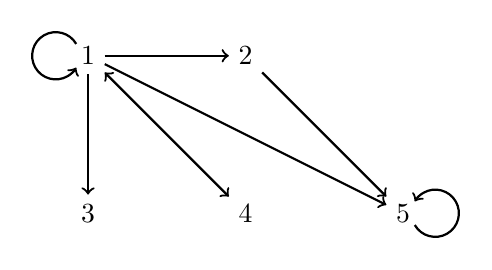
\begin{tikzpicture}
\node (atom1) at (0,2) {1};
\node (atom2) at (2,2) {2};
\node (atom4) at (0,0) {3};
\node (atom5) at (2,0) {4};
\node (atom6) at (4,0) {5};
\draw[->, thick] (atom1)+(-0.15,0.15) arc (-330:-30:.3); 
\draw[->, thick] (atom6)+(0.15,-0.15) arc (-150:150:.3); 
\draw[->, thick] (atom1) -- (atom2);
\draw[->, thick] (atom1) -- (atom4);
\draw[<->, thick] (atom1) -- (atom5);
\draw[->, thick] (atom1) -- (atom6);
\draw[->, thick] (atom2) -- (atom6);
\end{tikzpicture}
\end{center}
Determine whether each of the following sentences is true or false in that interpretation:
\begin{earg}
\item $\exists x\,\atom{R}{x,x}$ \hfill \myanswer{True}
\item $\forall x\,\atom{R}{x,x}$ \hfill \myanswer{False}
\item $\exists x \forall y\,\atom{R}{x,y}$ \hfill \myanswer{True}
\item $\exists x \forall y\,\atom{R}{y,x}$ \hfill \myanswer{False}
\item $\forall x \forall y \forall z ((\atom{R}{x,y} \eand \atom{R}{y,z}) \eif \atom{R}{x,z})$ \hfill \myanswer{False}
\item $\forall x \forall y \forall z ((\atom{R}{x,y} \eand \atom{R}{x,z}) \eif \atom{R}{y,z})$ \hfill \myanswer{False}
\item $\exists x \forall y \enot \atom{R}{x,y}$ \hfill \myanswer{True}
\item $\forall x(\exists y\,\atom{R}{x,y} \eif \exists y\,\atom{R}{y,x})$ \hfill \myanswer{True}
\item $\exists x \exists y (\enot x = y \eand \atom{R}{x,y} \eand \atom{R}{y,x})$ \hfill \myanswer{True}
\item $\exists x \forall y(\atom{R}{x,y} \eiff x = y)$ \hfill \myanswer{True}
\item $\exists x \forall y(\atom{R}{y,x} \eiff x = y)$ \hfill \myanswer{False}
\item $\exists x \exists y(\enot x = y \eand \atom{R}{x,y} \eand \forall z(\atom{R}{z,x} \eiff y = z))$ \hfill \myanswer{True}
\end{earg}

\setcounter{chapter}{29}
\chapter{Using Interpretations}\setcounter{ProbPart}{0}

\solutions
\problempart
\label{pr.Contingent}
Show that each of the following is neither a logical truth nor a contradiction:
\begin{earg}
\item \leftsolutions\ $\atom{D}{a} \eand \atom{D}{b}$
\item \leftsolutions\ $\exists x\,\atom{T}{x,h}$
\item \leftsolutions\ $\atom{P}{m} \eand \enot\forall x\,\atom{P}{x}$
\item $\forall z\, \atom{J}{z} \eiff \exists y\,\atom{J}{y}$
\item $\forall x (\atom{W}{x,m,n} \eor \exists y\atom{L}{x,y})$
\item $\exists x (\atom{G}{x} \eif \forall y\,\atom{M}{y})$
\item $\exists x (x = h \eand x = i)$
\end{earg}

\solutions
\problempart
\label{pr.NotEquiv}
Show that the following pairs of sentences are not logically equivalent.
\begin{earg}
\item $\atom{J}{a}$, $\atom{K}{a}$
\item $\exists x\,\atom{J}{x}$, $\atom{J}{m}$
\item $\forall x\,\atom{R}{x,x}$, $\exists x\,\atom{R}{x,x}$
\item $\exists x\,\atom{P}{x} \eif \atom{Q}{c}$, $\exists x (\atom{P}{x} \eif \atom{Q}{c})$
\item $\forall x(\atom{P}{x} \eif \enot \atom{Q}{x})$, $\exists x(\atom{P}{x} \eand \enot \atom{Q}{x})$
\item $\exists x(\atom{P}{x} \eand \atom{Q}{x})$, $\exists x(\atom{P}{x} \eif \atom{Q}{x})$
\item $\forall x(\atom{P}{x}\eif \atom{Q}{x})$, $\forall x(\atom{P}{x} \eand \atom{Q}{x})$
\item $\forall x\exists y\,\atom{R}{x,y}$, $\exists x\forall y\,\atom{R}{x,y}$
\item $\forall x\exists y\,\atom{R}{x,y}$, $\forall x\exists y\,\atom{R}{y,x}$
\end{earg}


\problempart
Show that the following sentences are jointly consistent:
\begin{earg}
\item $\atom{M}{a}, \enot \atom{N}{a}, Pa, \enot \atom{Q}{a}$
\item $\atom{L}{e,e}, \atom{L}{e,g}, \enot \atom{L}{g,e}, \enot \atom{L}{g,g}$
\item $\enot (\atom{M}{a} \eand \exists x\,\atom{A}{x}), Ma \eor \atom{F}{a}, \forall x(\atom{F}{x} \eif \atom{A}{x})$
\item $\atom{M}{a} \eor \atom{M}{b}, \atom{M}{a} \eif \forall x \enot \atom{M}{x}$
\item $\forall y\,\atom{G}{y}, \forall x (\atom{G}{x} \eif \atom{H}{x}), \exists y \enot \atom{I}{y}$
\item $\exists x(\atom{B}{x} \eor \atom{A}{x}), \forall x \enot \atom{C}{x}, \forall x\bigl[(\atom{A}{x} \eand \atom{B}{x}) \eif Cx\bigr]$
\item $\exists x\,\atom{X}{x}, \exists x\,\atom{Y}{x}, \forall x(\atom{X}{x} \eiff \enot \atom{Y}{x})$
\item $\forall x(\atom{P}{x} \eor \atom{Q}{x}), \exists x\enot(\atom{Q}{x} \eand \atom{P}{x})$
\item $\exists z(\atom{N}{z} \eand \atom{O}{z,z}), \forall x\forall y(\atom{O}{x,y} \eif \atom{O}{y,x})$
\item $\enot \exists x \forall y\,\atom{R}{x,y}, \forall x \exists y\,\atom{R}{x,y}$
\item $\enot \atom{R}{a,a}$, $\forall x (x=a \eor \atom{R}{x,a})$
\item $\forall x\forall y\forall z[(x=y \eor y=z )\eor x=z]$, $\exists x\exists y\ \enot x= y$
\item $\exists x\exists y((\atom{Z}{x} \eand \atom{Z}{y} )\eand x=y)$, $\enot \atom{Z}{d}$, $d=e$
\end{earg}

\problempart
Show that the following arguments are invalid:
\begin{earg}
\item $\forall x(\atom{A}{x} \eif \atom{B}{x}) \therefore \exists x\,\atom{B}{x}$
\item $\forall x(\atom{R}{x} \eif \atom{D}{x}), \forall x(\atom{R}{x} \eif \atom{F}{x}) \therefore \exists x(\atom{D}{x} \eand \atom{F}{x})$
\item $\exists x(\atom{P}{x}\eif \atom{Q}{x}) \therefore \exists x\,\atom{P}{x}$
\item $\atom{N}{a} \eand \atom{N}{b} \eand \atom{N}{c} \therefore \forall x\,\atom{N}{x}$
\item $\atom{R}{d,e}, \exists x\,\atom{R}{xd} \therefore \atom{R}{e,d}$
\item $\exists x(\atom{E}{x} \eand \atom{F}{x}), \exists x\,\atom{F}{x} \eif \exists x\,\atom{G}{x} \therefore \exists x(\atom{E}{x} \eand \atom{G}{x})$
\item $\forall x\,\atom{O}{x,c}, \forall x\,\atom{O}{c,x} \therefore \forall x\,\atom{O}{x,x}$
\item $\exists x(\atom{J}{x} \eand \atom{K}{x}), \exists x \enot \atom{K}{x}, \exists x \enot \atom{J}{x} \therefore \exists x(\enot \atom{J}{x} \eand \enot \atom{K}{x})$
\item $\atom{L}{a,b} \eif \forall x\,\atom{L}{x,b}, \exists x\,\atom{L}{x,b} \therefore \atom{L}{b,b}$
\item $\forall x(\atom{D}{x} \eif \exists y\,\atom{T}{y,x}) \therefore \exists y \exists z\ \enot y= z$
\end{earg}

%!TEX root = forallxsol.tex
%\part{Natural deduction for FOL}
%\label{ch.NDFOL}
%\addtocontents{toc}{\protect\mbox{}\protect\hrulefill\par}

\setcounter{chapter}{31}
\chapter{Basic rules for FOL}\setcounter{ProbPart}{0}
\problempart
The following two `proofs' are \emph{incorrect}. Explain why both are incorrect. Also, provide interpretations which would invalidate the fallacious argument forms the `proofs' enshrine:
\begin{multicols}{2}
	\begin{proof}
		\hypo{Rxx}{\forall x Rxx}
		\have{Raa}{Raa}\Ae{Rxx}
		\have{Ray}{\forall y Ray}\Ai{Raa}
		\have{Rxy}{\forall x \forall y Rxy}\Ai{Ray}
	\end{proof}
\vfill
\noindent\myanswer{When using $\forall$I, you must replace \emph{all} names with the new variable. So line 3 is bogus. As a counterinterpretation, consider the following:
\begin{center}
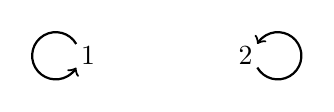
\begin{tikzpicture}
\node (atom4) at (0,0) {1};
\node (atom5) at (2,0) {2};
\draw[->, thick] (atom4)+(-0.15,0.15) arc (-330:-30:.3); 
\draw[->, thick] (atom5)+(0.15,-0.15) arc (-150:150:.3); 
\end{tikzpicture}
\end{center}}
\columnbreak
	\begin{proof}
		\hypo{AE}{\forall x \exists y Rxy}
		\have{E}{\exists y Ray}\Ae{AE}
		\open
			\hypo{ass}{Raa}
			\have{Ex}{\exists x Rxx}\Ei{ass}
		\close
		\have{con}{\exists x Rxx}\Ee{E, ass-Ex}
	\end{proof}
\vfill
\noindent\myanswer{The instantiating constant, `$a$', occurs in the line (line 2) to which $\exists$E is to be applied on line 5. So the use of $\exists$E on line 5 is bogus. As a counterinterpretation, consider the following:
\begin{center}
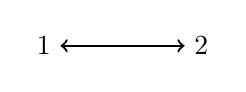
\begin{tikzpicture}
\node (atom4) at (0,0) {1};
\node (atom5) at (2,0) {2};
\draw[<->, thick] (atom4)--(atom5);
\end{tikzpicture}
\end{center}}
\end{multicols}


\problempart 
\label{pr.justifyFOLproof}
The following three proofs are missing their citations (rule and line numbers). Add them, to turn them into bona fide proofs. 
\begin{multicols}{2}
\begin{proof}
\hypo{p1}{\forall x\exists y(Rxy \eor Ryx)}
\hypo{p2}{\forall x\enot Rmx}
\have{3}{\exists y(Rmy \eor Rym)}\Ae{p1}
	\open
		\hypo{a1}{Rma \eor Ram}
		\have{a2}{\enot Rma}\Ae{p2}
		\have{a3}{Ram}\ds{a1, a2}
		\have{a4}{\exists x Rxm}\Ei{a3}
	\close
\have{n}{\exists x Rxm}\Ee{3, a1-a4}
\end{proof}

\begin{proof}
\hypo{1}{\forall x(\exists yLxy \eif \forall zLzx)}
\hypo{2}{Lab}
\have{3}{\exists y Lay \eif \forall zLza}\Ae{1}
\have{4}{\exists y Lay}\Ei{2}
\have{5}{\forall z Lza}\ce{3, 4}
\have{6}{Lca}\Ae{5}
\have{7}{\exists y Lcy \eif \forall zLzc}\Ae{1}
\have{8}{\exists y Lcy}\Ei{6}
\have{9}{\forall z Lzc}\ce{7, 8}
\have{10}{Lcc}\Ae{9}
\have{11}{\forall x Lxx}\Ai{10}
\end{proof}

\begin{proof}
\hypo{a}{\forall x(Jx \eif Kx)}
\hypo{b}{\exists x\forall y Lxy}
\hypo{c}{\forall x Jx}
\open
	\hypo{2}{\forall y Lay}
	\have{3}{Laa}\Ae{2}
	\have{d}{Ja}\Ae{c}
	\have{e}{Ja \eif Ka}\Ae{a}
	\have{f}{Ka}\ce{e, d}
	\have{4}{Ka \eand Laa}\ai{f, 3}
	\have{5}{\exists x(Kx \eand Lxx)}\Ei{4}
\close
\have{j}{\exists x(Kx \eand Lxx)}\Ee{b, 2-5}
\end{proof}
\end{multicols}


\problempart
\label{pr.BarbaraEtc.proof1}
In \S\ref{s:MoreMonadic} problem part A, we considered fifteen syllogistic figures of Aristotelian logic. Provide proofs for each of the argument forms. NB: You will find it \emph{much} easier if you symbolize (for example) `No F is G' as `$\forall x (Fx \eif \enot Gx)$'.
\\\myanswer{I shall prove the four Figure I syllogisms; the rest are \emph{extremely} similar.
\begin{multicols}{2}
\noindent \textbf{Barbara}
\begin{proof}
\hypo{gf}{\forall x (Gx \eif Fx)}
\hypo{hg}{\forall x (Hx \eif Gx)}
\have{gafa}{Ga \eif Fa}\Ae{gf}
\have{haga}{Ha \eif Ga}\Ae{hg}
\open
	\hypo{ha}{Ha}
	\have{ga}{Ga}\ce{haga, ha}
	\have{fa}{Fa}\ce{gafa, ga}
\close
\have{hafa}{Ha \eif Fa}\ci{ha-fa}
\have{con}{\forall x (Hx \eif Fx)}\Ai{hafa}
\end{proof}
\vfill
\noindent\textbf{Celerant} is exactly as Barbara, replacing `$F$' with `$\enot F$' throughout.
\columnbreak
\\\textbf{Ferio} 
\begin{proof}
\hypo{gnf}{\forall x (Gx \eif \enot Fx)}
\hypo{hg}{\exists x (Hx \eand  Gx)}
\open
	\hypo{haga}{Ha \eand Ga}
	\have{ha}{Ha}\ae{haga}
	\have{ga}{Ga}\ae{haga}
	\have{ganfa}{Ga \eif \enot Fa}\Ae{gnf}
	\have{nfa}{\enot Fa}\ce{ganfa, ga}
	\have{hanfa}{Ha \eand \enot Fa}\ai{ha, nfa}
	\have{hnf}{\exists x (Hx \eand \enot Fx)}\Ei{hanfa}
\close
\have{con}{\exists x (Hx \eand \enot Fx)}\Ee{hg, haga-hnf}
\end{proof}
\\\textbf{Darii} is exactly as Ferio, replacing `$\enot F$' with `$F$' throughout.\end{multicols}}

\

\problempart
\label{pr.BarbaraEtc.proof2}
Aristotle and his successors identified other syllogistic forms which depended upon `existential import'. Symbolize each of the following argument forms in FOL and offer proofs.
\begin{ebullet}
\newpage	\item \textbf{Barbari.} Something is H. All G are F. All H are G. So: Some H is F
	\\\myanswer{$\exists x Hx, \forall x(Gx \eif Fx), \forall x (Hx \eif Gx) \therefore \exists x (Hx \eand Fx)$
\begin{proof}
\hypo{imp}{\exists x Hx}
\hypo{gf}{\forall x (Gx \eif Fx)}
\hypo{hg}{\forall x (Hx \eif Gx)}
\open
	\hypo{ha}{Ha}
	\have{haga}{Ha \eif Ga}\Ae{hg}
	\have{ga}{Ga}\ce{haga, ha}
	\have{gafa}{Ga \eif Fa}\Ae{gf}
	\have{fa}{Fa}\ce{gafa, ga}
	\have{hafa}{Ha \eand Fa}\ai{ha, fa}
	\have{hf}{\exists x (Hx \eand Fx)}\Ei{hafa}
\close
\have{con}{\exists x (Hx \eand Fx)}\Ee{imp, ha-hf}
\end{proof}}
	
	\item \textbf{Celaront.} Something is H. No G are F. All H are G. So: Some H is not F
	\\\myanswer{$\exists x Hx, \forall x(Gx \eif \enot Fx), \forall x (Hx \eif Gx) \therefore \exists x (Hx \eand \enot Fx)$
\\	Proof is exactly as for Barbari, replacing `$F$' with `$\enot F$' throughout.}
	\item \textbf{Cesaro.} Something is H. No F are G. All H are G. So: Some H is not F.
	\\\myanswer{$\exists x Hx, \forall x(Fx \eif \enot Gx), \forall x (Hx \eif Gx) \therefore \exists x (Hx \eand \enot Fx)$
\begin{proof}
\hypo{imp}{\exists x Hx}
\hypo{fg}{\forall x (Fx \eif \enot Gx)}
\hypo{hng}{\forall x (Hx \eif  Gx)}
\open
	\hypo{ha}{Ha}
	\have{hanga}{Ha \eif Ga}\Ae{hng}
	\have{nga}{Ga}\ce{hanga, ha}
	\have{faga}{Fa \eif \enot Ga}\Ae{fg}
	\open
		\hypo{fa}{Fa}
		\have{ga}{\enot Ga}\ce{faga, fa}
		\have{red}{\ered}\ri{nga, ga}
	\close
	\have{nfa}{\enot Fa}\ni{fa-red}
	\have{hanfa}{Ha \eand \enot Fa}\ai{ha, nfa}
	\have{hnf}{\exists x (Hx \eand \enot Fx)}\Ei{hanfa}
\close
\have{con}{\exists x (Hx \eand \enot Fx)}\Ee{imp, ha-hnf}
\end{proof}
}
\newpage	\item \textbf{Camestros.} Something is H. All F are G. No H are G. So: Some H is not F.
	\\\myanswer{$\exists x Hx, \forall x(Fx \eif Gx), \forall x (Hx \eif \enot Gx) \therefore \exists x (Hx \eand \enot Fx)$
\begin{proof}
\hypo{imp}{\exists x Hx}
\hypo{fg}{\forall x (Fx \eif Gx)}
\hypo{hng}{\forall x (Hx \eif \enot Gx)}
\open
	\hypo{ha}{Ha}
	\have{hanga}{Ha \eif \enot Ga}\Ae{hng}
	\have{nga}{\enot Ga}\ce{hanga, ha}
	\have{faga}{Fa \eif Ga}\Ae{fg}
	\have{nfa}{\enot Fa}\mt{faga, nga}
	\have{hanfa}{Ha \eand \enot Fa}\ai{ha, nfa}
	\have{hnf}{\exists x (Hx \eand \enot Fx)}\Ei{hanfa}
\close
\have{con}{\exists x (Hx \eand \enot Fx)}\Ee{imp, ha-hnf}
\end{proof}}

	\item \textbf{Felapton.} Something is G. No G are F. All G are H. So: Some H is not F.
	\\\myanswer{$\exists x Gx, \forall x (Gx \eif \enot Fx), \forall x(Gx \eif Hx) \therefore \exists x (Hx \eand \enot Fx)$
\begin{proof}
\hypo{imp}{\exists x Gx}
\hypo{gnf}{\forall x (Gx \eif \enot Fx)}
\hypo{gh}{\forall x (Gx \eif Hx)}
\open
	\hypo{ga}{Ga}
	\have{gaha}{Ga \eif Ha}\Ae{gh}
	\have{ha}{Ha}\ce{gaha, ga}
	\have{ganfa}{Ga \eif \enot Fa}\Ae{gnf}
	\have{nfa}{\enot Fa}\ce{ganfa, ga}
	\have{hanfa}{Ha \eand \enot Fa}\ai{ha, nfa}
	\have{hnf}{\exists x (Hx \eand \enot Fx)}\Ei{hanfa}
\close
\have{con}{\exists x (Hx \eand Fx)}\Ee{imp, ga-hnf}
\end{proof}}
	\item \textbf{Darapti.} Something is G. All G are F. All G are H. So: Some H is F.
	\\\myanswer{$\exists x Gx, \forall x (Gx \eif Fx), \forall x(Gx \eif Hx) \therefore \exists x (Hx \eand Fx)$\\
	Proof is exactly as for Felapton, replacing `$\enot F$' with `$F$' throughout.}

\newpage	\item \textbf{Calemos.} Something is H. All F are G. No G are H. So: Some H is not F.
	\\\myanswer{$\exists x Hx, \forall x(Fx \eif Gx), \forall x(Gx \eif \enot Hx) \therefore \exists x (Hx \eand \enot Fx)$
\begin{proof}
\hypo{imp}{\exists x Hx}
\hypo{fg}{\forall x (Fx \eif Gx)}
\hypo{gnh}{\forall x (Gx \eif \enot Hx)}
\open
	\hypo{ha}{Ha}
	\have{ganha}{Ga \eif \enot Ha}\Ae{gnh}
	\open
		\hypo{ga}{Ga}
		\have{nha}{\enot Ha}\ce{ganha, ga}
		\have{red}{\ered}\ri{ha, nha}
	\close
	\have{nga}{\enot Ga}\ni{ga-red}
	\have{faga}{Fa \eif Ga}\Ae{fg}
	\have{nfa}{\enot Fa}\mt{faga, nga}
	\have{hanfa}{Ha \eand \enot Fa}\ai{ha, nfa}
	\have{hnf}{\exists x (Hx \eand Fx)}\Ei{hanfa}
\close
\have{con}{\exists x (Hx \eand Fx)}\Ee{imp, ha-hnf}
\end{proof}}
	
	\item \textbf{Fesapo.} Something is G. No F is G. All G are H. So: Some H is not F.
	\\\myanswer{$\exists x Gx, \forall x(Fx \eif \enot Gx), \forall x(Gx \eif Hx) \therefore \exists x (Hx \eand \enot Fx)$
	\begin{proof}
\hypo{imp}{\exists x Gx}
\hypo{fng}{\forall x (Fx \eif \enot Gx)}
\hypo{gh}{\forall x (Gx \eif Hx)}
\open
	\hypo{ga}{Ga}
	\have{gaha}{Ga \eif  Ha}\Ae{gh}
	\have{ha}{Ha}\ce{gaha, ga}
	\have{fanga}{Fa \eif \enot Ga}\Ae{fng}
	\open
		\hypo{fa}{Fa}
		\have{nga}{\enot Ga}\ce{fanga, fa}
		\have{red}{\ered}\ri{ga, nga}
	\close
	\have{nfa}{\enot Fa}\ni{fa-red}
	\have{hanfa}{Ha \eand \enot Fa}\ai{ha, nfa}
	\have{hnf}{\exists x (Hx \eand Fx)}\Ei{hanfa}
\close
\have{con}{\exists x (Hx \eand Fx)}\Ee{imp, ga-hnf}
\end{proof}}

\newpage	\item \textbf{Bamalip.} Something is F. All F are G. All G are H. So: Some H are F.
	\\\myanswer{$\exists x Fx, \forall x(Fx \eif Gx), \forall x(Gx \eif Hx) \therefore \exists x (Hx \eand Fx)$
\begin{proof}
\hypo{imp}{\exists x Fx}
\hypo{fg}{\forall x (Fx \eif Gx)}
\hypo{gh}{\forall x (Gx \eif Hx)}
\open
	\hypo{fa}{Fa}
	\have{faga}{Fa \eif Ga}\Ae{fg}
	\have{ga}{Ga}\ce{faga, fa}
	\have{gaha}{Ga \eif Ha}\Ae{gh}
	\have{ha}{Ha}\ce{gaha, ga}
	\have{hafa}{Ha \eand Fa}\ai{ha, fa}
	\have{hf}{\exists x (Hx \eand Fx)}\Ei{hafa}
\close
\have{con}{\exists x (Hx \eand Fx)}\Ee{imp, fa-hf}
\end{proof}}
\end{ebullet}

\problempart
\label{pr.someFOLproofs}
Provide a proof of each claim.
\begin{earg}
\item $\proves \forall x Fx \eor \enot \forall x Fx$
\myanswer{\begin{proof}
\open
	\hypo{Af}{\forall x Fx}
	\have{con}{\forall x Fx \eor \enot \forall x Fx}\oi{Af}
\close
\open
	\hypo{nAf}{\enot \forall x Fx}
	\have{con1}{\forall x Fx \eor \enot \forall x Fx}\oi{nAf}
\close
\have{con2}{\forall x Fx \eor \enot \forall x Fx}\tnd{Af-con, nAf-con1}
\end{proof}}
\item $\proves\forall z (Pz \eor \enot Pz)$
\myanswer{\begin{proof}
\open
	\hypo{Pa}{Pa}
	\have{con}{Pa \eor \enot Pa}\oi{Pa}
\close
\open
	\hypo{nPa}{\enot Pa}
	\have{con1}{Pa \eor \enot Pa}\oi{nPa}
\close
\have{con2}{Pa \eor \enot Pa}\tnd{Pa-con, nPa-con1}
\have{done}{\forall x(Px \eor \enot Px)}\Ai{con2}
\end{proof}}

\item $\forall x(Ax\eif Bx), \exists x Ax \proves \exists x Bx$
\myanswer{\begin{proof}
\hypo{Aab}{\forall x (Ax \eif Bx)}
\hypo{Ea}{\exists x Ax}
\open
	\hypo{a}{Aa}
	\have{ab}{Aa \eif Ba}\Ae{Aab}
	\have{b}{Ba}\ce{ab, a}
	\have{Eb}{\exists x Bx}\Ei{b}
\close
\have{Eb1}{\exists x Bx}\Ee{Ea, a-Eb}
\end{proof}}

\newpage\item $\forall x(Mx \eiff Nx), Ma\eand\exists x Rxa\proves \exists x Nx$
\myanswer{\begin{proof}
\hypo{Amn}{\forall x (Mx \eiff Nx)}
\hypo{mEr}{Ma \eand \exists x Rxa}
\have{m}{Ma}\ae{mEr}
\have{mn}{Ma \eiff Na}\Ae{Amn}
\have{n}{Na}\be{mn, m}
\have{En}{\exists x Nx}\Ei{n}
\end{proof}}

\item $\forall x \forall y Gxy\proves\exists x Gxx$
\myanswer{\begin{proof}
\hypo{AAg}{\forall x \forall y Gxy}
\have{Ag}{\forall y Gay}\Ae{AAg}
\have{g}{Gaa}\Ae{Ag}
\have{Eg}{\exists x Gxx}\Ei{g}
\end{proof}}

\item $\proves\forall x Rxx\eif \exists x \exists y Rxy$
\myanswer{\begin{proof}
\open
	\hypo{Ar}{\forall x Rxx}
	\have{r}{Raa}\Ae{Ar}
	\have{Er}{\exists y Ray}\Ei{r}
	\have{EEr}{\exists x \exists y Rxy}\Ei{Er}
\close
\have{ArEEr}{\forall x Rxx \eif \exists x \exists y Rxy}\ci{Ar-EEr}
\end{proof}}

\item $\proves\forall y \exists x (Qy \eif Qx)$
\myanswer{\begin{proof}
\open
	\hypo{q}{Qa}
	\have{q1}{Qa}\by{R}{q}
\close
\have{qq}{Qa \eif Qa}\ci{q-q1}
\have{Eqq}{\exists x(Qa \eif Qx)}\Ei{qq}
\have{AEqq}{\forall y \exists x(Qy \eif Qx)}\Ai{Eqq}
\end{proof}}


\item $Na \eif \forall x(Mx \eiff Ma), Ma, \enot Mb\proves \enot Na$
\myanswer{\begin{proof}
\hypo{nAmm}{Na \eif \forall x(Mx \eiff Ma)}
\hypo{m}{Ma}
\hypo{nm}{\enot Mb}
\open
	\hypo{n}{Na}
	\have{Amm}{\forall x (Mx \eiff Ma)}\ce{nAmm, n}
	\have{mm}{Mb \eiff Ma}\Ae{Amm}
	\have{mb}{Mb}\be{mm, m}
	\have{red}{\ered}\ri{mb, nm}
\close
\have{nn}{\enot Na}\ni{n-red}
\end{proof}}

\newpage\item $\forall x \forall y (Gxy \eif Gyx) \proves \forall x\forall y (Gxy \eiff Gyx)$
\myanswer{\begin{proof}
\hypo{AAgg}{\forall x \forall y(Gxy \eif Gyx)}
\open
	\hypo{gab}{Gab}
	\have{Agg}{\forall y(Gay \eif Gya)}\Ae{AAgg}
	\have{gg}{Gab \eif Gba}\Ae{Agg}
	\have{gba}{Gba}\ce{gg, gab}
\close
\open
	\hypo{gba1}{Gba}
	\have{Agg1}{\forall y(Gby \eif Gyb)}\Ae{AAgg}
	\have{gg1}{Gba \eif Gab}\Ae{Agg1}
	\have{gab1}{Gab}\ce{gg1, gba1}
\close
\have{bi}{Gab \eiff Gba}\bi{gab-gba, gba1-gab1}
\have{Abi}{\forall y(Gay \eiff Gya)}\Ai{bi}
\have{AAbi}{\forall x \forall y (Gxy \eiff Gyx)}\Ai{Abi}
\end{proof}}

\item $\forall x(\enot Mx \eor Ljx), \forall x(Bx\eif Ljx), \forall x(Mx\eor Bx)\proves \forall xLjx$
\myanswer{\begin{proof}
\hypo{Anmlj}{\forall x (\enot Mx \eor Ljx)}
\hypo{Ablj}{\forall x (Bx \eif Ljx)}
\hypo{Amb}{\forall x (Mx \eor Bx)}
\have{nmlj}{\enot Ma \eor Ljx}\Ae{Anmlj}
\have{blj}{Ba \eif Lja}\Ae{Ablj}
\have{mb}{Ma \eor Ba}\Ae{Amb}
\open
	\hypo{nm}{\enot Ma}
	\have{b}{Ba}\ds{mb, nm}
	\have{lj}{Lja}\ce{blj, b}
\close
\open
	\hypo{lj1}{Lja}
	\have{lj2}{Lja}\by{R}{lj1}
\close
\have{lj3}{Lja}\oe{nmlj, nm-lj, lj1-lj2}
\have{Alj}{\forall x Ljx}\Ai{lj3}
\end{proof}}
\end{earg}

\solutions
\problempart
\label{pr.likes}
Write a symbolization key for the following argument, symbolize it, and prove it:
\begin{quote}
There is someone who likes everyone who likes everyone that she likes. Therefore, there is someone who likes herself.
\end{quote}
\myanswer{Symbolization key:
\begin{ekey}
\item[\text{domain}] all people
\item[Lxy] \gap{x} likes \gap{y}
\end{ekey}
$\exists x \forall y(\forall z(Lxz \eif Lyz) \eif Lxy) \therefore \exists x  Lxx$
\begin{proof}
\hypo{1}{\exists x\forall y(\forall z(Lxz \eif Lyz) \eif Lxy)}
\open
	\hypo{a}{\forall y(\forall z(Laz \eif Lyz) \eif Lay)}
	\have{b}{\forall z(Laz \eif Laz) \eif Laa} \Ae{a}
	\open
		\hypo{lac}{Lac}
		\have{lac1}{Lac}\by{R}{lac}
	\close
	\have{laclac}{Lac \eif Lac}\ci{lac-lac1}
	\have{Alaz}{\forall z (Laz \eif Laz)}\Ai{laclac}
	\have{laa}{Laa}\ce{b, Alaz}
	\have{El}{\exists x Lxx}\Ei{laa}
\close
\have{n}{\exists x Lxx} \Ee{1, a--El}
\end{proof}}

\problempart
Show that each pair of sentences is provably equivalent.
\begin{earg}
\item $\forall x (Ax\eif \enot Bx)$, $\enot\exists x(Ax \eand Bx)$
\item $\forall x (\enot Ax\eif Bd)$, $\forall x Ax \eor Bd$
\item $\exists x Px \eif Qc$, $\forall x (Px \eif Qc)$
\end{earg}


\solutions
\setcounter{ProbPart}{7} % next exercise is H (= 8)
\problempart
\label{pr.FOLequivornot}
For each of the following pairs of sentences: if they are provably equivalent, give proofs to show this. If they are not, construct an interpretation to show that they are not logically equivalent.
\begin{earg}
\item $\forall x Px \eif Qc, \forall x (Px \eif Qc)$ \hfill \myanswer{Not logically equivalent}
\\\myanswer{Counter-interpretation: let the domain be the numbers $1$ and $2$. Let `$c$' name $1$. Let `$Px$' be true of and only of $1$. Let `$Qx$' be true of, and only of, $2$.}
\item $\forall x\forall y \forall z Bxyz, \forall x Bxxx$\hfill \myanswer{Not logically equivalent}
\\\myanswer{Counter-interpretation: let the domain be the numbers $1$ and $2$. Let `$Bxyz$' be true of, and only of, \ntuple{1,1,1} and \ntuple{2,2,2}.}
\item $\forall x\forall y Dxy, \forall y\forall x Dxy$ \hfill \myanswer{Provably equivalent\begin{multicols}{2}
\begin{proof}
\hypo{AAd}{\forall x \forall y Dxy}
\have{Ad}{\forall y Day}\Ae{AAd}
\have{A}{Dab}\Ae{Ad}
\have{Ad1}{\forall x Dxb}\Ai{A}
\have{AAd1}{\forall y \forall x Dxy}\Ai{Ad1}
\end{proof}
\begin{proof}
\hypo{AAd}{\forall y \forall x Dxy}
\have{Ad}{\forall x Dxa}\Ae{AAd}
\have{A}{Dba}\Ae{Ad}
\have{Ad1}{\forall y Dby}\Ai{A}
\have{AAd1}{\forall x \forall y Dxy}\Ai{Ad1}
\end{proof}
\end{multicols}}
\item $\exists x\forall y Dxy, \forall y\exists x Dxy$ \hfill \myanswer{Not logically equivalent}
\\\myanswer{Counter-interpretation: let the domain be the numbers $1$ and $2$. Let `$Dxy$' hold of and only of \ntuple{1,2} and \ntuple{2,1}. This is depicted thus:
\begin{center}
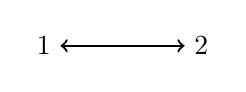
\begin{tikzpicture}
\node (atom4) at (0,0) {1};
\node (atom5) at (2,0) {2};
\draw[<->, thick] (atom4)--(atom5);
\end{tikzpicture}
\end{center}}
\item $\forall x (Rca \eiff Rxa), Rca \eiff \forall x Rxa$ \hfill \myanswer{Not logically equivalent}
\\\myanswer{Counter-interpretation, consider the following diagram, allowing `$a$' to name 1 and `$c$' to name 2:
\begin{center}
\begin{tikzpicture}
\node (atom4) at (0,0) {1};
\node (atom5) at (2,0) {2};
\draw[->, thick] (atom4)+(-0.15,0.15) arc (-330:-30:.3); 
%\draw[->, thick] (atom5)+(0.15,-0.15) arc (-150:150:.3); 
%\draw[<->, thick] (atom4)--(atom5);
\end{tikzpicture}
\end{center}}
\end{earg}

\solutions
\problempart
\label{pr.FOLvalidornot}
For each of the following arguments: If it is valid in FOL, give a proof. If it is invalid, construct an interpretation to show that it is invalid.
\begin{earg}
\item $\exists y\forall x Rxy \therefore \forall x\exists y Rxy$ \hfill \myanswer{Valid
\begin{proof}
\hypo{EAr}{\exists y \forall x Rxy}
\open
	\hypo{Ar}{\forall x Rxa}
	\have{r}{Rba}\Ae{Ar}
	\have{Er}{\exists y Rby}\Ei{r}
\close
\have{Er1}{\exists y Rby}\Ee{EAr, Ar-Er}
\have{AEr}{\forall x \exists y Rxy}\Ai{Er1}
\end{proof}}
\item $\exists x(Px \eand \enot Qx) \therefore \forall x(Px \eif \enot Qx)$ \hfill \myanswer{Not valid
\\Counter interpretation: let the domain be the numbers $1$ and $2$. Let `$Px$' be true of everything in the domain. Let `$Qx$' be true of, and only of, $2$.}
\item $\forall x(Sx \eif Ta), Sd \therefore Ta$ \hfill \myanswer{Valid
\begin{proof}
\hypo{Ast}{\forall x (Sx \eif Ta)}
\hypo{s}{Sd}
\have{st}{Sd \eif Ta}\Ae{Ast}
\have{t}{Ta}\ce{st, s}
\end{proof}}
\item $\forall x(Ax\eif Bx), \forall x(Bx \eif Cx) \therefore \forall x(Ax \eif Cx)$ \hfill \myanswer{Valid
\begin{proof}
\hypo{Aab}{\forall x (Ax \eif Bx)}
\hypo{Abc}{\forall x (Bx \eif Cx)}
\have{ab}{Aa \eif Ba}\Ae{Aab}
\have{bc}{Ba \eif Ca}\Ae{Abc}
\open
	\hypo{a}{Aa}
	\have{b}{Ba}\ce{ab, a}
	\have{c}{Ca}\ce{bc, b}
\close
\have{ac}{Aa \eif Ca}\ci{a-c}
\have{Aac}{\forall x (Ax \eif Cx)}\Ai{ac}
\end{proof}}
\item $\exists x(Dx \eor Ex), \forall x(Dx \eif Fx) \therefore \exists x(Dx \eand Fx)$ \hfill \myanswer{Invalid\\
Counter-interpretation: let the domain be the number $1$ . Let `$Dx$' hold of nothing. Let both `$Ex$' and `$Fx$' hold of everything.}
\item $\forall x\forall y(Rxy \eor Ryx) \therefore Rjj$ \hfill \myanswer{Valid
\begin{proof}
\hypo{AArr}{\forall x \forall y (Rxy \eor Ryx)}
\have{Arr}{\forall y (Rjy \eor Ryj)}\Ae{AArr}
\have{rr}{Rjj \eor Rjj}\Ae{Arr}
\open
	\hypo{r1}{Rjj}
	\have{r2}{Rjj}\by{R}{r1}
\close
\open
	\hypo{r3}{Rjj}
	\have{r4}{Rjj}\by{R}{r3}
\close
\have{r5}{Rjj}\oe{rr, r1-r2, r3-r4}
\end{proof}}

\item $\exists x\exists y(Rxy \eor Ryx) \therefore Rjj$ \hfill \myanswer{Invalid\\
Counter-interpretation: consider the following diagram, allowing `$j$' to name $2$.
\begin{center}
\begin{tikzpicture}
\node (atom4) at (0,0) {1};
\node (atom5) at (2,0) {2};
\draw[->, thick] (atom4)+(-0.15,0.15) arc (-330:-30:.3); 
%\draw[->, thick] (atom5)+(0.15,-0.15) arc (-150:150:.3); 
%\draw[<->, thick] (atom4)--(atom5);
\end{tikzpicture}
\end{center}}
\item $\forall x Px \eif \forall x Qx, \exists x \enot Px \therefore \exists x \enot Qx$ \hfill \myanswer{Invalid\\
Counter-interpretation: let the domain be the number $1$. Let `$Px$' be true of nothing. Let `$Qx$' be true of everything.}
\end{earg}

\problempart
Show that each of the following is provably inconsistent.
\begin{earg}
\item \{$Sa\eif Tm$, $Tm \eif Sa$, $Tm \eand \enot Sa$\}
\item \{$\enot\exists x Rxa$, $\forall x \forall y Ryx$\}
\item \{$\enot\exists x \exists y Lxy$, $Laa$\}
\item \{$\forall x(Px \eif Qx)$, $\forall z(Pz \eif Rz)$, $\forall y Py$, $\enot Qa \eand \enot Rb$\}
\end{earg}


\chapter{Conversion of quantifiers}\setcounter{ProbPart}{0}
\problempart
Show that the following are provably inconsistent:
\begin{earg}
\item $Sa\eif Tm, Tm \eif Sa, Tm \eand \enot Sa$
\myanswer{\begin{proof}
\hypo{st}{Sa \eif Tm}
\hypo{ts}{Tm \eif Sa}
\hypo{tns}{Tm \eand \enot Sa}
\have{t}{Tm}\ae{tns}
\have{ns}{\enot Sa}\ae{tns}
\have{s}{Sa}\ce{ts, t}
\have{red}{\ered}\ri{ns,s}
\end{proof}}
\item $\enot\exists x Rxa, \forall x \forall y Ryx$
\myanswer{\begin{proof}
\hypo{nEr}{\enot \exists x Rxa}
\hypo{AAr}{\forall x \forall y Ryx}
\have{Anr}{\forall x \enot Rxa}\cq{nEr}
\have{nr}{\enot Rba}\Ae{Anr}
\have{Ar}{\forall y Rya}\Ae{AAr}
\have{r}{Rba}\Ae{Ar}
\have{red}{\ered}\ri{r, nr}
\end{proof}}
\item $\enot\exists x \exists y Lxy, Laa$
\myanswer{\begin{proof}
\hypo{nEEl}{\enot \exists x \exists y Lxy}
\hypo{l}{Laa}
\have{AnEl}{\forall x \enot \exists y Lxy}\cq{nEEl}
\have{nEl}{\enot \exists y Lay}\Ae{AnEl}
\have{Anl}{\forall y \enot Lay}\cq{nEl}
\have{n}{\enot Laa}\Ae{Anl}
\have{red}{\ered}\ri{l,n}
\end{proof}}
\item $\forall x(Px \eif Qx), \forall z(Pz \eif Rz), \forall y Py, \enot Qa \eand \enot Rb$
\myanswer{\begin{proof}
\hypo{Apq}{\forall x(Px \eif Qx)}
\hypo{Apr}{\forall z(Pz \eif Rz)}
\hypo{Ap}{\forall y Py}
\hypo{nqnr}{\enot Qa \eand \enot Rb}
\have{nq}{\enot Qa}\ae{nqnr}
\have{pq}{Pa \eif Qa}\Ae{Apq}
\have{np}{\enot Pa}\mt{pq, nq}
\have{p}{Pa}\Ae{Ap}
\have{red}{\ered}\ri{p,np}
\end{proof}}
\end{earg}

\problempart
Show that each pair of sentences is provably equivalent: %TB: Again, have to do some manual numbering to make the multicols have enough space.

\

1.  $\forall x (Ax\eif \enot Bx), \enot\exists x(Ax \eand Bx)$
\myanswer{\begin{multicols}{2}
\begin{proof}
\hypo{Aanb}{\forall x (Ax \eif \enot Bx)}
\open
	\hypo{Eab}{\exists x (Ax \eand Bx)}
	\open
		\hypo{ab}{Aa \eand Ba}
		\have{a}{Aa}\ae{ab}
		\have{b}{Ba}\ae{ab}
		\have{anb}{Aa \eif \enot Ba}\Ae{Aanb}
		\have{nb}{\enot Ba}\ce{anb, a}
		\have{red}{\ered}\ri{b, nb}
	\close
	\have{red1}{\ered}\Ee{Eab, ab-red}
	\close
\have{nEab}{\enot \exists x(Ax \eand Bx)}\ni{Eab-red1}
\end{proof}
\begin{proof}
\hypo{nEab}{\enot \exists x(Ax \eand Bx)}
\have{Anab}{\forall x\enot(Ax \eand Bx)}\cq{nEab}
\have{nab}{\enot (Aa \eand Ba)}\Ae{Anab}
\open
	\hypo{a}{Aa}
	\open
		\hypo{b}{Ba}
		\have{ab}{Aa \eand Ba}\ai{a,b}
		\have{red}{\ered}\ri{ab,nab}
	\close
	\have{nb}{\enot Ba}\ni{b-red}
\close
\have{anb}{Aa \eif \enot Ba}\ci{a-nb}
\have{Aanb}{\forall x (Ax \eif \enot Bx)}\Ai{anb}		
\end{proof}
\end{multicols}}
2. $\forall x (\enot Ax\eif Bd), \forall x Ax \eor Bd$
\myanswer{\begin{multicols}{2}
\begin{proof}
\hypo{Anab}{\forall x(\enot Ax \eif Bd)}
\have{nab}{\enot Aa \eif Bd}\Ae{Anab}
\open
	\hypo{b}{Bd}
	\have{Aab}{\forall x Ax \eor Bd}\oi{ab}
\close
\open
	\hypo{nb}{\enot Bd}
	\have{nna}{\enot \enot Aa}\mt{nab, nb}
	\have{a}{Aa}\dne{nna}
	\have{Aa}{\forall x Ax}\Ae{a}
	\have{Aab1}{\forall x Ax \eor Bd}\oi{Aa}
\close
\have{Aab2}{\forall xAx \eor Bd}\tnd{b-Aab, nb-Aab1}
\end{proof}
\begin{proof}
\hypo{Aab}{\forall x Ax \eor Bd}
\open
	\hypo{na}{\enot Aa}
	\open
		\hypo{Aa}{\forall x Ax}
		\have{a}{Aa}\Ae{Aa}
		\have{red}{\ered}\ri{a, na}
	\close
	\have{nAa}{\enot \forall x Ax}\ni{Aa-red}
	\have{b}{Bd}\ds{Aab, nAa}
\close
\have{nab}{\enot Aa \eif Bd}\ci{na-b}
\have{Anab}{\forall x (Ax \eif Bd)}\Ai{nab}
\end{proof}
\end{multicols}}


\problempart
In \S\ref{s:MoreMonadic}, we considered what happens when we move quantifiers `across' various logical operators. Show that each pair of sentences is provably equivalent: %TB: Again, manual line numbering to give multicols enough space.

\

1.  $\forall x (Fx \eand Ga), \forall x Fx \eand Ga$ 
\myanswer{
\begin{multicols}{2}
\begin{proof}
\hypo{Afg}{\forall x (Fx \eand Ga)}
\have{fg}{Fb \eand Ga}\Ae{Afg}
\have{f}{Fb}\ae{fg}
\have{g}{Ga}\ae{ga}
\have{Af}{\forall x Fx}\Ai{f}
\have{Afg1}{\forall x Fx \eand Ga}\ai{Af, g}
\end{proof}
\begin{proof}
\hypo{Afg}{\forall x Fx \eand Ga}
\have{Af}{\forall x Fx}\ae{Afg}
\have{g}{Ga}\ae{Afg}
\have{f}{Fb}\Ae{Af}
\have{fg}{Fb \eand Ga}\ai{f, g}
\have{Afg1}{\forall x (Fx \eand Ga)}\Ai{fg}
\end{proof}
\end{multicols}}
2. $\exists x (Fx \eor Ga), \exists x Fx \eor Ga$
\myanswer{
\begin{multicols}{2}
\begin{proof}
\hypo{Efg}{\exists x (Fx \eor Ga)}
\open
	\hypo{fg}{Fb \eor Ga}
	\open
		\hypo{f}{Fb}
		\have{Ef}{\exists x Fx}\Ei{f}
		\have{Efg1}{\exists x Fx \eor Ga}\oi{Ef}
	\close
	\open
		\hypo{g}{Ga}
		\have{Efg2}{\exists x Fx \eor Ga}\oi{g}
	\close		
	\have{Efg3}{\exists x Fx \eor Ga}\oe{fg, f-Efg1, g-Efg2}
\close
\have{Efg4}{\exists x Fx \eor Ga}\Ee{Efg, fg-Efg3}
\end{proof}
\begin{proof}
\hypo{Efg}{\exists x Fx \eor Ga}
\open
	\hypo{Ef}{\exists x Fx}
	\open
		\hypo{f}{Fb}
		\have{fg}{Fb \eor Ga}\oi{f}
		\have{Efg1}{\exists x (Fx \eor Ga)}\Ei{fg}
	\close
	\have{Efg2}{\exists x (Fx \eor Ga)}\Ee{Ef, f-Efg1}
\close
\open
	\hypo{g}{Ga}
	\have{fbg}{Fb \eor Ga}\oi{g}
	\have{Efg3}{\exists x (Fx \eor Ga)}\Ei{fbg}
\close
\have{Efg4}{\exists x (Fx \eor Ga)}\oe{Efg, Ef-Efg2, g-Efg3}
\end{proof}
\end{multicols}}
3. $\forall x(Ga \eif Fx), Ga \eif \forall x Fx$
\myanswer{\begin{multicols}{2}
\begin{proof}
\hypo{Agf}{\forall x(Ga \eif Fx)}
\have{gf}{Ga \eif Fb}\Ae{Agf}
\open
	\hypo{g}{Ga}
	\have{f}{Fb}\ce{gf, g}
	\have{Af}{\forall x Fx}\Ai{f}
\close
\have{gAf}{Ga \eif \forall x Fx}\ci{g-Af}
\end{proof}
\begin{proof}
\hypo{gAf}{Ga \eif \forall x Fx}
\open
	\hypo{g}{Ga}
	\have{Af}{\forall x Fx}\ce{gAf, g}
	\have{f}{Fb}\Ae{Af}
\close
\have{gf}{Ga \eif Fb}\ci{g-f}
\have{Agf}{\forall x (Ga \eif Fx)}\Ai{gf}
\end{proof}
\end{multicols}}

4. $\forall x(Fx \eif Ga), \exists x Fx \eif Ga$
\myanswer{\begin{multicols}{2}
\begin{proof}
\hypo{Afg}{\forall x(Fx \eif Ga)}
\open
	\hypo{Ef}{\exists x Fx}
	\open
		\hypo{f}{Fb}
		\have{fg}{Fb \eif Ga}\Ae{Afg}
		\have{g}{Ga}\ce{fg, f}
	\close
	\have{g1}{Ga}\Ee{Ef, f-g}
\close
\have{Efg}{\exists x Fx \eif Ga}\ci{Ef-g1}	
\end{proof}
\begin{proof}
\hypo{Efg}{\exists x Fx \eif Ga}
\open
	\hypo{f}{Fb}
	\have{Ef}{\exists x Fx}\Ei{f}
	\have{g}{Ga}\ce{Efg, Ef}
\close
\have{fg}{Fb \eif Ga}\ci{f-g}
\have{Afg}{\forall x(Fx \eif Ga)}\Ai{fg}	
\end{proof}
\end{multicols}}
5. $\exists x(Ga \eif Fx), Ga \eif \exists x Fx$
\myanswer{\begin{multicols}{2}
\begin{proof}
\hypo{Egf}{\exists x(Ga \eif Fx)}
\open
	\hypo{g}{Ga}
	\open
		\hypo{gf}{Ga \eif Fb}
		\have{f}{Fb}\ce{gf, g}
		\have{Ef}{\exists x Fx}\Ei{f}
	\close
	\have{Ef1}{\exists x Fx}\Ee{Egf, gf-Ef}
\close
\have{gEf}{Ga \eif \exists x Fx}\ci{g-Ef1}
\end{proof}
\begin{proof}
\hypo{gEf}{Ga \eif \exists x Fx}
\open
	\hypo{g}{Ga}
	\have{Ef}{\exists x Fx}
	\open
		\hypo{f}{Fb}
		\open
			\hypo{g1}{Ga}
			\have{f1}{Fb}\by{R}{f}
		\close
		\have{gf}{Ga \eif Fb}\ci{g1-f1}
		\have{Egf}{\exists x(Ga \eif Fx)}\Ei{gf}
	\close
	\have{Egf1}{\exists x (Ga \eif Fx)}\Ee{Ef, f-Egf}
\close
\open
	\hypo{ng}{\enot Ga}
	\open
		\hypo{g2}{Ga}
		\have{red}{\ered}\ri{g2, ng}
		\have{f2}{Fb}\re{red}
	\close
	\have{gf1}{Ga \eif Fb}\ce{g2-f2}
	\have{Egf2}{\exists x (Ga \eif Fx)}\Ei{gf1}
\close
\have{con}{\exists x (Ga \eif Fx)}\tnd{g-Egf1, ng-Egf2}
\end{proof}
\end{multicols}}

6. $\exists x(Fx \eif Ga), \forall x Fx \eif Ga$
\myanswer{\begin{multicols}{2}
\begin{proof}
\hypo{Efg}{\exists x (Fx \eif Ga)}
\open
	\hypo{Af}{\forall x Fx}
	\open
		\hypo{fg}{Fb \eif Ga}
		\have{f}{Fb}\Ae{Af}
		\have{g}{Ga}\ce{fg,f}
	\close
	\have{g1}{Ga}\Ee{Efg, fg-g}
\close
\have{Afg}{\forall x Fx \eif Ga}\ci{Af-g1}
\end{proof}
\begin{proof}
\hypo{Afg}{\forall x Fx \eif Ga}
\open
	\hypo{Af}{\forall x Fx}
	\have{g}{Ga}\ce{Afg, Af}
	\open
		\hypo{f}{Fb}
		\have{g1}{Ga}\by{R}{g}
	\close
	\have{fg}{Fb \eif Ga}\ci{f-g1}
	\have{Efg}{\exists x (Fx \eif Ga)}\Ei{fg}
\close
\open
	\hypo{nAf}{\enot \forall x Fx}
	\have{Enf}{\exists x \enot Fx}\cq{nAf}
	\open
		\hypo{nf}{\enot Fb}
		\open
			\hypo{f1}{Fb}
			\have{red}{\ered}\ri{f1, nf}
			\have{g2}{Ga}\re{red}
		\close
		\have{fg1}{Fb \eif Ga}\ci{f1-g2}
		\have{Efg1}{\exists x (Fx \eif Ga)}\Ei{fg1}
	\close
	\have{Efg2}{\exists x (Fx \eif Ga)}\Ee{Enf, nf-Efg1}
\close
\have{Efg3}{\exists x (Fx \eif Ga)}\tnd{Af-Efg, nAf-Efg2}
\end{proof}
\end{multicols}}
NB: the variable `$x$' does not occur in `$Ga$'.

When all the quantifiers occur at the beginning of a sentence, that sentence is said to be in \emph{prenex normal form}. Together with the CQ rules, these equivalences are sometimes called \emph{prenexing rules}, since they give us a means for putting any sentence into prenex normal form.

\chapter{Rules for identity}\setcounter{ProbPart}{0}
\problempart
\label{pr.identity}
Provide a proof of each claim.
\begin{earg}
\item $Pa \eor Qb, Qb \eif b=c, \enot Pa \proves Qc$
\myanswer{
\begin{proof}
\hypo{pq}{Pa \eor Qb}
\hypo{qbi}{Qb \eif b=c}
\hypo{np}{\enot Pa}
\have{q}{Qb}\ds{pq, np}
\have{i}{b=c}\ce{qbi, q}
\have{qc}{Qc}\ie{i,q}
\end{proof}}
\item $m=n \eor n=o, An \proves Am \eor Ao$
\myanswer{
\begin{proof}
\hypo{mnino}{m=n \eor n=o}
\hypo{an}{An}
\open
	\hypo{min}{m=n}
	\have{am}{Am}\ie{min, an}
	\have{amao}{Am \eor Ao}\oi{am}
\close
\open
	\hypo{nio}{n=o}
	\have{ao}{Ao}\ie{nio, ao}
	\have{amao1}{Am \eor Ao}\oi{ao}
\close
\have{amao2}{Am \eor Ao}\oe{mnino, min-amao, nio-amao1}
\end{proof}}
\item $\forall x\ x=m, Rma\proves \exists x Rxx$
\myanswer{\begin{proof}
\hypo{Axim}{\forall x\ x=m}
\hypo{rma}{Rma}
\have{aim}{a=m}\Ae{Axim}
\have{raa}{Raa}\ie{aim, rma}
\have{Erxx}{\exists x Rxx}\Ei{raa}
\end{proof}}
\item $\forall x\forall y(Rxy \eif x=y)\proves Rab \eif Rba$
\myanswer{\begin{proof}
\hypo{AArxiy}{\forall x \forall y(Rxy \eif x = y)}
\open
	\hypo{rab}{Rab}
	\have{Araiy}{\forall y(Ray \eif a = y)}\Ae{AArxiy}
	\have{raib}{Rab \eif a=b}\Ae{Araiy}
	\have{aib}{a=b}\ce{raib, rab}
	\have{raa}{Raa}\ie{aib, rab}
	\have{rba}{Rba}\ie{aib, raa}
\close
\have{rabrba}{Rab \eif Rba}\ci{rab-rba}
\end{proof}}
\item $\enot \exists x\enot x = m \proves \forall x\forall y (Px \eif Py)$
\myanswer{\begin{proof}
\hypo{nEnxim}{\enot \exists x \enot x = m}
\have{Annxim}{\forall x \enot \enot x =m}\cq{nEnxim}
\have{nnaim}{\enot \enot a = m}\Ae{Annxim}
\have{aim}{a = m}\dne{nnaim}
\have{nnbim}{\enot \enot b = m}\Ae{Annxim}
\have{bim}{b = m}\dne{nnbim}
\open
	\hypo{pa}{Pa}
	\have{pm}{Pm}\ie{nnaim, pa}
	\have{pb}{Pb}\ie{nnbim, pm}
\close
\have{papb}{Pa \eif Pb}\ci{pa-pb}
\have{Apapy}{\forall y (Pa \eif Py)}\Ai{papb}
\have{AApxpy}{\forall x\forall y (Px \eif Py)}\Ai{Apapy}
\end{proof}}
\item $\exists x Jx, \exists x \enot Jx\proves \exists x \exists y\ \enot x = y$
\myanswer{\begin{proof}
\hypo{Ej}{\exists x Jx}
\hypo{Enj}{\exists x \enot Jx}
\open
	\hypo{j}{Ja}
	\open
		\hypo{nj}{\enot Jb}
		\open
			\hypo{aib}{a=b}
			\have{jb}{Jb}\ie{aib, j}
			\have{red}{\ered}\ri{jb, nj}
		\close
		\have{naib}{\enot a = b}\ni{aib-red}
		\have{Enaiy}{\exists y \enot a = y}\Ei{naib}
		\have{EEnxiy}{\exists x \exists y \enot x = y}\Ei{Enaiy}
	\close
	\have{EEnxiy1}{\exists x \exists y \enot x = y}\Ee{Enj, nj-EEnxiy}
\close
\have{EEnxiy2}{\exists x \exists y \enot x = y}\Ee{Ej, j-EEnxiy1}
\end{proof}}

\item $\forall x(x=n \eiff Mx), \forall x(Ox \eor \enot Mx)\proves On$
\myanswer{\begin{proof}
\hypo{Axinm}{\forall x(x = n \eiff Mx)}
\hypo{Aonm}{\forall x(Ox \eor \enot Mx)}
\have{ninm}{n = n \eiff Mn}\Ae{Axinm}
\have{nin}{n=n}\ii{}
\have{m}{Mn}\be{ninm,nin}
\have{onm}{On \eor \enot Mn}\Ae{Aonm}
\open
	\hypo{no}{\enot On}
	\have{nm}{\enot Mn}\ds{onm, no}
	\have{red}{\ered}\ri{m, nm}
\close
\have{nno}{\enot\enot On}\ni{no-red}
\have{o}{On}\dne{nno}
\end{proof}}

\item $\exists x Dx, \forall x(x=p \eiff Dx)\proves Dp$
\myanswer{\begin{proof}
\hypo{Ed}{\exists x Dx}
\hypo{Axd}{\forall x(x = p \eiff Dx)}
\open
	\hypo{d}{Dc}
	\have{cipd}{c = p \eiff Dc}\Ae{Axd}
	\have{cip}{c = p}\be{cipd, d}
	\have{dp}{Dp}\ie{cip, d}
\close
\have{dp1}{Dp}\Ee{Ed, d-dp}
\end{proof}}

\item $\exists x\bigl[(Kx \eand \forall y(Ky \eif x=y)) \eand Bx\bigr], Kd\proves Bd$
\myanswer{\begin{proof}
\hypo{EkAkb}{\exists x\bigl[(Kx \eand \forall y(Ky \eif x=y) \eand Bx\bigr]}
\hypo{kd}{Kd}
\open
	\hypo{kAkb}{(Ka \eand \forall y(Ky \eif a=y)) \eand Ba}
	\have{kAk}{Ka \eand \forall y(Ky \eif a=y)}\ae{kAkb}
	\have{k}{Ka}\ae{kAk}
	\have{Ak}{\forall y (Ky \eif a = y)}\ae{kAk}
	\have{kdaid}{Kd \eif a = d}\Ae{Ak}
	\have{aid}{a = d}\ce{kdaid, kd}
	\have{b}{Ba}\ae{kAkb}
	\have{bd}{Bd}\ie{aid, b}
\close
\have{con}{Bd}\Ee{EkAkb, kAkb-bd}
\end{proof}}

\item $\proves Pa \eif \forall x(Px \eor \enot x = a)$
\myanswer{\begin{proof}
\open
	\hypo{pa}{Pa}
	\open
		\hypo{bia}{b = a}
		\have{pb}{Pb}\ie{bia, pa}
		\have{pboi}{Pb \eor \enot b = a}\oi{pb}
	\close
	\open
		\hypo{nbia}{\enot b = a}
		\have{pboi1}{Pb \eor \enot b = a}\oi{nbia}
	\close
	\have{pboi2}{Pb \eor \enot b = a}\tnd{bia-pboi, nbia-pboi1}
	\have{Apoi}{\forall x (Px \eor \enot x = a)}\Ai{pboi2}
\close
\have{con}{Pa \eif \forall x (Px \eor \enot x = a)}\ci{pa-Apoi}
\end{proof}}
\end{earg}

\problempart
Show that the following are provably equivalent:
\begin{ebullet}
\item $\exists x \bigl([Fx \eand \forall y (Fy \eif x = y)] \eand x = n\bigr)$
\item $Fn \eand \forall y (Fy \eif n= y)$
\end{ebullet}
And hence that both have a decent claim to symbolize the English sentence `Nick is the F'.
\\\myanswer{In one direction:
\begin{proof}
\hypo{prem}{\exists x \bigl([Fx \eand \forall y (Fy \eif x = y)] \eand x = n\bigr)}
\open
	\hypo{prema}{{}[Fa \eand \forall y (Fy \eif a = y)] \eand a = n}
	\have{preman}{a = n}\ae{prema}
	\have{prema1}{Fa \eand \forall y (Fy \eif a = y)}\ae{prema}
	\have{prema2}{Fa}\ae{prema1}
	\have{fn}{Fn}\ie{preman, prema2}
	\have{prema3}{\forall y (Fy \eif a = y)}\ae{prema1}
	\have{prema4}{\forall y (Fy \eif n = y)}\ie{preman, prema3}
	\have{con1}{Fn \eand \forall y (Fy \eif n= y)}\ai{fn, prema4}
\close
\have{con}{Fn \eand \forall y (Fy \eif n= y)}\Ee{prem, prema-con1}
\end{proof}\\And now in the other:
\begin{proof}
\hypo{prem}{Fn \eand \forall y (Fy \eif n= y)}
\have{nin}{n = n}\ii{}
\have{near}{{}[Fn \eand \forall y (Fy \eif n= y)] \eand n = n}\ai{prem, nin}
\have{con}{\exists x \bigl([Fx \eand \forall y (Fy \eif x = y)] \eand x = n\bigr)}\Ei{near}
\end{proof}}

\

\problempart
In \S\ref{sec.identity}, we claimed that the following are logically equivalent symbolizations of the English sentence `there is exactly one F':
\begin{ebullet}
\item $\exists x Fx \eand \forall x \forall y \bigl[(Fx \eand Fy) \eif x = y\bigr]$
\item $\exists x \bigl[Fx \eand \forall y (Fy \eif x = y)\bigr]$
\item $\exists x \forall y (Fy \eiff x = y)$
\end{ebullet}
Show that they are all provably equivalent. (\emph{Hint}: to show that three claims are provably equivalent, it suffices to show that the first proves the second, the second proves the third and the third proves the first; think about why.)\\
\myanswer{It suffices to show that the first proves the second, the second proves the third and the third proves the first, for we can then show that any of them prove any others, just by chaining the proofs together (numbering lines, where necessary. Armed with this, we start on the first proof:
\begin{proof}
\hypo{prem}{\exists x Fx \eand \forall x \forall y \bigl[(Fx \eand Fy) \eif x = y\bigr]}
\have{prem1}{\exists x Fx}\ae{prem}
\have{prem2}{\forall x \forall y \bigl[(Fx \eand Fy) \eif x = y\bigr]}\ae{prem}
\open
	\hypo{fa}{Fa}
	\have{prem2a}{\forall y \bigl[(Fa \eand Fy) \eif a = y\bigr]}\Ae{prem2}
	\have{prem2b}{(Fa \eand Fb) \eif a = b}\Ae{prem2a}
	\open
		\hypo{fb}{Fb}
		\have{fafb}{Fa \eand Fb}\ai{fa, fb}
		\have{aib}{a=b}\ce{prem2b, fafb}
	\close
	\have{fbaib}{Fb \eif a =b}\ci{fb-aib}
	\have{Afb}{\forall y(Fy \eif a =y)}\Ai{fbaib}	
	\have{cona}{Fa \eand \forall y(Fy \eif a = y))}\ai{fa, Afb}
	\have{con1}{\exists x \bigl[Fx \eand \forall y(Fy \eif x = y)\bigr]}\Ei{cona}
\close
\have{con}{\exists x \bigl[Fx \eand \forall y (Fy \eif x = y)\bigr]}\Ee{prem1, fa-con1}
\end{proof}}

\
\\\myanswer{Now for the second proof:
\begin{proof}
\hypo{prem}{\exists x \bigl[Fx \eand \forall y (Fy \eif x = y)\bigr]}
\open
	\hypo{prema}{Fa \eand \forall y (Fy \eif a = y)}
	\have{fa}{Fa}\ae{prema}
	\have{Af}{\forall y (Fy \eif a = y)}\ae{prema}
	\open
		\hypo{fb1}{Fb}
		\have{fbaib}{Fb \eif a = b}\Ae{Af}
		\have{aib1}{a = b}\ce{fbaib, fb1}
	\close
	\open
		\hypo{aib}{a = b}
		\have{fb}{Fb}\ie{aib, fa}
	\close
	\have{bic}{Fb \eiff a = b}\bi{fb1-aib1, aib-fb}
	\have{cony}{\forall y(Fy \eiff a = y)}\Ai{bic}
	\have{con1}{\exists x \forall y (Fy \eiff x = y)}\Ei{cony}
\close
\have{con}{\exists x \forall y (Fy \eiff x = y)}\Ee{prem, prema-con1}
\end{proof}}

\noindent\myanswer{And finally, the third proof:
\begin{proof}
\hypo{prem}{\exists x \forall y (Fy \eiff x = y)}
\open
	\hypo{prema}{\forall y(Fy \eiff a = y)}
	\have{premaa}{Fa \eiff a = a}\Ae{prema}
	\have{aia}{a = a}\ii{}
	\have{fa}{Fa}\be{premaa, aia}
	\have{Ef}{\exists x Fx}\Ei{fa}
	\open
		\hypo{fbfc}{Fb \eand Fc}
		\have{fb}{Fb}\ae{fbfc}
		\have{premab}{Fb \eiff a = b}\Ae{prema}
		\have{aib}{a = b}\be{premab, fb}
		\have{fc}{Fc}\ae{fbfc}
		\have{premac}{Fc \eiff a = c}\Ae{prema}
		\have{aic}{a = c}\be{premac, fc}
		\have{bic}{b = c}\ie{aib, aic}
	\close
	\have{nearbc}{(Fb \eand Fc) \eif b = c}\ci{fafb-bic}
	\have{nearb}{\forall y\bigl[(Fb \eand Fy) \eif b = y\bigr]}\Ai{nearbc}
	\have{near}{\forall x \forall y\bigl[(Fx \eand Fy) \eif x = y\bigr]}\Ai{nearb}
	\have{con1}{\exists x Fx \eand \forall x \forall y \bigl[(Fx \eand Fy) \eif x = y\bigr]}\ai{Ef, near}
\close
\have{con}{\exists x Fx \eand \forall x \forall y \bigl[(Fx \eand Fy) \eif x = y\bigr]}\Ee{prem, prema-con1}
\end{proof}}


\
\problempart
Symbolize the following argument
	\begin{quote}
		There is exactly one F. There is exactly one G. Nothing is both F and G. So: there are exactly two things that are either F or G.
	\end{quote}
And offer a proof of it.\\
\myanswer{
\begin{earg}
\item $\exists x \bigl[Fx \eand \forall y (Fy \eif x = y)\bigr]$ 
\item $\exists x \bigl[Gx \eand \forall y ( Gy \eif x = y)\bigr]$
\item $\forall x (\enot Fx \eor \enot Gx) \therefore \phantom{.}$
\item[\therefore] $\exists x \exists y \bigl[\enot x = y \eand \forall z ((Fz \eor Gz) \eif (x = z \eor y = z))\bigr]$
\end{earg}}

\myanswer{\begin{proof}
\hypo{p1}{\exists x \bigl[Fx \eand \forall y (Fy \eif x = y)\bigr]}
\hypo{p2}{\exists x \bigl[Gx \eand \forall y ( Gy \eif x = y)\bigr]}
\hypo{p3}{\forall x (\enot Fx \eor \enot Gx)}
\open
	\hypo{p1a}{Fa \eand \forall y (Fy \eif a = y)}
	\have{fa}{Fa}\ae{p1a}
	\have{Afa}{\forall y (Fy \eif a = y)}\ae{p1a}
	\have{nfanga}{\enot Fa \eor \enot Ga}\Ae{p3}
	\have{nga}{\enot Ga}\ds{nfanga, fa}
	\open
		\hypo{p2b}{Gb \eand \forall y (Gy \eif b = y)}
		\have{gb}{Gb}\ae{p2b}
		\have{Agb}{\forall y (Gy \eif b = y)}\ae{p2b}
		\open
			\hypo{aib}{a = b}
			\have{ga}{Ga}\ie{aib, gb}
			\have{red}{\ered}\ri{ga, nga}
		\close
		\have{naib}{\enot a = b}\ni{aib-red}
		\open
			\hypo{fcorgc}{Fc \eor Gc}
			\open
				\hypo{fc}{Fc}
				\have{fcaic}{Fc \eif a = c}\Ae{Afa}
				\have{aic}{a = c}\ce{fcaic, fc}
				\have{aicbic}{a=c \eor b = c}\oi{aic}
			\close
			\open
				\hypo{gc}{Gc}
				\have{gcbic}{Gc \eif b = c}\Ae{Agb}
				\have{bic}{b = c}\ce{gcbic, gc}
				\have{aicbic1}{a=c \eor b = c}\oi{bic}
			\close
			\have{aicbic2}{a = c \eor b = c}\oe{fcorgc, fc-aicbic, gc-aicbic1}
		\close
		\have{nearabc}{(Fc \eor Gc) \eif (a = c \eor b = c)}\ci{fcorgc-aicbic2}
		\have{nearab}{\forall z ((Fz \eor Gz) \eif (a = z \eor b = z))}\Ai{nearabc}
		\have{conab}{\enot a = b \eand \forall z ((Fz \eor Gz) \eif (a = z \eor b = z))}\ai{naib, nearab}
		\have{cona}{\exists y\bigl[\enot a = y \eand \forall z ((Fz \eor Gz) \eif (a = z \eor y = z))\bigr]}\Ei{conab}
		\have{con2}{\exists x \exists y \bigl[\enot x = y \eand \forall z ((Fz \eor Gz) \eif (x = z \eor y = z))\bigr]}\Ei{cona}
	\close
	\have{con1}{\exists x \exists y \bigl[\enot x = y \eand \forall z ((Fz \eor Gz) \eif (x = z \eor y = z))\bigr]}\Ee{p2, p2b-con2}
\close
\have{con}{\exists x \exists y \bigl[\enot x = y \eand \forall z ((Fz \eor Gz) \eif (x = z \eor y = z))\bigr]}\Ee{p1, p1a-con1}
\end{proof}}

\chapter{Derived rules}\setcounter{ProbPart}{0}
\problempart
Offer proofs which justify the addition of the third and fourth CQ rules as derived rules.\\
\myanswer{Justification for the third rule:
\begin{proof}
	\hypo{nEa}{\enot \exists x Ax}
	\open
		\hypo{a}{Aa}
		\have{Ea}{\exists x Ax}\Ei{a}
		\have{red}{\ered}\ri{Ea, nEa}
	\close
	\have{na}{\enot Aa}\ni{a-red}
	\have{Ana}{\forall x \enot Ax}\Ai{na}
\end{proof}}

\
\\
\myanswer{Justification for the fourth rule:
\begin{proof}
	\hypo{Ana}{\forall x \enot Ax} 
	\open
		\hypo{Ea}{\exists x Ax}
		\open
			\hypo{a}{Aa}
			\have{na}{\enot Aa}\Ae{Ana}
			\have{con}{\ered}\ri{a,na}
		\close
		\have{con1}{\ered}\Ee{Ea, a-con}
	\close
	\have{nEa}{\enot \exists x Ax}\ni{Ea-con1}
\end{proof}}

\chapter{Proof-theoretic and Semantic Concepts}\setcounter{ProbPart}{0}


\problempart
Show that each pair of sentences is provably equivalent.
\begin{enumerate}%[label=\arabic*), topsep=0pt, parsep=0pt, itemsep=3pt]
\item $\forall x (Ax\eif \enot Bx)$ and $\enot\exists x(Ax \eand Bx)$
\item $\forall x (\enot Ax\eif Bd)$ and $\forall x Ax \eor Bd$
\item $\exists x Px \eif Qc$ and $\forall x (Px \eif Qc)$
\item $Rca \eiff \forall x Rxa$, $\forall x(Rca \eiff Rxa)$
\end{enumerate}


\problempart
Show that each of the following is provably inconsistent.
\begin{enumerate}%[label=\arabic*), topsep=0pt, parsep=0pt, itemsep=3pt]
\item $Sa\eif Tm$, $Tm \eif Sa$, $Tm \eand \enot Sa$
\item $\enot\exists x \exists y Lxy$, $Laa$
\item $\forall x(Px \eif Qx)$, $\forall z(Pz \eif Rz)$, $\forall y Py$, $\enot Qa \eand \enot Rb$
\end{enumerate}


%\problempart
%Look back at Part \ref{pr.QLarguments} on p.~\pageref{pr.QLarguments}. For each argument: If it is valid in QL, give a proof. If it is invalid, construct a model to show that it is invalid.

\problempart
\label{pr.QLequivornot}
For each of the following pairs of sentences: If they are logically equivalent in FOL, give proofs to show this. If they are not, provide an interpretation to show this.
\begin{enumerate}%[label=\arabic*), topsep=0pt, parsep=0pt, itemsep=3pt]
\item $\forall x Px \eif Qc$ and $\forall x (Px \eif Qc)$
\item $\forall x Px \eand Qc$ and $\forall x (Px \eand Qc)$
\item $Qc \eor \exists x Qx$ and $\exists x (Qc \eor Qx)$
\item $\forall x\forall y \forall z Bxyz$ and $\forall x Bxxx$
\item $\forall x\forall y Dxy$ and $\forall y\forall x Dxy$
\item $\exists x\forall y Dxy$ and $\forall y\exists x Dxy$
\end{enumerate}

\problempart
\label{pr.QLvalidornot}
For each of the following arguments: If it is valid in FOL, give a proof. If it is invalid, provide an interpretation to show that it is invalid.
\begin{enumerate}%[label=\arabic*), topsep=0pt, parsep=0pt, itemsep=3pt]
\item $\forall x\exists y Rxy \therefore  \exists y\forall x Rxy$
\item $\exists y\forall x Rxy \therefore  \forall x\exists y Rxy$
\item $\exists x(Px \eand \enot Qx) \therefore  \forall x(Px \eif \enot Qx)$
\item $\forall x(Sx \eif Ta)$, $Sd \therefore Ta$
\item $\forall x(Ax\eif Bx)$, $\forall x(Bx \eif Cx) \therefore  \forall x(Ax \eif Cx)$
\item $\exists x(Dx \eor Ex)$, $\forall x(Dx \eif Fx) \therefore  \exists x(Dx \eand Fx)$
\item $\forall x\forall y(Rxy \eor Ryx)\therefore  Rjj$
\item $\exists x\exists y(Rxy \eor Ryx)\therefore Rjj$
\item $\forall x Px \eif \forall x Qx$, $\exists x \enot Px\therefore \exists x \enot Qx$
\item $\exists x Mx \eif \exists x Nx$, $\enot \exists x Nx\therefore  \forall x \enot Mx$
\end{enumerate}

% !TeX root = ./forallxsol.tex

\stepcounter{chapter} % Introducing ML

\chapter{Natural deduction for ML}

\setcounter{ProbPart}{0}

\problempart
Provide proofs for all of the following:
\begin{earg}
\item $\Box (A\eand B)\vdash_\mlK \Box A \eand \Box B$

\myanswer{
\[\begin{nd}
\hypo{1}{\Box (A \eand B)}
\open
\hypo{2}{\ebox}
\have{3}{A \eand B}\boxe{1}
\have{4}{A}\ae{3}
\close
\have{5}{\ebox A}\boxi{3-4}
\open
\hypo{6}{\ebox}
\have{7}{A \eand B}\boxe{1}
\have{8}{B}\ae{7}
\close
\have{9}{\ebox B}\boxi{6-8}
\have{10}{\Box A \eand \Box B}\ai{5,9}
\end{nd}\]
}

\item $\Box A\eand\Box B\vdash_\mlK \Box( A \eand  B)$

\myanswer{
\[\begin{nd}
\hypo{1}{\Box A \eand \Box B}
\have{2}{\Box A}\ae{1}
\have{3}{\Box B}\ae{1}
\open
\hypo{4}{\ebox}
\have{5}{A}\boxe{2}
\have{6}{B}\boxe{3}
\have{7}{A\eand B}\ai{5,6}
\close
\have{8}{\Box (A\eand B)}\boxi{4-7}
\end{nd}\]
}

\item $\Box A\eor\Box B\vdash_\mlK \Box( A \eor  B)$

\myanswer{
\[\begin{nd}
\hypo{1}{\Box A \eor \Box B}
\open
\hypo{2}{\Box A}
\open
\hypo{3}{\ebox}
\have{4}{A}\boxe{2}
\have{5}{A\eor B}\oi{4}
\close
\have{6}{\ebox(A \eor B)}\boxi{3-5}
\close
\open
\hypo{7}{\Box B}
\open
\hypo{8}{\ebox}
\open
\have{9}{B}\boxe{7}
\have{10}{A\eor B}\oi{9}
\close
\have{11}{\Box (A\eor B)}\boxi{8-10}
\close
\have{12}{\Box(A\eor B)}\oe{1,2-6,7-11}
\end{nd}\]
}

\item $\Box (A \eiff B)\vdash_\mlK  \Box A \eiff \Box B$
\myanswer{
\[\begin{nd}
\hypo{1}{\Box(A\eiff B)}
\open
\hypo{2}{\Box A}
\open
\hypo{3}{\ebox}
\have{4}{A\eiff B}\boxe{1}
\have{5}{A}\boxe{2}
\have{6}{B}\be{4,5}
\close
\have{7}{\ebox B}\boxi{3-6}
\close
\open
\hypo{8}{\Box B}
\open
\hypo{9}{\ebox}
\have{10}{A\eiff B}\boxe{1}
\have{11}{B}\boxe{8}
\have{12}{A}\be{10,11}
\close
\have{13}{\ebox A}\boxi{9-12}
\close
\have{14}{\Box A \eiff \Box B}\bi{2-7, 8-13}
\end{nd}\]
}
\end{earg}

\problempart
Provide proofs for the following (without using Modal Conversion!):
\begin{earg}
\item $\enot\Box A\vdash_\mlK  \Diamond \enot A$
\myanswer{
\[\begin{nd}
\hypo{1}{\enot\Box A}
\open
\hypo{2}{\ebox\enot\enot A}
\open
\hypo{3}{\ebox}
\have{4}{\enot\enot A}\boxe{2}
\have{5}{A}\dne{4}
\close
\have{6}{\ebox A}\boxi{3-5}
\have{7}{\ered}\ne{1,6}
\close
\have{8}{\enot\Box\enot\enot A}\ni{2-6}
\have{9}{\Diamond\enot A}\diadf{8}
\end{nd}\]
}

\item $\Diamond\enot A\vdash_\mlK \enot \Box A$
\myanswer{
\[\begin{nd}
\hypo{1}{\Diamond\enot A}
\have{2}{\enot\Box\enot \enot A}\diadf{1}
\open
\hypo{3}{\ebox A}
\open
\hypo{4}{\ebox}
\open
\hypo{5}{\enot A}
\have{6}{A}\boxe{3}
\have{7}{\ered}\ne{5,6}
\close
\have{8}{\enot\enot A}\ni{5-7}
\close
\have{9}{\ebox\enot\enot A}\boxi{4-8}
\have{10}{\ered}\ne{2,9}
\close
\have{11}{\enot\Box A}\ni{3-10}
\end{nd}\]
}

\item $\enot\Diamond A\vdash_\mlK \Box\enot A$

\myanswer{
\[\begin{nd}
\hypo{1}{\enot\Diamond A}
\open
\hypo{2}{\enot\Box\enot A}
\have{3}{\Diamond A}\diadf{2}
\have{4}{\ered}\ne{1,3}
\close
\have{5}{\enot\enot\Box\enot A}\ni{2-4}
\have{6}{\Box \enot A}\dne{5}
\end{nd}\]
}

\item $\Box\enot A\vdash_\mlK \enot\Diamond A$
\myanswer{
\[\begin{nd}
\hypo{1}{\Box\enot A}
\open
\hypo{2}{\Diamond A}
\have{3}{\enot \Box \enot A}\diadf{2}
\have{4}{\bot}\ne{1,3}
\close
\have{5}{\enot\Diamond A}\by{$\enot$I}{2-4}
\end{nd}\]
}
\end{earg}

\problempart
Provide proofs of the following (and now feel free to use Modal Conversion!):
\begin{earg}
\item $\Box(A\eif B), \Diamond A \vdash_\mlK  \Diamond B$
\myanswer{
\[\begin{nd}
\have{1}{\Box(A\eif B)}
\hypo{2}{\Diamond A}
\have{3}{\enot\Box\enot A}\diadf{2}
\open
\hypo{4}{\ebox\enot B}
\open
\hypo{5}{\ebox}
\have{6}{A\eif B}\boxe{1}
\have{7}{\enot B}\boxe{4}
\have{8}{\enot A}\mt{5,6}
\close
\have{9}{\ebox\enot A}\boxi{5-8}
\have{10}{\ered}\ne{3,9}
\close
\have{11}{\enot\Box\enot B}\ni{4-10}
\have{12}{\Diamond B}\diadf{11}
\end{nd}\]
}

\item $\Box A \vdash_\mlK  \enot\Diamond\enot A$
\myanswer{
\[\begin{nd}
\hypo{1}{\Box A}
\open
\hypo{2}{\Diamond\enot A}
\have{3}{\enot\Box A}\mc{2}
\have{4}{\bot}\ne{1,3}
\close
\have{5}{\enot\Diamond\enot A}\ni{2-4}
\end{nd}\]
}

\item $\enot\Diamond\enot A \vdash_\mlK  \Box A$
\myanswer{
\[\begin{nd}
\hypo{1}{\enot\Diamond\enot A}
\have{2}{\Box\enot\enot A}\mc{1}
\open
\hypo{3}{\ebox}
\have{4}{\enot\enot A}\boxe{2}
\have{5}{A}\dne{4}
\close
\have{6}{\Box A}\boxi{3-5}
\end{nd}\]
}
\end{earg}

\problempart
Provide proofs for the following:
\begin{earg}
\item $P\vdash_\mlT \Diamond P$
\myanswer{
\[\begin{nd}
\hypo{1}{P}
\open
\hypo{3}{\Box \enot P}
\have{4}{\enot P}\rt{3}
\have{5}{\ered}\ne{1,4}
\close
\have{6}{\enot\Box\enot P}\ni{3-5}
\have{7}{\Diamond P}\diadf{6}
\end{nd}\]
}

\item $\vdash_\mlT  (A\eand B)\eor(\enot \Box A\eor\enot\Box B)$
\myanswer{
\[\begin{nd}
\open
\hypo{1}{\Box A\eand\Box B}
\have{2}{\Box A}\ae{1}
\have{3}{\Box B}\ae{1}
\have{4}{A}\rt{2}
\have{5}{B}\rt{3}
\have{6}{A\eand B}\ai{4,5}
\have{7}{(A\eand B)\eor (\enot \Box A\eor \enot \Box B)}\oi{6}
\close
\open
\hypo{8}{\enot(\Box A\eand \Box B)}
\have{9}{\enot\Box A \eor \enot\Box B}\dem{8}
\have{10}{(A\eand B)\eor (\enot\Box A \eor \enot\Box B)}\oi{9}
\close
\have{11}{(A\eand B)\eor (\enot\Box A \eor \enot\Box B)}\tnd{1-7,8-10}
\end{nd}\]
}
\end{earg}

\problempart
Provide proofs for the following:
\begin{earg}
\item $\Box(\Box A\eif B), \Box (\Box B\eif C), \Box A \vdash_\mlSfour \Box\Box C$

\myanswer{
\[\begin{nd}
\have{1}{\Box(\Box A \eif B)}
\have{2}{\Box(\Box B\eif C)}
\hypo{3}{\Box A}
\open
\hypo{4}{\ebox}
\have{5}{\Box A}\rfour{3}
\have{6}{\Box(\Box A\eif B)}\rfour{1}
\have{7}{\Box(\Box B\eif C)}\rfour{2}
\open
\hypo{8}{\ebox}
\have{9}{\Box A}\rfour{5}
\have{10}{\ebox(\ebox A \eif B)}\rfour{6}
\open
\hypo{11}{\ebox}
\have{12}{\ebox A}\rfour{9}
\have{13}{\Box A\eif B}\boxe{10}
\have{14}{B}\ce{12,13}
\close
\have{15}{\ebox B}\boxi{11-14}
\have{16}{\ebox B \eif C}\boxe{7}
\have{17}{C}\ce{15,16}
\close
\have{18}{\Box C}\boxi{8-17}
\close
\have{19}{\Box \Box C}\boxi{4-18}
\end{nd}\]
}

\item $\Box A \vdash_\mlSfour  \Box(\Box A \eor B)$
\myanswer{
\[\begin{nd}
\hypo{1}{\Box A}
\open
\hypo{2}{\ebox}
\have{3}{\Box A}\rfour{1}
\have{4}{\Box A \eor B}\oi{4}
\close
\have{5}{\Box(\Box A \eor B)}\boxi{2-4}
\end{nd}\]
}

\item $\Diamond \Diamond A \vdash_\mlSfour  \Diamond A$
\myanswer{
\[\begin{nd}
\hypo{1}{\Diamond\Diamond A}
\open
\hypo{2}{\ebox\enot A}
\have{3}{\enot\ebox\enot\ediamond A}\diadf{1}
\open
\hypo{5}{\ebox}
\have{6}{\Box\enot A}\rfour{2}
\have{7}{\enot\Diamond A}\mc{6}
\close
\have{12}{\ebox\enot\Diamond A}\boxi{5-7}
\have{13}{\ered}\ne{3,12}
\close
\have{14}{\enot\ebox\enot A}\ni{2-13}
\have{15}{\Diamond A}\diadf{14}
\end{nd}\]
}
\end{earg}

\problempart
Provide proofs for the following:
\begin{earg}
\item $\enot\Box\enot A, \Diamond B\vdash_\mlSfive\Box(\Diamond A \eand \Diamond B)$
\myanswer{
\[\begin{nd}
\have{1}{\enot\Box\enot A}
\hypo{2}{\Diamond B}
\have{3}{\enot\ebox\enot B}\diadf{2}
\open
\hypo{4}{\ebox}
\have{5}{\enot\ebox\enot A}\rfive{1}
\have{6}{\Diamond A}\diadf{5}
\have{7}{\enot\ebox\enot B}\rfive{3}
\have{8}{\Diamond B}\diadf{7}
\have{10}{\Diamond A \eand \Diamond B}\ai{6,8}
\close
\have{11}{\Box(\Diamond A \eand \Diamond B)}\boxi{4-10}
\end{nd}\]
}

\item $A\vdash_\mlSfive\Box\ediamond A$
\myanswer{
\[\begin{nd}
\hypo{1}{A}
\open
\hypo{2}{\ebox\enot A}
\have{3}{\enot A}\rt{2}
\have{4}{\ered}\ne{1,3}
\close
\have{5}{\enot\ebox\enot A}
\open
\hypo{6}{\Box}
\have{7}{\enot\ebox\enot A}\rfive{5}
\have{8}{\Diamond A}\diadf{7}
\close
\have{9}{\Box\Diamond A}\boxi{6-8}
\end{nd}\]
}

\item $\ediamond\ediamond A\vdash_\mlSfive\ediamond A$
\myanswer{
\[\begin{nd}
\hypo{1}{\ediamond\ediamond A}
\have{2}{\enot\ebox\enot \ediamond A}\diadf{1}
\open
\hypo{3}{\ebox}
\open
\hypo{4}{\Box\enot A}
\open
\hypo{5}{\ebox}
\open
\hypo{6}{\ediamond A}
\have{7}{\enot\ebox\enot A}\diadf{6}
\have{8}{\ebox\enot A}\rfour{4}
\have{9}{\ered}\ne{7,8}
\close
\have{10}{\enot\ediamond A}\ni{5-9}
\close
\have{11}{\ebox\enot\ediamond A}\boxi{5-10}
\have{12}{\enot\ebox\enot\ediamond A}\rfive{2}
\have{13}{\ered}\ne{11,12}
\close
\have{14}{\enot\ebox\enot A}\ni{4-13}
\have{15}{\ediamond A}\diadf{14}
\close
\have{16}{\ebox\ediamond A}\boxi{3-15}
\have{17}{\ediamond A}\rt{16}
\end{nd}\]
}
\end{earg}

\chapter{Semantics for ML}

We have presented all of the counter-interpretations diagrammatically. If you would prefer to write them out explicitly, then that would be fine too!

\setcounter{ProbPart}{0}

\problempart
Present counter-interpretations to the following:
\begin{earg}
\item $\enot P \vDash_\mlK  \enot\Diamond P$
\myanswer{
\begin{center}
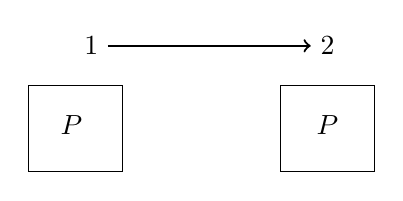
\begin{tikzpicture}
\node (atom1) at (0,1) {1};
\node (atom2) at (3,1) {2};
\node (atom3) at (-0.25,0) {$\enot P$};
\node (atom4) at (3,0) {$P$};
\draw[->, thick] (atom1) -- (atom2);
\draw (-0.8,-0.6) rectangle (0.4,0.5);
\draw (2.4,-0.6) rectangle (3.6,0.5);
\end{tikzpicture}
\end{center}
}

\item $\Box(P \eor Q)\vDash_\mlK  \Box P \eor \Box Q$
\myanswer{
\begin{center}
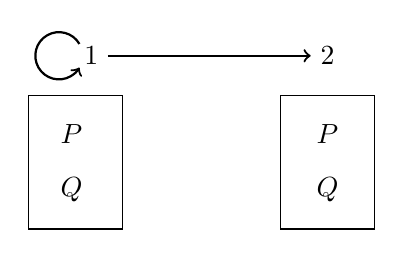
\begin{tikzpicture}
\node (atom1) at (0,1) {1};
\node (atom2) at (3,1) {2};
\node (atom3) at (-0.25,0) {$P$};
\node (atom4) at (3,0) {$\enot P$};
\node (atom5) at (-0.25,-0.7) {$\enot Q$};
\node (atom6) at (3,-0.7) {$Q$};
\draw[->, thick] (atom1)+(-0.15,0.15) arc (-330:-30:.3); 
%\draw[->, thick] (atom2)+(0.15,-0.15) arc (-150:150:.3); 
\draw[->, thick] (atom1) -- (atom2);
\draw (-0.8,-1.2) rectangle (0.4,0.5);
\draw (2.4,-1.2) rectangle (3.6,0.5);
\end{tikzpicture}
\end{center}
}

\item $\vDash_\mlK  \enot \Box (A\eand \enot A)$
\myanswer{
\begin{center}
\begin{tikzpicture}
\node (atom1) at (0,1) {1};
\node (atom3) at (-0,0) {$\enot A$};
\draw (-0.5,-0.6) rectangle (0.6,0.5);
\end{tikzpicture}
\end{center}
}

\item $\Box A\vDash_\mlK  A$
\myanswer{
\begin{center}
\begin{tikzpicture}
\node (atom1) at (0,1) {1};
\node (atom2) at (3,1) {2};
\node (atom3) at (-0.25,0) {$\enot A$};
\node (atom4) at (3,0) {$A$};
\draw[->, thick] (atom1) -- (atom2);
\draw (-0.8,-0.6) rectangle (0.4,0.5);
\draw (2.4,-0.6) rectangle (3.6,0.5);
\end{tikzpicture}
\end{center}
}
\end{earg}

\problempart
Present counter-interpretations to the following:
\begin{earg}
\item $\Box (M\eif O),\Diamond M\vDash_\mlT  O$
\myanswer{
\begin{center}
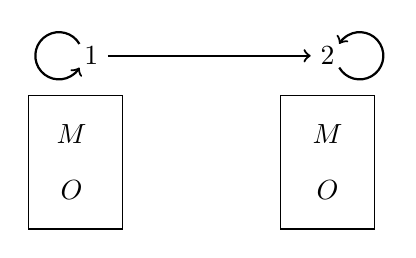
\begin{tikzpicture}
\node (atom1) at (0,1) {1};
\node (atom2) at (3,1) {2};
\node (atom3) at (-0.25,0) {$\enot M$};
\node (atom4) at (3,0) {$M$};
\node (atom5) at (-0.25,-0.7) {$\enot O$};
\node (atom6) at (3,-0.7) {$O$};
\draw[->, thick] (atom1)+(-0.15,0.15) arc (-330:-30:.3); 
%\draw[->, thick] (atom2)+(0.15,-0.15) arc (-150:150:.3); 
\draw[->, thick] (atom1) -- (atom2);
\draw[->, thick] (atom2)+(0.15,-0.15) arc (-150:150:.3); 
\draw (-0.8,-1.2) rectangle (0.4,0.5);
\draw (2.4,-1.2) rectangle (3.6,0.5);
\end{tikzpicture}
\end{center}
}

\item $\Box A\vDash_\mlT  \Box \Box A$
\myanswer{
\begin{center}
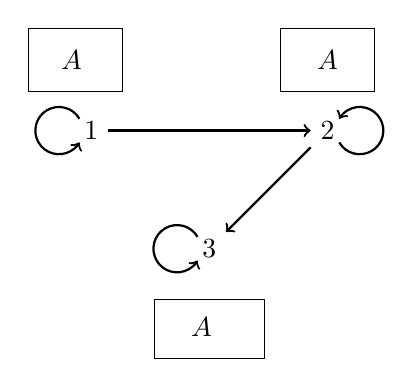
\begin{tikzpicture}
\node (atom1) at (0,1) {1};
\node (atom2) at (3,1) {2};
\node (atom3) at (1.5,-0.5) {3};
\node (atom4) at (-0.25,1.9) {$A$};
\node (atom5) at (3,1.9) {$A$};
\node (atom6) at (1.4,-1.5) {$\enot A$};
\draw[->, thick] (atom1)--(atom2);
\draw[->, thick] (atom1)+(-0.15,0.15) arc (-330:-30:.3); 
\draw[->, thick] (atom2)+(0.15,-0.15) arc (-150:150:.3); 
\draw[->, thick] (atom2)--(atom3);
\draw[->, thick] (atom3)+(-0.15,0.15) arc (-330:-30:.3); 
\draw (-0.8,1.5) rectangle (0.4,2.3);
\draw (2.4,1.5) rectangle (3.6,2.3);
\draw (0.8,-1.15) rectangle (2.2,-1.9);
\end{tikzpicture}
\end{center}
}
\end{earg}

\problempart
Present counter-interpretations to the following:
\begin{earg}
\item $\Diamond A\vDash_\mlSfour  \Box\Diamond A$
\myanswer{
\begin{center}
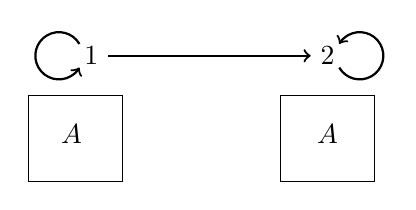
\begin{tikzpicture}
\node (atom1) at (0,1) {1};
\node (atom2) at (3,1) {2};
\node (atom3) at (-0.25,0) {$A$};
\node (atom4) at (3,0) {$\enot A$};
\draw[->, thick] (atom1)+(-0.15,0.15) arc (-330:-30:.3); 
\draw[->, thick] (atom2)+(0.15,-0.15) arc (-150:150:.3); 
\draw[->, thick] (atom1) -- (atom2);
\draw (-0.8,-0.6) rectangle (0.4,0.5);
\draw (2.4,-0.6) rectangle (3.6,0.5);
\end{tikzpicture}
\end{center}
}

\item $\Diamond A, \Box (\Diamond A \eif B)\vDash_\mlSfour \Box B$

\myanswer{
\begin{center}
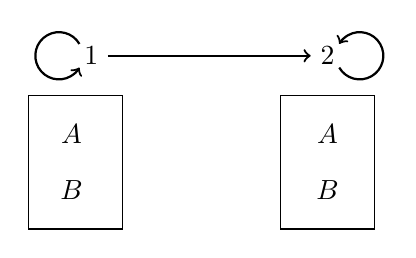
\begin{tikzpicture}
\node (atom1) at (0,1) {1};
\node (atom2) at (3,1) {2};
\node (atom3) at (-0.25,0) {$A$};
\node (atom4) at (3,0) {$\enot A$};
\node (atom5) at (-0.25,-0.7) {$B$};
\node (atom6) at (3,-0.7) {$\enot B$};
\draw[->, thick] (atom1)+(-0.15,0.15) arc (-330:-30:.3); 
\draw[->, thick] (atom2)+(0.15,-0.15) arc (-150:150:.3); 
\draw[->, thick] (atom1) -- (atom2);
\draw (-0.8,-1.2) rectangle (0.4,0.5);
\draw (2.4,-1.2) rectangle (3.6,0.5);
\end{tikzpicture}
\end{center}
}
\end{earg}


\chapter{Normal forms}\setcounter{ProbPart}{0}

\problempart
\label{pr.DNF}
Consider the following sentences:
	\begin{earg}
		\item $(A \eif \enot B)$
		\item $\enot (A \eiff B)$
		\item $(\enot A \eor \enot (A \eand B))$
		\item $(\enot (A \eif B ) \eand (A \eif C))$
		\item $(\enot (A \eor B) \eiff ((\enot C \eand \enot A) \eif \enot B))$
		\item $((\enot (A \eand \enot B) \eif C) \eand \enot (A \eand D))$
	\end{earg}
For each sentence, find an equivalent sentence in DNF and one in CNF.
\myanswer{We give a solution for (2). The truth table for $\enot (A \eiff B)$ is:
\begin{center}
\begin{tabular}{c c | l}
$A$ & $B$ & $\enot (A \eiff B)$\\
\hline
T & T & F \\
T & F & T \\
F & T & T \\
F & F & F \\
\end{tabular}
\end{center}
A sentence in DNF can be read off from lines 2 and 3:
\[(A \eand \enot B) \eor (\enot A \eand B)\]
and one in CNF from lines 1 and~4:
\[(\enot A \eor \enot B) \eand (A \eor B).\]}

\stepcounter{chapter} % Functional completeness

\chapter{Proving equivalences}\setcounter{ProbPart}{0}

\problempart
\label{pr.DNF2}
Consider the following sentences:
\begin{earg}
	\item $(A \eif \enot B)$
	\item $\enot (A \eiff B)$
	\item $(\enot A \eor \enot (A \eand B))$
	\item $(\enot (A \eif B ) \eand (A \eif C))$
	\item $(\enot (A \eor B) \eiff ((\enot C \eand \enot A) \eif \enot B))$
	\item $((\enot (A \eand \enot B) \eif C) \eand \enot (A \eand D))$
\end{earg}
For each sentence, find an equivalent sentence in DNF and one inCNF by giving a chain of equivalences. Use (Id), (Absorp), and (Simp) to simplify your sentences as much as possible.
\myanswer{We give a solution for (2). Removing `$\eiff$' and pushing negations inward is common to both:
\begin{align*}
	& \enot (A \eiff B)\\
	& \enot((A \eif B) \eand (B \eif A)) && \text{Bicond}\\
	& \enot((\enot A \eor B) \eand (B \eif A)) && \text{Cond}\\
	& \enot((\enot A \eor B) \eand (\enot B \eor A)) && \text{Cond}\\
	& \enot(\enot A \eor B) \eor \enot(\enot B \eor A) && \text{DeM}\\
	& (\enot\enot A \eand \enot B) \eor (\enot\enot B \eand \enot A) && \text{DeM}\\
	& (A \eand \enot B) \eor (\enot\enot B \eand \enot A) && \text{DN}\\
	& (A \eand \enot B) \eor (B \eand \enot A) && \text{DN}
\intertext{The result is now in DNF. To obtain a CNF, we keep going, using (Comm) and (Dist):}
& ((A \eand \enot B) \eor B) \eand ((A \eand \enot B) \eor \enot A) && \text{Dist}\\
& (B \eor (A \eand \enot B)) \eand ((A \eand \enot B) \eor \enot A) && \text{Comm}\\
& ((B \eor A) \eand (B \eor \enot B)) \eand ((A \eand \enot B) \eor \enot A) && \text{Dist}\\
& ((B \eor A) \eand (B \eor \enot B)) \eand (\enot A \eor (A \eand \enot B)) && \text{Comm}\\
& ((B \eor A) \eand (B \eor \enot B)) \eand ((\enot A \eor A) \eand (\enot A \eor \enot B)) && \text{Dist}\\
\intertext{The result can be simplified using (Simp):}
& (B \eor A) \eand ((\enot A \eor A) \eand (\enot A \eor \enot B)) && \text{Simp}\\
& (B \eor A) \eand (\enot A \eor \enot B) && \text{Simp}
\end{align*}}

\stepcounter{chapter} % Soundness


\end{document}
